%# -*- coding: utf-8-unix -*-
%%==================================================
%% thesis.tex
%%==================================================

% 双面打印


% \documentclass[doctor, fontset=nofonts, openright, twoside]{sjtuthesis}
\documentclass[bachelor, fontset=fandol, openany, oneside]{sjtuthesis}
% \documentclass[master, fontset=adobe, review]{sjtuthesis}
% \documentclass[%
%   bachelor|master|doctor,	% 必选项
%   fontset=adobe|windows,  	% 只测试了adobe
%   oneside|twoside,		% 单面打印,双面打印(奇偶页交换页边距,默认)
%   openany|openright, 		% 可以在奇数或者偶数页开新章|只在奇数页开新章(默认)
%   zihao=-4|5,, 		% 正文字号:小四、五号(默认)
%   review,	 		% 盲审论文,隐去作者姓名、学号、导师姓名、致谢、发表论文和参与的项目
%   submit			% 定稿提交的论文,插入签名扫描版的原创性声明、授权声明 
% ]

%%%%%roy7wt%%%%%
%
% 参考文献问题:
% 1)首先在每章前加入\bibliographystyle{sjtu2};
% 2)要用make clean thesis.pdf编译
%

% 逐个导入参考文献数据库
\addbibresource{bib/thesis.bib} %届时可以自行修改或者重新一个新的
%\addbibresource{bib/chap2.bib}

\begin{document}

%% 无编号内容:中英文论文封面、授权页
%# -*- coding: utf-8-unix -*-
\title{相似轨迹查询方法设计与实现}
\author{戚\quad{}文韬}
\advisor{朱燕民教授}
% \coadvisor{某某教授}
\defenddate{2017年5月15日}
\school{上海交通大学}
\institute{计算机科学与工程系}
\studentnumber{5130309593}
\major{计算机科学与技术专业}

\englishtitle{Design And Implementation of The Query Method of Searching Similar Trajectories}
\englishauthor{\textsc{Wentao Qi}}
\englishadvisor{Prof. \textsc{Yanmin Zhu}}
% \englishcoadvisor{Prof. \textsc{Uom Uom}}
\englishschool{Shanghai Jiao Tong University}
\englishinstitute{\textsc{Depart of Computer Science and Engineering, Shanghai Jiao Tong University} \\
  \textsc{Shanghai Jiao Tong University} \\
  \textsc{Shanghai, P.R.China}}
\englishmajor{Computer Science And Techonology}
\englishdate{May. 15th, 2015}


\maketitle
\makeenglishtitle

\makeatletter
\ifsjtu@submit\relax
	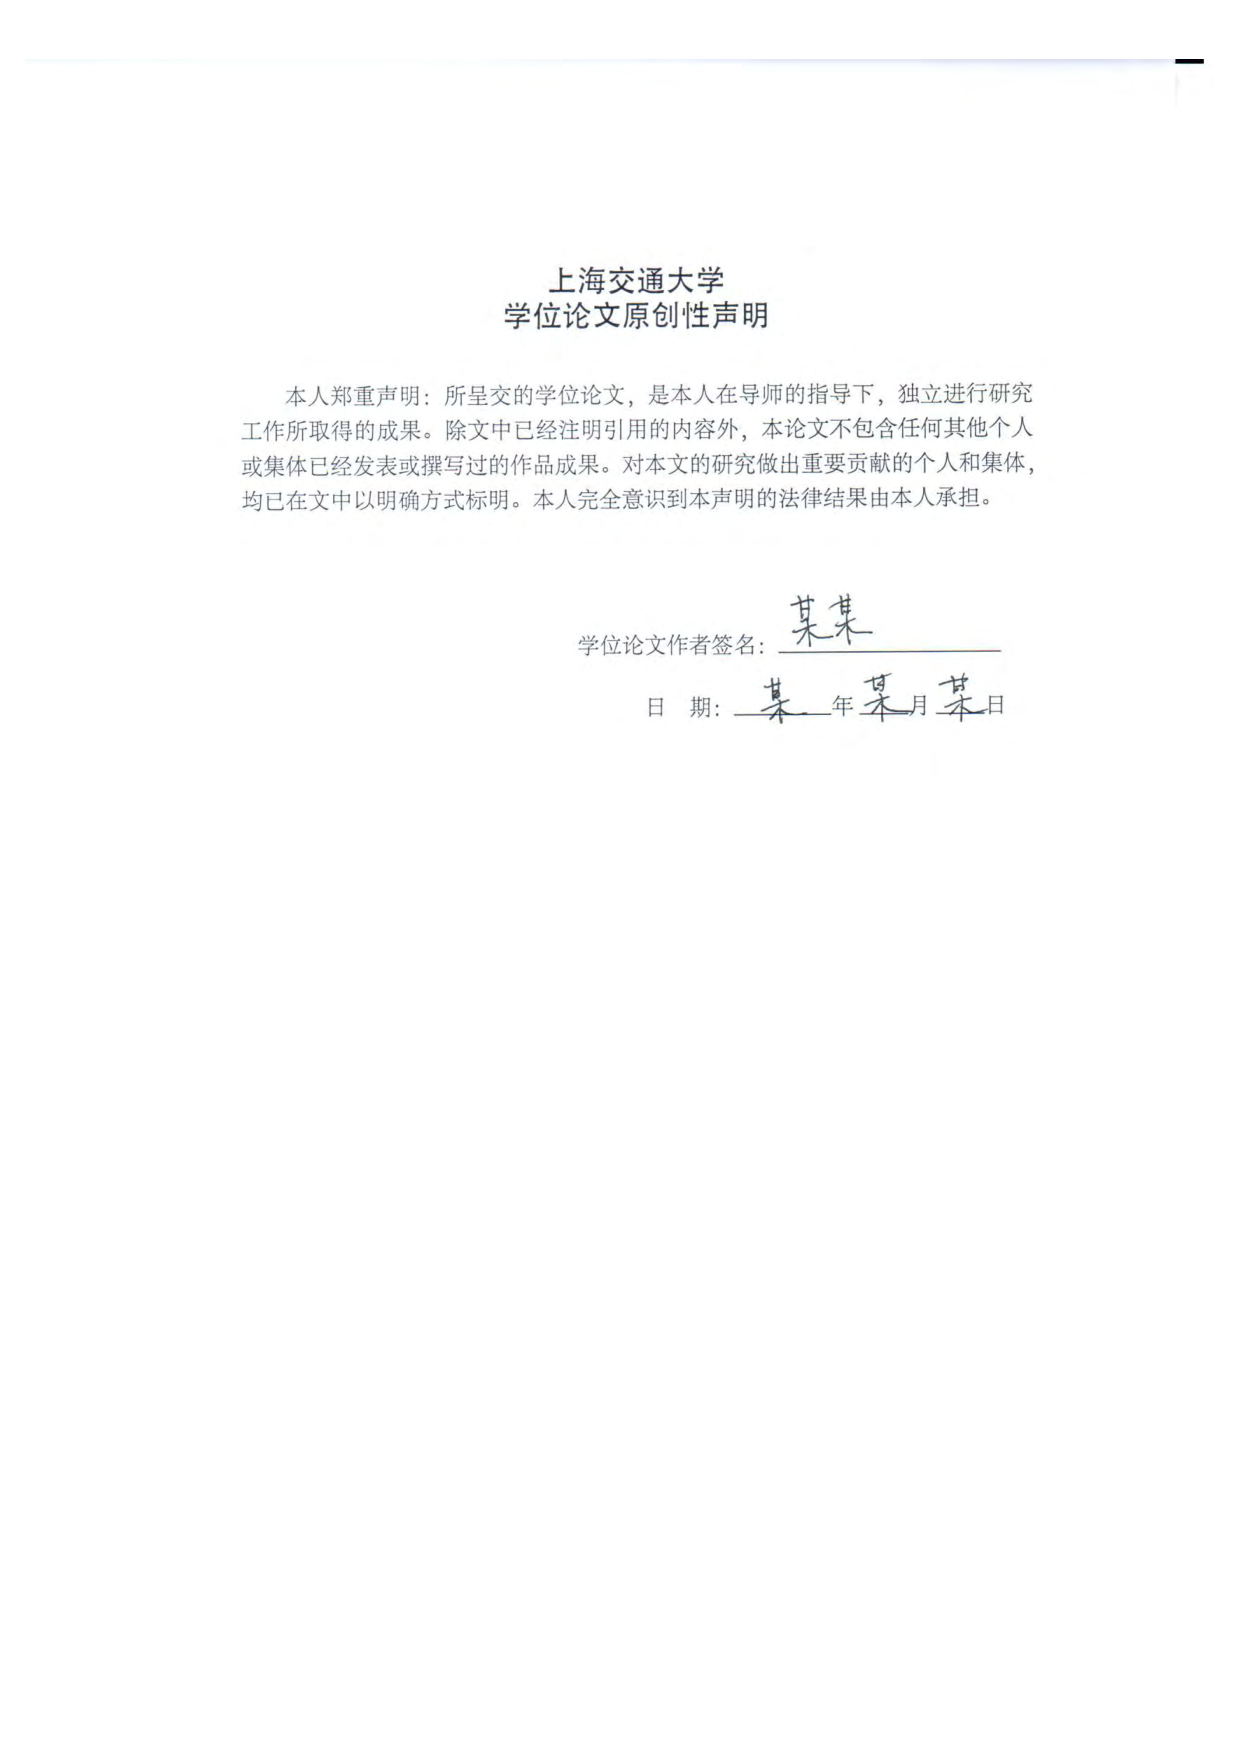
\includepdf{pdf/original.pdf}
	\cleardoublepage
	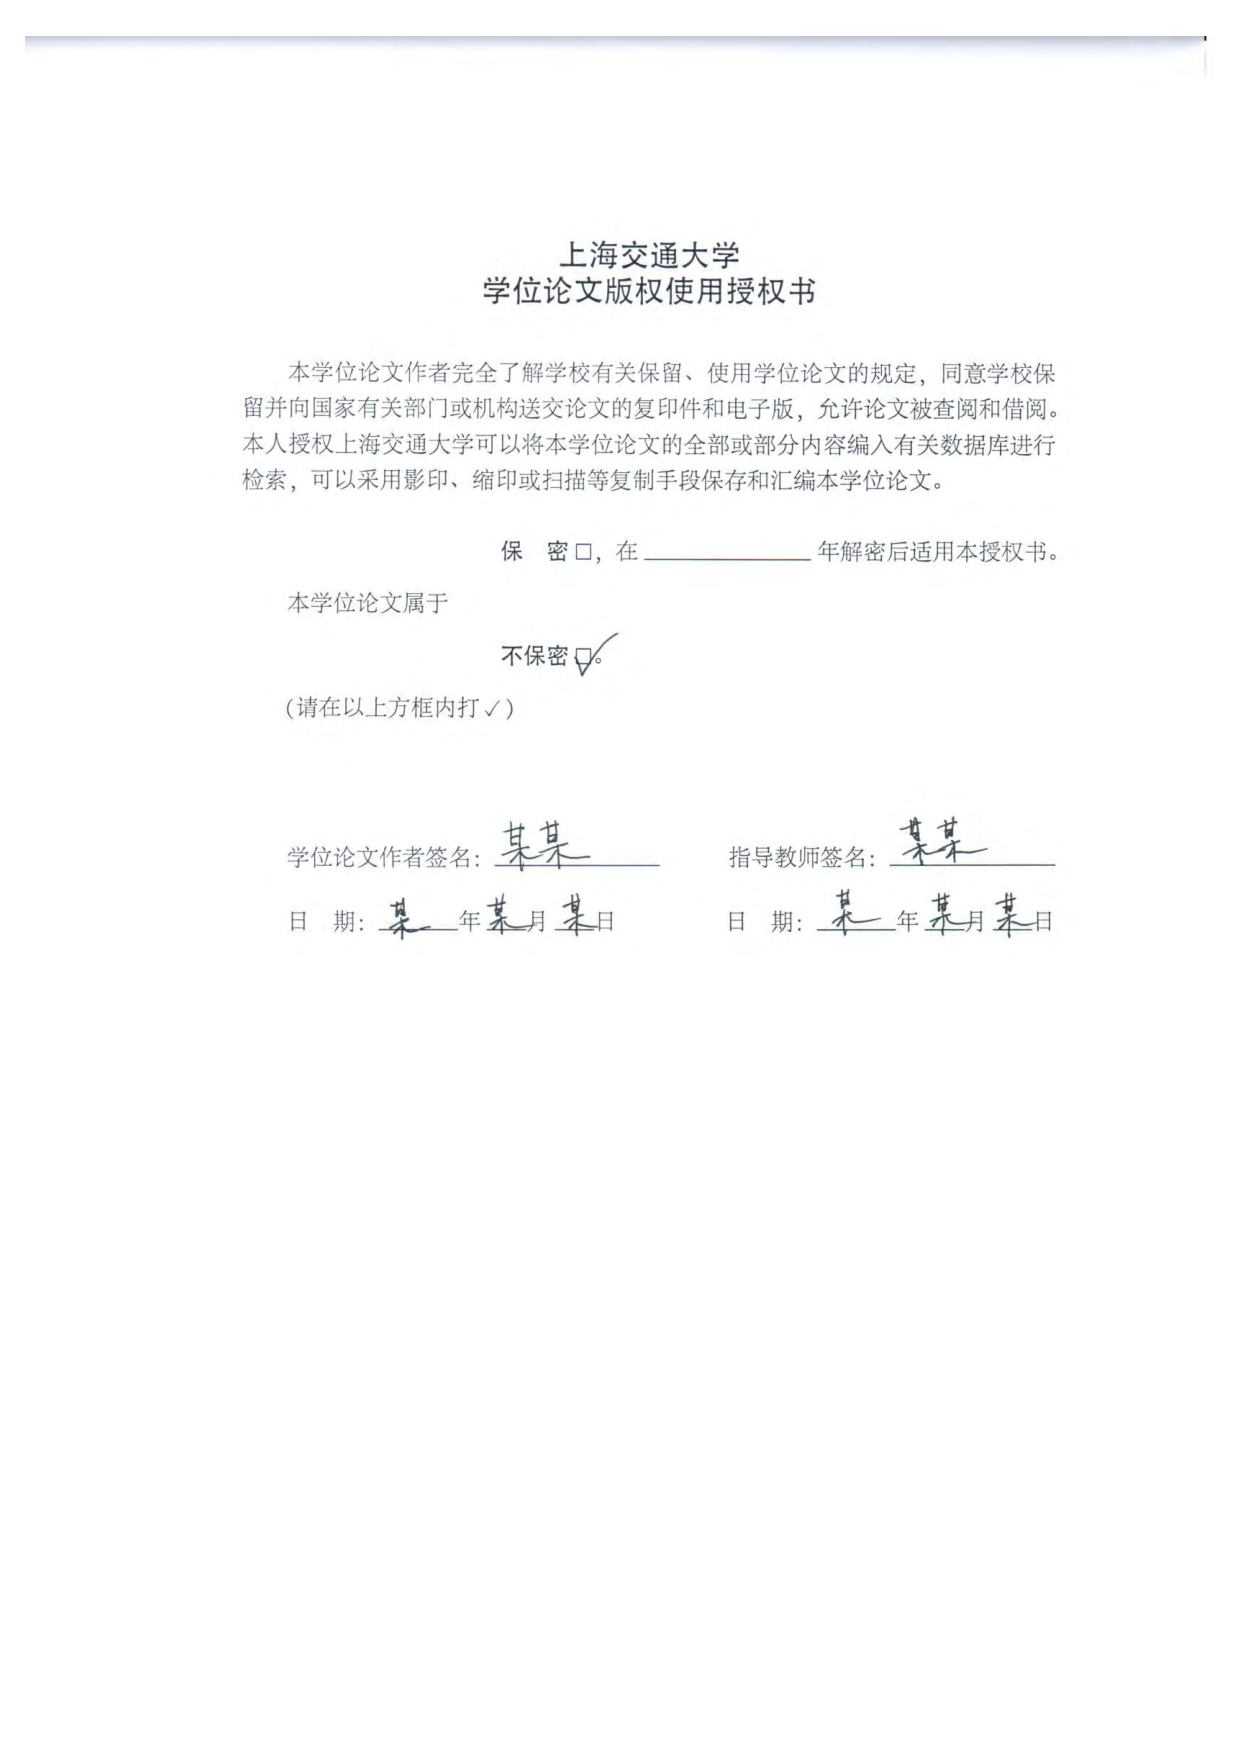
\includepdf{pdf/authorization.pdf}
	\cleardoublepage
\else
\ifsjtu@review\relax
% exclude the original claim and authorization
\else
	%\makeDeclareOriginal
	%\makeDeclareAuthorization
\fi
\fi
\makeatother


\frontmatter 	% 使用罗马数字对前言编号

%% 摘要
\pagestyle{main}
%# -*- coding: utf-8-unix -*-
%%==================================================
%% abstract.tex for SJTU Master Thesis
%%==================================================

\begin{abstract}
随着GPS技术和移动物体追踪技术的快速发展,相似轨迹搜索和轨迹匹配在许多应用中都有着很重要意义。在本文中,我们研究并实现一种基于地理位置点集的相似轨迹搜索。在这种搜索中,问题的输入通常为一组用户定义的有序或无序的轨迹点集,问题本质在于从轨迹数据集中找到k条最好连接这些查询点的已有轨迹,而从一般意义上说,这k条轨迹也可试做相对于查询点集的相似轨迹。不同之前传统的相似轨迹查询设计,我们对相似轨迹查询的实现重点更在于用户特定的轨迹点或轨迹中在地理语义上较为重要的轨迹点。不同于以一条轨迹作为数据所产生相似轨迹结果,我们的结果能满足用户特定的查询需求。

相似轨迹获取的前提在于对相似度方法的定义。在本文的应用场景中,我们首先将将一条轨迹相似度定义为相对于查询点集的连接程度。对于用户实际运用而言,查询点集数量一般较少。本文根据这一点实现多方面的基于\emph{增长型k最近邻}查询的相似轨迹查询方法。在空间相似度程度上,我们定义上界与下界以用于剪枝和优化查询到的相似轨迹。将k最近邻查询通过最好优先搜索或深度优先搜索的扩展,实现一个轨迹点在R树数据结构上的查询,以满足增长型k最近邻查询的需求,且保证了搜索的高效性和内存存储空间的保证。之后再对搜索参数进一步动态调整以加速相似轨迹搜索的过程。本文认为这种基于地理位置点的相似轨迹查询在为在路径规划、轨迹推荐、交通流量分析、拼车出行和基于地理位置的一些应用中这种基于查询点的相似轨迹查询都能够在通常意义上发挥作用。
\\
\\
\keywords{\large 相似轨迹查询 \quad k最近邻 \quad 算法设计 \quad 优化}
\end{abstract}

\begin{englishabstract}
With the quick development of Global Position System technology and moving-object tracking technology, similar trajectory search and matching is becoming increasingly important in many applications. In this work, we study and implement a new type of similar trajectory searching based on geographical locations, where the input of search is a small set of user-defined location points with or without order restraint. The essence of searching problem lies in finding the k Best Connected Trajectories in the trajectory database to connect these locations points. To some extent, we consider these trajectories as the result of similar trajectory searching. Different the traditional search of similar trajectory, we focus more on the location points that users specifically define or the ones weigh more in the geographical context. This type of search can satisfy the user-defined demand more than the gerenal-purpose similar trajectory search before.

In our work, the prerequisite of searching similar trajectory is to define the similarity function. We first define the function to measure how well a trajectory connects the query location points in our application context. In practice, the number of query points tends to be relatively small. Upon this observation, we implement the search of similar trajectory based on the \emph{Incremental k-NearestNeighbor} algorithm we proposed. The Incremental k-NearestNeighbor prunes and refines the search process by the pre-defined upper bound and lower bound of trajectory similarity. In this algorithm, we extends the k-NearestNeighbor by best-first search of depth-first search on a spatial index structure, R-tree, in order to guarantee the efficiency of searching and lower the lost of memory usage. Another contribution of our work lies in the further optimization of the search process by dynamically adjusting the searching parameters. We believe that this type of search may bring significant benefits to users in many applications, such as route planning, trajectory recommendation, traffic analysis, carpooling and location-based services in general.

\englishkeywords{\large Similar trajectory search,k-NearestNeighbor, Algorithm design, Optimization}
\end{englishabstract}



%% 目录、插图目录、表格目录
\tableofcontents
\listoffigures
\addcontentsline{toc}{chapter}{\listfigurename} %将插图目录加入全文目录
\listoftables
\addcontentsline{toc}{chapter}{\listtablename}  %将表格目录加入全文目录
\listofalgorithms
\addcontentsline{toc}{chapter}{算法索引}        %将算法目录加入全文目录
%\include{tex/symbol} % 主要符号、缩略词对照表

\mainmatter	% 使用阿拉伯数字对正文编号

%% 正文内容
\pagestyle{main}
%# -*- coding: utf-8-unix -*-
%%==================================================
%% chapter01.tex for SJTU Master Thesis
%%==================================================

%\bibliographystyle{sjtu2}%[此处用于每章都生产参考文献]

\chapter{绪论}
\label{chap:introduction}

\section{轨迹数据处理现有工作的概述及评价}
\label{sec:background}

计算机信息处理和存储技术的高速发展和快速普及,使得各个应用行业和科研领域的工作规模在数据上呈现爆炸式的增长。早期人们从数据规模出发用大数据(\emph{Big Data})对这一概念进行定义,现在大数据这一定义更多地从信息处理技术和需求方法出来,代表着我们从大数据分析与应用中所需求的新的应用和新的发展。随着计算机飞速进步的处理能力,我们能够从大数据挖掘中获取到我们所需要的应用价值。

传统企业数据、机器与传感器数据和社交数据被认为是如今大数据大致的三个类别。轨迹大数据主要属于机器与传感器数据。现代社会地理位置获取和移动计算科技进步,促使轨迹数据的大规模发展。这些轨迹数据体现了例如人类,车辆以及动物等移动物体的移动多样性。在过去十几年间,许多旨在处理、管理和挖掘轨迹数据的算法与技术许多应用中有着广泛而重要的应用价值。如今以轨迹数据挖掘为首的轨迹数据处理技术已经日趋系统且规范,从轨迹数据生成,到轨迹数据预处理,再到轨迹数据管理,最后到多样的数据挖掘任务(例如轨迹模式挖掘、轨迹异常检测、轨迹分类等等)。已有轨迹处理和轨迹挖掘的技术在相互应用中有着重要的联系与关联,轨迹数据转化成其他轨迹形式,例如图、矩阵和张量的方法也在越来越多的轨迹数据挖掘和机器学习领域有着常见的应用。

轨迹从概念上定义是一个移动物体的移动轨迹,轨迹数据可以用于许多领域的复杂分析。例如,公共交通系统可以应用过去时刻的轨迹数据分析交通流量模式并找出致使交通拥塞的原因;生物领域的动物长途迁移轨迹或是短途移动变化可以为人类提供宝贵的数据分析人类活动对生态环境的影响程度;还可以通过分析数据预测城乡车辆移动情况并及时提供符合公众出行的公共交通支持。其他应用领域也包括了路径优化设计,公共交通安全管理和基于兴趣点的用户个性化服务。

基于以上应用情景,轨迹数据挖掘在计算机科学、社会学和地理学领域都变得愈发重要。在轨技数据挖掘领域研究从深度和广度都已经取得了不错的成果,从图\ref{fig:1-1}\cite{zheng2015trajectory}可以看出当前轨迹数据挖掘与处理的基本研究步骤。本课题相似轨迹查询方法设计与实现主要基于其该范例中的轨迹预处理与轨迹数据索引与获取这两个领域中已存在的方法,并结合自己的理解和数据的格式实现改善和创新。

\begin{figure}[!htp]
  \centering
  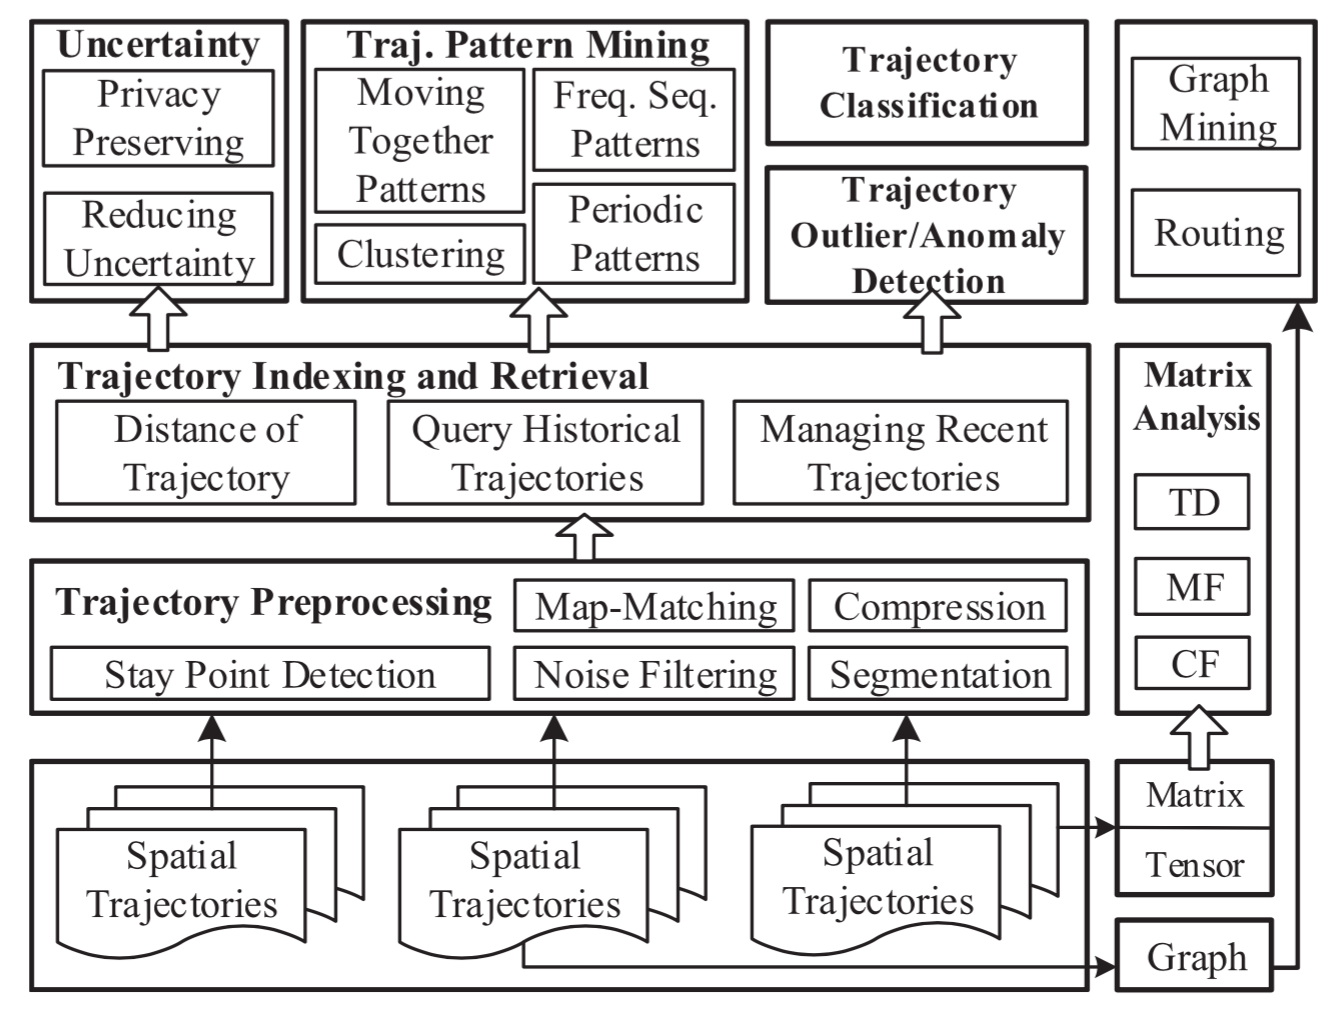
\includegraphics[width=0.9\textwidth]{chapter01/paradigm.png}
  \bicaption[fig:1-1]{轨技数据挖掘范例}{轨技数据挖掘范例}{Fig}{Paradigm of trajectory data mining}
\end{figure}

大量空间轨迹数据为我们提供了分析移动物体移动方式的可能性,这种移动方式的分析可以体现出单个轨迹所包含的某种特定移动方式或是一组轨迹所共享的相似移动方式。通常情况下相似轨迹查询是基于时空关系的查询,除此之外有些情况下一些相似轨迹查询会增加特定的查询条件,例如最快速度、偏移方向或是在规定的时间段内经过特定地理区域等等条件。在相似轨迹查询中缺少时间维度参数(时间戳或是时间段)是可以接受的,加入时间参数的相似轨迹查询本文将他们视为其中的一种特殊情况处理。
\\

\subsection{轨迹查询概念简介}
\label{sec:requirements}
完成在轨迹数据库中复杂的轨迹查询操作是复杂且费时的操作,因为轨迹数据库的规模一般是非常庞大的。因此,轨迹数据库的一个重要点事支持高效的轨迹索引以加速轨迹插叙过程。通常情况下,时空数据的索引技术是空间数据索引辅以时间度量参数。轨迹查询\cite{zheng2011computing}既关注经过的地理位置的拓扑位置顺序,也关注空间物体之间的距离度量,从简单的欧式距离度量到复杂的轨迹之间相似性。从大体上说,如今的轨迹查询依照时空关系分为三类:1)$P$-$query$,查询满足特定轨迹段或者时空关系的兴趣点或者查询针对某些兴趣点满足时空关系的轨迹;2)$R$-$query$,根据给定的时空区域查询轨迹或者给定轨迹查询目的区域,3)$T$-$query$, 查询在一组轨迹数据集中查询相似轨迹或在给定的距离阈值内查询轨迹。
\\

\subsection{相似轨迹查询应用现状}
\label{sec:requirements}
相似轨迹查询主要是基于上述的轨迹查询方法中$P$-$query$和$T$-$query$展开的。

$P$-$query$主要应用在给定地理位置点后找到满足时空关系的轨迹或者轨迹段。单点轨迹查询找到针对某一给定地理位置点的最近轨迹。多点轨迹查询在给定一组地理位置点集后在轨迹数据里中找到能在地理位置意义上连接查询点集的多条轨迹。前者用以找到某一地理位置范围内的潜在轨迹。后者在制定行进轨迹路线中有着很好的应用。$T$-$query$通常通过聚类或分类轨迹在轨迹数据库中查询轨迹。轨迹分类和聚类算法在许多应用中有着广泛的应用,例如基于移动物体特征的轨迹测或是分析路网流量结构,在轨迹集合发现共同的子轨迹以及查询与目标轨迹在欧式距离上最接近的轨迹集合。

基于$P$-$query$的查询主要是衡量点到轨迹的中最近点的距离。目前也常通过拓展这一思路当多点的$P$-$query$查询以评价一条轨迹连接多个查询点的好坏。在$T$-$query$这一查询类型方面则有很多较为成熟的方法主要的不同在于他们各自的相似距离函数的定义,例如动态时间规划轨迹方法(Dynamic Time Warping)[ref]、最长公共子序列方法(Longest Common Subsequence)[ref]、基于编辑代价的方法(Edit Distance With Real Penalty)[ref]和基于序列编辑距离的方法(Edit Distance on Real Sequences)等等。这些方法在初期主要应用于时序相关的数据上,但是由于轨迹在某种意义上可以看成是多维度上的时序数据,上述的相似距离方法则可以应用上轨迹数据上。
\\

\section{相似轨迹查询问题描述}
\label{sec:requirements}

\subsection{问题大致描述}
\label{subsec:question}
随着轨迹数据大规模的发展与存储,在日常生活中,如何高效查询轨迹对于用户或是在工业领域都有着重要的意义。特定情况下,查询类型也会根据需求有着变化。相似轨迹查询属于轨迹查询中的一种。在这里我们队相似轨迹查询问题进行大致描述;给定一组表示一条轨迹的轨迹数据点$Q$和轨迹数据库$D$,查询出在地理形状上与这些轨迹点所描述的轨迹的k条最相近的轨迹。

\subsection{相似轨迹查询方法设计概述}
\label{subsec:requirements}
本文研究的相似轨迹查询方法主要基于位置定的查询,即查询主要是基于一组有序或是无序的地理位置点。查询的首相要目标是从轨迹数据库中找出连接查询位置点的k条最佳连接轨迹(K Best-Connected Trajectories)使得这k条轨迹能够在地理位置上连接给定的未指定。不同于传统形状或其他查询标准通过给定一条轨迹的相似轨迹查询,本文的相似轨迹查询主要针对于所查找到的轨迹对于给定的一组轨迹点连接性的优劣。

如图\ref{fig:1-2}所示,通过点击地图或图像地理解码给定一组地理位置点(图中点注释),我们可以从数据库中获取找一条能够连接给点地理位置点原始轨迹(图中线注释),该实例体现出本相似轨迹查询方法在能够在包括旅游路线规划等新兴应用中更好地服务用户。与此同时,这种相似轨迹查询能还能在以上场景有所应用:旅行社或自由行游客对出行经典的路径规划;动物园能调查出动物对到某些特定地点的最短路径;交通运输部门对本地市民城乡情况的规划。

\begin{figure}[!htp]
  \centering
  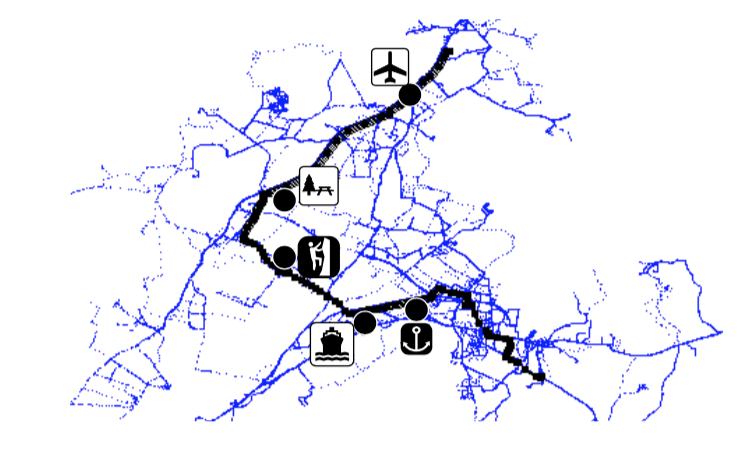
\includegraphics[width=0.5\textwidth]{chapter01/search-example.png}
  \bicaption[fig:1-2]{基于位置点的相似轨迹查询}{基于位置点的相似轨迹查询}{Fig}{Similar trajectory search by locations}
\end{figure}

大体上,k条最佳连接轨迹查询基于的地理位置点需要具备必要的经纬度信息$(latitude,longitude)$。这些经纬度位置地点可以是旅游景点,不明确的沙滩或是任何一处地理坐标。用户可以通过决定轨迹连接有序或是无序以决定查询结果。例如一个简单的查询包括三个地理位置点 $A$,$B$,$C$

\begin{displaymath}
	{A_{(37.2601, 122.0941)}, B_{(37.2721, 122.0648)}, C_{(37.3344,122.1538)}}
\end{displaymath}

其中(37.2601, 122.0941)代表A点的经纬度地理坐标。如果查询附带有序条件,则查询轨迹结果应保留轨迹点之间的相对顺序性,即$A \rightarrow B \rightarrow C$。传统的相似轨迹查询方法显然无法解决查询结果与查询条件之间有序一致性。另外,本文所提出的轨迹查询方法基于任意的地理位置点使得查询模式更加多样和灵活。从本质上而言,这种这种查询方法的设计基于传统的单点查询方法以寻找针对某一位置的最为临近轨迹。

为了实现这一相似轨迹查询方法,本文首先对一组给定地理位置点中的每一个点进行基于点的查询以从数据库中找到最近的轨迹点。如果查询结果存在,通过对每一个结果的汇总所得出的轨迹从理论上而言是最接近查询点的一条轨迹且对给定的地理位置点具有良好的连接性。从这个思路出发,本文拓展K最近邻(k-NearestNeighbor algorithm)算法并提出增长性K最近邻($Incremental$ $k$-$NN$ $algorithm$)算法。该算法增长性获取每个查询位置点的最近轨迹并不断检查以查询到的轨迹。通过自定义的轨迹相似性上界与下界,借鉴备选和筛选的算法设计思路(candidate-refinement)来进行优化与剪枝。利用R树(R-Tree)作为地理位置点的索引结构,算法实现过程中根据具体计算机情况和性能需求选择性使用最好优先搜索(best-first)方法或是深度优先搜索(depth-first)方法进行查询。
\\

\section{相似轨迹查询应用价值}
\label{sec:application value}
相似轨迹查询系统在实际情景中具有广泛的应用价值。在路径规划应用方面上,相似轨迹查询从已记录的历史轨迹中,根据用户定义有序或无序的旅游景点顺序,给出k条大致符合出行路径的历史轨迹基于用户参考并选出用户自己偏好的出行路径;在轨迹推荐或拼车推荐方面上,由于限号或出行限制问题,可以通过在历史轨迹中查询相似的轨迹查询出是否有在上下班或平时出行模式较为相似的多名用户,选择在有出行限制的时段与别的用户共享出行设备;在交通分析方面,相似轨迹查询可以为公安行业根据几个具体的地理位置点锁定一辆具有车载GPS设备的车辆。除此之外,相似轨迹查询的具体应用还有许多,不予以赘述。

\section{困难和挑战}
\label{sec:difficulty}
相似轨迹查询方法的设计与实现存在的以下主要的困难和挑战:1)高效准确实现相似轨迹查询。由于轨迹数据集的规模较大,通过常规查询和搜索会耗用大量时间和空间,而且在搜索过程中还要避免一些错误数据的加入。2)基于分布式的相似轨迹查询。相似轨迹查询领域的已有工作较为丰富,但是在单机层面上的查询处理。对于轨迹大数据处理而言,将相似轨迹查询移植与分布式环境操作是必要过程。3)实现基于相似轨迹查询功能的软件系统。轨迹数据处理的价值在于通过轨迹数据处理为每个客户提供特定服务。在相似轨迹查询中,需要提供一个用户界面为用户查询相似轨迹并将轨迹可视化的软件系统,在满足高效查询过程中需要保证良好的软件系统交互性。

\section{论文结构}
\label{sec:requirements}
\textbf{重写}
%本毕业论文主要结构为:本章介绍轨迹查询大致概念与相似轨迹查询现状与方法大体设计;第二章介绍实现相似轨迹查询方法设计的相关工作;在第三章详细讨论算法实现细节与优化问题处理;第四章中讨论相似轨迹查询和分布式结合具体过程与算法实现;实验过程和结果会在第五章中予以描述并在第六章为本文做结论。
\\

\section{本章小结}
\label{sec:requirements}
本章节已经初步介绍了相似轨迹查询这一概念和其相关背景,由于目前的在轨迹数据处理已经系统和规范的处理流程,轨迹数据挖掘这一领域的方法技术也已经较为成熟且丰富,通过学习传统的相似轨迹查询方法和他们各自的应用经验,本文所提出的方法在已有成果的基础上进行进一步的创新与优化,便可以使得相似轨迹查询方法与传统的相似轨迹查询有着较大的不同,且具有特定查询环境上的查询优势与性能优化。在对相似轨迹查询问题进行大致描述后,本文对解决这一问题在现实生活中有哪些具体的应用进行展开,并初步描述解决相似轨迹查询这一问题所产生的实际价值。

解决相似轨迹查询这一问题的过程中也伴随着一些具体的困难与挑战。本文通过拓展如今最为基本的k最近邻数据挖掘技术,以实现基础的相似轨迹查询方法为基本理论目的,移植单机运行代码至分布式环境系统为应用目标,开展毕业设计课题。



%# -*- coding: utf-8-unix -*-
%%==================================================
%% chapter02.tex for SJTU Master Thesis
%% related work
%%==================================================
%\bibliographystyle{sjtu2}%[此处用于每章都生产参考文献]

\chapter{ 相关工作 }
\label{chap:related}

\section{相似度方程定义}
\label{sec:similarityfunc}
相似轨迹查询工作在某种意思上和时序数据相似查询共享一些方法定义。相似轨迹查询的首要步骤通过某种选定轨迹与轨迹点间的距离度量来定义相似度(或称为距离)方程,之后是设计高效的查询过程算法来解决从大规模数据库中找到符合要求的备选轨迹。定义相似度方法在过去有许多深度的讨论,之前的工作有通过利用离散傅里叶变化(Discrete Fourier Transform)[Ref bylocation2]将轨迹数据转化为多维空间上的点,任何通过比较这些点在特征空间上的欧式距离来比较轨迹数据时间的相似性。之后有科研人员在此工作成果的基础上通过改善实现子轨迹的匹配查询,并验证了离散小波变换(Discrete Wavelet Transform)的可行性。切比雪夫多项式(Chebyshev polynomials)在轨迹近似和索引方面有被证明是可应用的。但是这些方法的前提调前是需要轨迹上时序上具有相同的长度,因此这些转变返程所提供的相似度方法不适用与本文所提出的相似轨迹查询。
\\

\begin{figure}[!htp]
  \centering
  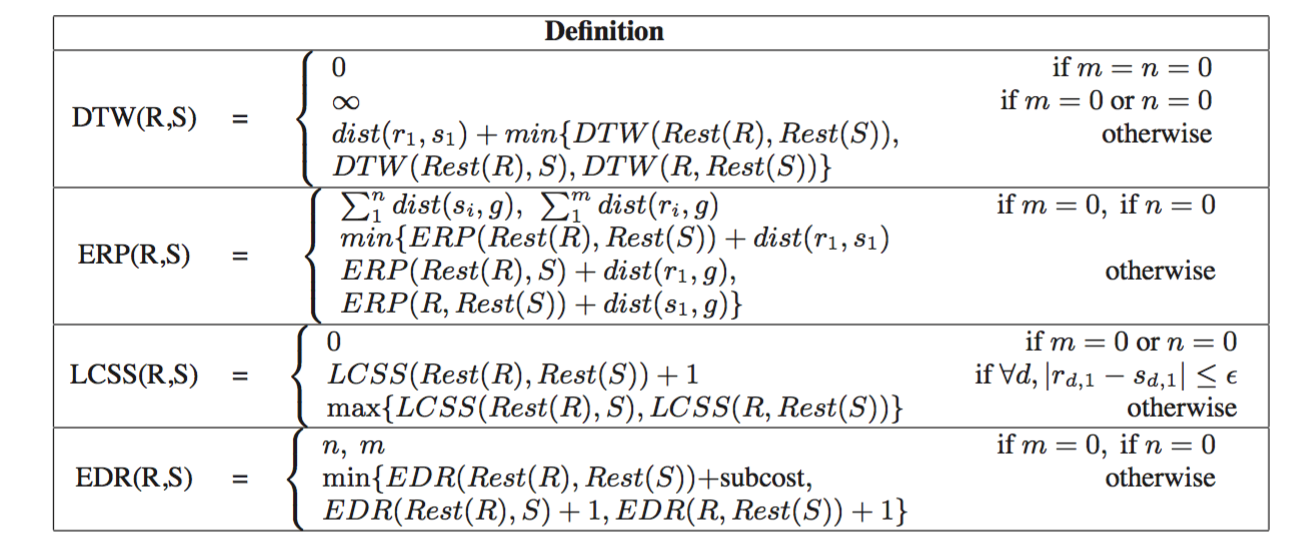
\includegraphics[width=1.0\textwidth]{chapter02/definition.png}
  \bicaption[fig:2-1]{这里将出现在插图索引中}{相似度函数定义\footnotemark[1]}{Fig}{Definition of distance functions}
\end{figure}
\footnotetext[1]{$dist(ri,si)=$ L1 or L2 norm; $subcost = 0$ if $r1,t−s1,t$, else $subcost= 1$}

图\ref{fig:2-1}是典型且常用的相似度方程定义。这些方程根据自身特点与优势应用于不同的场景中,包括欧氏距离方程(Euclidean Distance),动态时间规整(Dynamic Time Warping),最长公共子序列算法(Longest Common Subsequence),基于编辑代价的方法(Edit Distance With Real Penalty)和基于序列编辑的距离方法 (Edit Distance on Real Sequences)。动态时间规整(DTW)方法在比较轨迹之间相似性的过程中采用了时间偏移(time-shifting)来使得轨迹中的一些点可以尽可能多地重复出现以实现最好效果的校准。但这种方法在原有轨迹数据点出现误差(或称为噪声点)的时候会影响比较的准确性因为所有的点都需要被匹配。相比如动态时间规整方法(DTW),最长公共子序列(LCSS)选择忽略某些点以避免对他们的重排序过程,从结果上而言这种方法舍弃了偏离采样的误差点以提高了准确性,但需要人为预定距离阈值以判断什么数据属于误差点。基于编辑代价的距离方法(EDR)与LCSS方法类似,他们最初提出是为了解决字符串匹配问题,在轨迹数据匹配这一方面他们均采用一个阈值参数来判断两个点是否匹配,但EDR考虑了距离之间的衡量代价以决定是否将两个点进行匹配。在此基础上基于序列编辑的距离方法(ERP)结合EDR和DTW方法选择固定点进行距离计算。

相似度方法通常根据具体的应用进行具体的选取。但上述的相似度方法主要是基于轨迹与轨迹之前相似度的查询,在本文设计的相似轨迹查询方法上的应用度并不理想,本工作的查询条件是基于一组地理坐标点的查询,并且工作更关注与一条轨迹是否能够很好地连接上给定的一组查询点,从而提供基于轨迹点的相似轨迹结果。因此,在这样的情景下,我们需要定义一个新的相似度方程。
\\

\section{轨迹数据预处理}
\label{sec:preprocess}

\subsection{WGS84坐标系统转换至GCJ-02坐标系统}
\label{subsec:coord-transform}
WGS84(World Geodetic System1984)坐标系统是GPS数据所基于的坐标系统,这一坐标系是通过世界卫星观测站所检测到的地理坐标。这一坐标系并不能直接应用在中国国家的地图坐标显示中,因为中国国家会测局在地理信息系统中使用的是基于GCJ-02的坐标系统,这一坐标系统也称为火星坐标系统。如果直接将WGS84坐标数据应用于使用GCJ-02的地图显示接口,则会造成100米到700米范围内的显示误差。同理,用户使用GCJ-02地图点击获得的地理位置查询点也会在相似轨迹查询中因为与WGS84坐标系统的偏差因素造成查询结果的不准确性。在轨迹预处理最开始先将WGS84坐标数据根据已有的算法\footnotemark[1]参考转换成GCJ-02系统下的坐标
\footnotetext[1]{https://github.com/googollee/eviltransform}
\\


\subsection{轨迹数据简化}
\label{subsec:trajectory simplification}
轨迹数据预处理中,轨迹数据的简化(或压缩)是比较重要一步。轨迹数据简化主要是指在保证轨迹的可利用性与大致准确的同时减少轨迹的点数目,以达到轨迹数据的传输、处理和存储上减少开销的目的。在本文的应用场景中,我们首先采用\emph{Douglas}–\emph{Peucker}算法来完成我们的轨迹简化任务。该算法的主要思路在于将通过分而治之,将曲线轨迹表示成一系列点的方法,从而减少点的数目。如今GPS的数据采样通常较为频繁,因此在我们对轨迹处理的范围上来所,我们可以近似地将我们所运用的数据集中的轨迹看成是一条连续的曲线,通过\emph{Douglas}–\emph{Peucker}算法以及我们人为设定简化阈值,我们可以高效且合理地进行轨迹简化。

\begin{algorithm}
% \begin{algorithm}[H] % 强制定位
\caption{Douglas-Peucker算法}
\label{algo:dp-ts}
\begin{algorithmic}[1] %每行显示行号
\Require 一条原始轨迹数据$Traj$, 简化阈值$\epsilon$ % 输入
\Ensure 简化后的轨迹$Traj'$ % 输出
\State $dis\_max \gets 0$;$index \gets 0$
\For{$i = 1$ to $Traj.length-1$}
	\State $temp\_dis \gets$ Traj[i]'s perpendicular Distance to Line(Traj[0], Traj[Traj.length])
	\If{$temp\_dis > dis\_max$}
		\State $dis\_max \gets temp\_dis$;$index \gets i$
	\EndIf
\EndFor
\If{$dis\_max > \epsilon$}
	\State half\_left $\gets Douglas$-$Peucker(Traj[0:index],\epsilon)$;
	\State half\_right $\gets Douglas$-$Peucker(Traj[index:Traj.length],\epsilon)$;
	\State $res \gets$ half\_left $\bigcup$ half\_right;
	\Else
	\State $res \gets \{Traj[0], Traj[Traj.length]\}$;
\EndIf	
\State \textbf{return} $res$;
\end{algorithmic}
\end{algorithm}

算法\ref{algo:dp-ts}在首先连接轨迹首尾两点$Traj[0],Traj[Traj.length]$,遍历轨迹一遍得到离线段距离最大的点$Traj[index]$,计算该距离并与预先设定的阈值$\epsilon$比较。如果大于阈值$\epsilon$,则将轨迹以$Traj[index]$为中点分为两端,迭代重复上述工作;如果小于阈值$\epsilon$,则直接将线段段作为曲线的近似以做简化。当曲线完成上述任务,依次连接处理好的子线段,完成轨迹简化任务。
\\

\section{轨迹数据索引与获取}
\label{sec:index}
空间数据结构对从一个大规模轨迹数据集中获取特定轨迹数据是十分重要的。效率问题是查询大规模数据库或数据集来获取信息的首要考虑因素。而查询效率十分依赖于合理的轨迹索引。轨迹数据根据数据特点的不同姓对索引技术也有着特殊的要求。目前主流的索引技术主要有三类:1)基于空间维度的索引,利用R树(R-tree)索引进行查询。通过3DR树(3D R-tree)或者STR树(STR-tree)进行带有时间维度的查询;2)利用多版本的数据结构,根据特定情况使用 MR树(MR-tree)、HR树(HR-tree)、MV3R树(MV3R-tree)等等;3)将空间划分网格结构然后对应每个网格建立对应的空间索引,这类数据结构包括MTSB树(MTSB-tree)和SETI。本文中我们使用R树这一最基本的数据结构,其满足我们对算法的实现需求。

R树数据结构在空间数据库中应用广泛,许多轨迹索引结构大体上是基于R树进行拓展。R树结构是一个平衡树结构,R树中的每一个节点代表包含其所有子节点一个区域,这个区域通常被称为最小区域箱(Minimum Bounding Box)。节点中的每一个数据体指向对应的子节点的最小区域箱信息。R树搜索的关键字是最小区域箱中的每一个节点。如图\ref{fig:2-2}所示的是R树数据结构的2种表现形式。在\ref{fig:2-2}(b)中我们看到树结构而图\ref{fig:2-2}(a)描述了数据和最小边界箱是如何分布在空间中的。
\\

\begin{figure}[!htp]
  \centering
  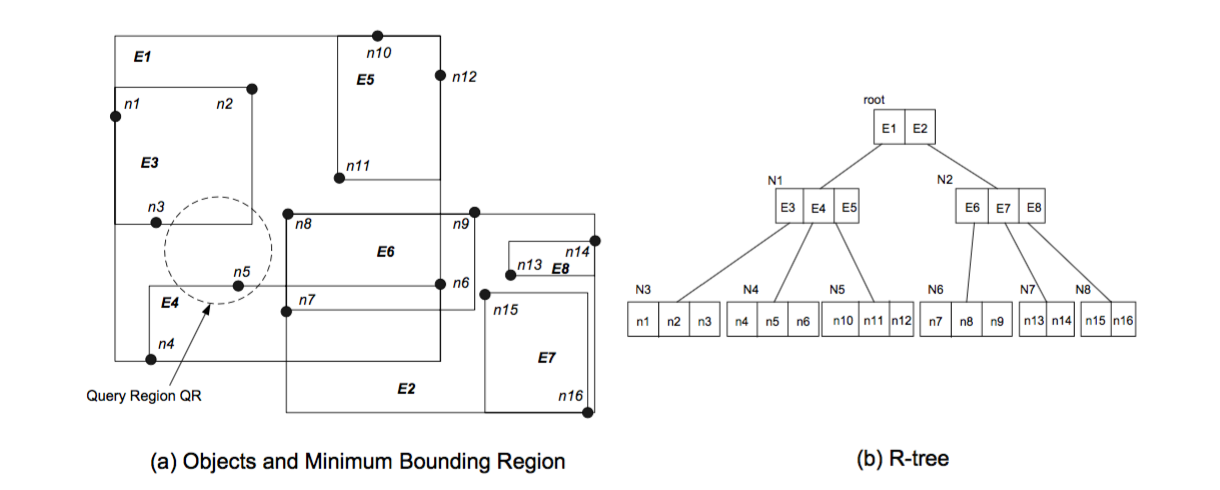
\includegraphics[width=1.0\textwidth]{chapter02/rtree.png}
  \bicaption[fig:2-2]{这里将出现在插图索引中}{R树数据结构举例}{Fig}{Two views of an R-tree example}
\end{figure}

在图\ref{fig:2-2}中,根节点有两个数据体$E1$,$E2$,分别对应子节点$N1$,$N2$。$N1$代表的最小边界箱包含了其子节点$N3$、$N4$、$N5$以及数据体$E1$所具有的最小边界箱信息。值得注意的是空间点的体现只有在R树的叶节点上。R树可以应用在范围查询和近邻查询中。本文主要使用R树近邻查询这一属性。给定一个查询点,R树可以通过最优优先搜索(best-first)和深度优先搜索(depth-first)两种树遍历策略找到在数据集中最接近查询点的数据。在两种搜索策略中,查询点和每一个最小边界箱的距离被定义为变量$mindist$。之后的搜索过程基本遵从两种搜索策略各自算法。

在R树中插入一个新的节点大致需要以下几个步骤。当有新的轨迹数据需要被添加到已有的R树种,首先为待插入的轨迹数据点找到一个合适插入的子节点中。再寻找叶结点的过程中我们会选择符合最小边界范围且对R树扩展度最小的一个叶结点。然后若找到R树叶结点数据溢出,那么我们需要对叶子结点进行分裂操作;若没有溢出,则可以将待添加的轨迹数据加入到当前已经找到的叶子节点中。最后对R树进行变换向上传递并对树高进行增高以完成插入操作。删除操作近似于插入过程的逆过程,在此不予以赘述。
\\

%\section{k最近邻算法}
%\label{sec:knn}

\section{本章小结}
\label{sec:conclusion2}
本章节中,本文通过图标和伪代码讨论了相似轨迹查询方法的设计与实现的基本相关工作,对本文所应用的基本定义、处理思路和数据结构有了一个初步的了解。根据本文场景定义个性化的相似度方程后,我们在查询阶段需要通过多点输入的条件下进行归集查询。由于输入数据的轨迹点数目相对较少,我们可以借助已有的数据结构进行空间距离上搜索。利用R树和基于k最邻近的进行方法拓展是本文实现算法的基本思想,以快速的搜索并获取数据。根据上述本文工作相关工作描述,我们可以得出实现本文算法的先决条件目前都是基于只有已有的成熟工作。在下一章节中,本文将开始对相似轨迹查询方法进行理论讨论。
%%%  %# -*- coding: utf-8-unix -*-
%%==================================================
%% chapter03.tex for SJRU Master Rhesis
%% related work
%%==================================================
%\bibliographystyle{sjtu2}%[此处用于每章都生产参考文献]

% equation有编号 displaymath无编号

\theoremstyle{definition}
\newtheorem{definition}{定义}[section]

\chapter{相似轨迹查询方法实现}
\label{chap:implementation}

\section{k最佳连接}
\label{sec:k-bct}
一个轨迹数据库中存储了大量的原始车载GPS轨迹或是已经预处理过的车载GPS轨迹。这里的轨迹由一系列的地理位置点组成$\{p_{1},p_{2},p_{3},\cdots, p_{m}\}$,其中$p_{i}$ $1\leq i \leq m$代表一个由经度和维度构成的地理位置点而$m$代表轨迹中点的数目。本文所定义的k最佳连接查询(k Best-Connected Rrajectory Query)的输入由一组查询点$Q$组成。$q_{j}$ $1 \leq j \leq n$和$p_{i}$定义相同,其中n是查询点的数目。这里用户可以选择选择是否在查询中指定轨迹连接依照查询点的先后顺序,即是否选择查询有序性。若选择查询有序性,则查询点集$Q$为认为是从$q_{1}$到$q_{m}$有序点集。
\begin{displaymath}
	Q = \{q_{1},q_{2},q_{3},\cdots, q_{n}\}
\end{displaymath}

在搜索最好连接轨迹这一上下文中,相似度方程的定义需要和传统方法有所不同,在这里我们将相似度方程定义为一条轨迹连接查询点的好坏程度。因此,本文首要考虑一条轨迹到每一个查询点的距离,我们简要定义距离一个查询点$q_{i}$到一条轨迹$R=\{p_{1},p_{2},p_{3},\cdots, p_{m}\}$的距离为$D_{q}$,即

\begin{equation}
	\label{eq3-1}
	D_{q}(q_{i}, R) = \min_{p_{j} \in R} \{D_{e}(q_{i}, p_{j})\} 
\end{equation}

式\ref{eq3-1}中,$D_{e}(q_{i}, p_{j})$是指查询点$q_{i}$和轨迹点$p_{j}$之间的欧氏距离,因此通常意义上相似度距离$D_{q}$代表从查询点$q_{i}$到轨迹上任一一点距离的最短距离。当我们找到轨迹上一点$p_{j}$是离查询点$q_{i}$的最短距离点时,我们将$<q_{i},p_{j}>$作为最短匹配点对。在无序查询点击中,我们定义查询点集$Q$和轨迹$R$之间的相似度为$Sim(Q,R)$。

\theoremstyle{definition}
\begin{definition}
	轨迹$R={p_{1}, p_{2}, \cdots, p_{n}}$而查询点为$q$,$<q, p_{i}>$表示一组匹配点对。对于$\forall p_{i} \neq p_{j}$, $d_{e}(p_{i}, q)\leq d_{e}(p_{j}, q)$,那么$<p_{i}, q>$是轨迹$R$到查询点$q$的最短匹配点对。
\end{definition}

\begin{equation}
	\label{eq3-2}
	Sim(Q,R) = \sum_{i=1}^{n} \emph{e}^{-D_{q}(q_{i}, R)}
\end{equation}

式\ref{eq3-2}将每个查询点对$Sim(Q,R)$的贡献值通过自然对数去反得以体现,即根据自然函数的单调性,查询点离轨迹越近,则$-D_{q}(q_{i}, R)$越大,以自然对数为底取幂的值也越大,最后使得$Sim(Q,R)$的值也越大。从用户人为角度和地理语义角度上看,一条轨迹与所有的查询点被定义为相似当且仅当这条轨迹和所有的查询点都十分接近。

图\ref{fig:3-1}通过距离说明查询点和轨迹之间的匹配关系。如图\ref{fig:3-1}(a)所示,查询点$q_{1}$、$q_{2}$和$q_{3}$分别与轨迹R上的轨迹点$p_{6}$、$p_{4}$和$p_{7}$最近匹配,根据式\ref{eq3-2}可以得出,$Sim(Q,R) = \emph{e}^{-D_{q}(q_{1}, p_{6})} + \emph{e}^{-D_{q}(q_{2}, p_{4})} + \emph{e}^{-D_{q}(q_{3}, p_{7})} = \emph{e}^{-1.5}+ \emph{e}^{-0.1} + \emph{e}^{-0.1}$。

另一方面,选择查询点和轨迹之前进行有序查询时,顺序性是需要在查询过程中予以考虑。对于查询点$q_{i}$而言,最近匹配点或许并不在是距离上最近的轨迹点$p_{j}$。因此,相似度方程在此步骤中应该适当调整。我们再借用图\ref{fig:3-1}予以说明。假设以下用户场景:用户希望查询出一条以$q_{1} \rightarrow q_{2} \rightarrow q_{3}$为顺序的相似轨迹,显然图\ref{fig:3-1}(a)中的顺序并不再符合用户需求。实际的有序查询结果顺序如图\ref{fig:3-1}(b)是$p_{3} \rightarrow q_{4} \rightarrow q_{7}$。在考虑有序性的相似查询规程中,我们的目标是在保持查询有序性的同时追求每一对匹配点对相似度的最大贡献值,即从图\ref{fig:3-1}(b)可以看出$<q_{1},p_{3}>, <q_{2},p_{4}>, <q_{3},p_{7}>$这样的三对匹配点是所有有序匹配对中使得相似度最大的情况。

\begin{figure}[!htp]
  \centering
  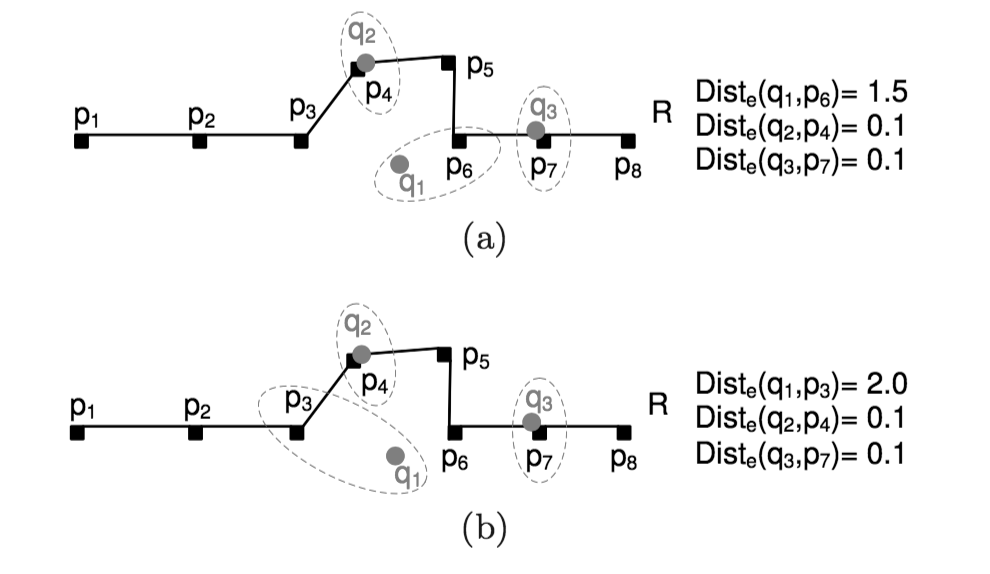
\includegraphics[width=0.7\textwidth]{chapter03/similarity.png}
  \bicaption[fig:3-1]{这里将出现在插图索引中}{查询点与轨迹之间的匹配}{Fig}{Match between query points and trajectory}
\end{figure}

有序查询的相似性计算和无序查询也有区别。给定一组有序的查询点$Q_{o} = \{q_{o1},q_{o2},q_{o3},\cdots, q_{on}\}$和一条已有轨迹$R$,我们通过递归思想为有序查询重新定义相似度方程为$Sim_{o}(Q,R)$,式\ref{eq3-3}。其中$Head(x)$函数代表$x$中的第一个点,例如$Head(Q)$是查询点$q_{1}$;同时$Rest(x)$表示$x$去掉x第一个点之后剩余的部分,例如$Rest(Q)$代表\{$q_{2},q_{3},\cdots, q_{n}$\}。在式\ref{eq3-3}中,通过递归的想法,本文将对$Sim_{o}(Q,R)$的求最大值问题分为对两个子问题的求解,即分别计算$Sim_{o}(Rest(Q),R)$和$Sim_{o}(Q,Rest(R))$的最大值问题。当$Head(Q)$和$Head(R)$的两个轨迹点匹配的时候,我们可以将$e^{-D_{e}(Head(Q), Head(R))}$提前计算并加入当后面计算的$Sim_{o}(Rest(Q),R)$之中。在这种情况下,$Head(R)$需要为下一轮的比较计算继续保留,因为对于$Rest(Q)$中的查询点来说,$Head(R)$依旧有可能成为最佳匹配点。而当当$Head(Q)$和$Head(R)$不匹配的时候时我们则跳过$Head(R)$计算$Sim_{o}(Q,Rest(R))$。这种求解思路类似于动态规划的思路,这也为我们再后面优化过程中通过动态规划的来解决这一问题提供了参考。式\ref{eq3-3}结合了动态时间规整(DTW)利用重复点和最长公共子序列(LCSS)省略不匹配点的优点来计算相似度方程。

\begin{equation} 
\label{eq3-3} 
Sim_{o}(Q,R)= max \left\{  
	\begin{array}{lr}  
    e^{-D_{e}(Head(Q), Head(R))} + Sim_{o}(Rest(Q),R) & \\
    Sim_{o}(Q,Rest(R)) &  
    \end{array}  
\right.  
\end{equation}  

根据相似度方程,本文可以对k最佳连接查询有以下定义3.1.2.:

%\begin{thm}[k最佳连接]
%	给定一组轨迹集合 $T = {R_{1}, R_{2}, R_{3} \cdots, R_{n}}$、一组查询点$Q = {q_{1},q_{2},q_{3},\cdots, q_{n}}$和对应的相似度方程$Sim$,k最佳连接查询则可以从轨迹集合$T$中找到k条轨迹$T'$,满足式\ref{eq3-4}:
%	\begin{equation}
%		\label{eq3-4}
%		Sim(Q,R_{i})_{R_{i} \in T'} \geq Sim(Q,R_{j})_{R_{j} \in T-T'}
%	\end{equation}
%	其中$Sim$根据用户定义选择是否考虑有序性。
%\end{thm}

\theoremstyle{definition}
\begin{definition}
	给定一组轨迹集合 $T = {R_{1}, R_{2}, R_{3} \cdots, R_{n}}$、一组查询点$Q = {q_{1},q_{2},q_{3},\cdots, q_{n}}$和对应的相似度方程$Sim$,k最佳连接查询则可以从轨迹集合$T$中找到k条轨迹$T'$,满足式\ref{eq3-4}。其中$Sim$根据用户定义选择是否考虑有序性。:
	\begin{equation}
		\label{eq3-4}
		Sim(Q,R_{i})_{R_{i} \in T'} \geq Sim(Q,R_{j})_{R_{j} \in T-T'}
	\end{equation}
\end{definition}

\section{相似轨迹查询处理过程}
\label{sec:query processing}

\subsection{问题概述}
\label{sec:problem Forumation}
轨迹数据为一组有序点集,轨迹$R$可以被表示为$R={p_{1}, p_{2}, \cdots, p_{n}}$,其中$p_{i}$是轨迹$R$的在时间顺序上的第$i$个轨迹点。对于本文应用而言,查询点集$Q$被定义为一组点集$Q={q_{1}, q_{2}, \cdots, q_{m}}$,且根据具体情况定义是否有序。在根据上文设计的相似性距离和k最佳连接定义后,我们将我们相似轨迹查询任务等价转化为k最佳连接查询,并产生下面的定义:

\theoremstyle{definition}
\begin{definition}
	给定已有的轨迹数据集$D$,和一条待查询轨迹$R_{q}$。我们通过轨迹简化算法\ref{algo:ts}将待查询轨迹$R_{q}$转换成一组查询点集$Q$。通过k最佳连接查询方法,从轨迹数据集$D$中获取k条轨迹,集合为$D' = {R_{1}, R_{2}, \cdots, R_{k}}$,满足式\ref{eq3-5}。其中$Sim$根据用户定义选择是否考虑有序性。:
	\begin{equation}
		\label{eq3-5}
		Sim(Q,R_{i})_{R_{i} \in D'} \geq Sim(Q,R_{j})_{R_{j} \in D-D'}
	\end{equation}
	我们称$D'$轨迹数据集合为对于轨迹$R_{q}$的k条最相似轨迹查询结果。
\end{definition}

处理上述问题的直观方法可以选择对轨迹集合$D$进行全局搜索,维护一个关键字为相似度大小的优先队列,然后返回结果。但对于系统而言,这样处理数据过于浪费时间。

为解决上述问题,我们首先需要明确我们查询输入的优势在于我们输入的查询点相对于传统的相似轨迹查询方法要小。这是我们能够合理且有效运用空间索引分别对每一个查询点应用近邻查询,并合并查询结果生成k最佳相似轨迹的基本前提。这一方法的搜索复杂度相对于查询点集来说相对恒定。因此,当得出一条轨迹对于查询点集的最近轨迹点便为我们计算该条轨迹与查询点集相似度的上下界提供可能。本文中使用R树索引并搜索近邻的轨迹点,当我们找到关于某个查询点$q$的最近轨迹点$p$,那么包含$p$轨迹点的轨迹一定是离该查询点$q$最近的一条轨迹。

其次在设计搜索框架过程中,我们借鉴\emph{备选和筛选}(candidate generation and refinement)这一思路。这一思路最初提出为在分布式系统中进行k最大数据处理。首先每个子系统的数据按从大到小排列然后并行合并后进行筛选,选出最好的k个结果。这一思路结合k最近邻查询符合本文对算法设计的要求,我们对查询点集$Q$中的每一个点都进行查询并将他们的结果合并生成暂时的轨迹备选集,然后通过筛选的方法选出最相似的k条轨迹。问题的关键在于如何进行轨迹备选集的搜索,以及如何保证k条最相似轨迹的完备性。

本文的相似轨迹查询方法利用R树数据结构,通过简单的k最近邻算法并在其基础上进行有效深度拓展和具体实践优化实现k最佳连接查询以实现相似轨迹查询。表\ref{tab-notations}提供了本文需要的基本符号及其注释。
\\
\begin{table}[!htpb]
  	\centering
		\begin{tabular}{ |p{3cm}||p{9cm}|  }
		\hline
		符号标记 & 符号注释 \\
		\hline
		$N$ & 一条轨迹的轨迹点总数目 \\
		\hline
		$m$ & 一组查询点总数目 \\
		\hline
		$D_{e}(q_{i},p_{j})$ & 点$q_{i}$和点$p_{j}$之间的欧氏距离 \\
		\hline
		$D_{e}(q_{i},p_{j})$ & 点$q_{i}$和点$p_{j}$之间的欧氏距离 \\
		\hline
		$D_{q}(q_{i},R)$ & 点$q_{i}$和轨迹$R$之间的最短距离 \\
		\hline
		$C$ & 轨迹备选集 \\
		\hline
		$\epsilon$ & TBD\\
		\hline
		$r$ & $\lambda$-NeareatNeighbor搜索半径\\
		\hline
		$\rho$ & 轨迹点密度\\
		\hline
		$\xi$ & 查询点$q_{i}$对相似度上界贡献度\\
		\hline
		$\mu,\upsilon$ & 优化搜索权值\\
		\hline
		\end{tabular}
	\bicaption[tab-notations]{出现在表目录的标题}{本文符号列表及其对应注释}{Table}{A list of notations and explanations}
\end{table}
\\

\subsection{生成轨迹备选集}
\label{subsec:candidate-generation}
将预处理的轨迹点存储在R树之中后,我们可以有效地通过k最近邻搜索方法来找到离某一查询点$q$最近的一条轨迹。假设现有一组查询点$Q = \{q_{1},q_{2},\cdots, q_{m}\}$,进行无序的相似轨迹查询。我们首先对这一组查询点中的每一个查询点进行$\lambda NN$查询并得到结果如下:

\begin{align*}
\lambda NN(q_{1}) &= \{p_{1}^{1}, p_{1}^{2}, p_{1}^{3}, \cdots, p_{1}^{\lambda}\}\\ 
\lambda NN(q_{2}) &= \{p_{2}^{1}, p_{2}^{2}, p_{2}^{3}, \cdots, p_{2}^{\lambda}\}\\ 
\cdots\\
\lambda NN(q_{m}) &= \{p_{m}^{1}, p_{m}^{2}, p_{m}^{3}, \cdots, p_{m}^{\lambda}\}
\end{align*}

通过每个查询点根据$\lambda NN$算法生成的结果,我们根据结果中的点生成我们的轨迹备选集。包含$\lambda NN(q_{i})$中至少一个轨迹点的轨迹被加入到轨迹备选子集$C_{i}$中用于之后生成k最佳连接结果。在这一步我们需要保证轨迹备选子集$C_{i}$的基数应该小于等于$\lambda$,因为多个属于$\lambda NN(q_{i})$的轨迹点有可能属于同一条轨迹。之后我们合并所有由$\lambda NN(q_{i})$查询结果得出的轨迹备选子集以获取一个包含$f$条轨迹的轨迹备选集$C$

\begin{equation} 
 C = \bigcup_{i=1}^{m} C_{i} = \{R_{1}, R_{2}, \cdots, R_{f}\} \nonumber
\end{equation}  

对于轨迹备选集$C$中的每一条轨迹$R_{x} (1 \leq x \leq f)$而言,$R_{x}$必须包含至少一个离对应查询点距离在固定范围内的轨迹点。即假使$R_{x}$属于某一轨迹备选子集$C_{i}$($C_{i}$为轨迹备选集$C$的子集),那么$\lambda NN(q_{i})$中的应该包含轨迹$R_{x}$上的一点且$q_{i}$到轨迹$R_{x}$的最短距离是已经计算过的。由于轨迹$R_{x}$和查询点$q_{i}$至少有一组已知的匹配点,则我们可以通过已知匹配点来计算出轨迹备选集中轨迹与查询点集相似度的下界,我们定义为$LB$(lower bound)。

\begin{equation}
	\label{eq3-6}
	LB(R_{x}) = \sum_{1\leq i\leq m \wedge R_{x}\in C_{i}}\bigg( \max_{1\leq j\leq \lambda \wedge p_{i}^{j}\in R_{x}}e^{-D_{e}(q_{i}, p_{i}^{j})}\bigg)
\end{equation}


在计算下界的时候,我们考虑的查询点集为$Q_{matched}$ = \{$q_{i} | 1\leq i\leq m \wedge R_{x} \in C_{i}$\},对于$Q_{matched}$中的查询点来说,他们和轨迹$R_{x}$上的某一个轨迹点在进行k最近邻查询中被计算作为匹配点,即对于查询点$q_{i} \in Q_{matched}$,我们可以找到轨迹上的某一点$p_{i}^{j}$满足$e^{-D_{e}(q_{i}, p_{i}^{j})}$达到最大值,因为在欧氏距离上$q_{i}$与$p_{i}^{j}$最为接近,根据这一点我们可以将式\ref{eq3-6}中的$\max_{1\leq j\leq \lambda \wedge p_{i}^{j}\in R_{x}}e^{-D_{e}(q_{i}, p_{i}^{j})}$等价写成$e_{-D_{q}(q_{i}, R_{x})}$,得出式\ref{eq3-7}

\begin{equation}
	\label{eq3-7}
	LB(R_{x}) = \sum_{1\leq i\leq m \wedge R_{x}\in C_{i}}e^{-D_{q}(q_{i}, R_{x})}
\end{equation} 

显然这个相似度下界值不会大于$\sum_{i=1}^{m} e^{-D_{q}(q_{i}, R(x))}$,因为在计算相似度下界的时候值考虑了与在轨迹$R_{x}$上与某些查询点匹配轨迹点。另一方面,加入轨迹$R_{x}$不属于某个备选轨迹子集$C_{i}$,则轨迹$R_{x}$上任意轨迹点都不会存在于由查询点$q_{i}$得到的k最近邻查询结果$\lambda NN$中。这说明由式\ref{eq3-6}或\ref{eq3-7}定义的相似度下界计算对于式\ref{eq3-2}是成立的。

对于在不属于轨迹备选集$C$中的轨迹($R_{ns} \notin C$),这些轨迹并没有在查询点集进行k最近邻查询中被扫描,他们到查询点$q_{i}$的距离将会小于$p_{i}^{\lambda}$到查询点$q_{i}$的最短距离,即$D_{e}(q_{i}, p_{i}^{\lambda})$。这一发现能让我们计算出所有不属于轨迹备选集的轨迹$R_{ns}$对于查询点集的相似度的上界,我们定义为定义为$UB_{ns}$(upper bound)。

\begin{equation}
	\label{eq3-8}
	UB_{ns} = \sum_{i=1}^{m}e^{-D_{e}(q_{i}, p_{i}^{\lambda})}
\end{equation}

当我们在进行有关空间意义上的数据搜索的时候,剪枝是保证搜索效率的重要手段。相似度的上下界让我们可以设计出针对k最佳连接的剪枝算法以限制搜索空间,提高搜索效率,避免了对整个轨迹数据集或者对不满足条件的轨迹进行多余操作。根据相似度的上下界我们提出下述定理:
\\

\begin{thm}[相似度上下界]
	\label{thm3-1}
	假设对于相似轨迹插叙的k最佳连接算法没有有序性限制,我们可以在对查询点集进行一轮k最近邻查询(k=$\lambda$)之后的轨迹备选集C中,选取一个包含k条轨迹的一个轨迹子集$C'$。当$\min_{R_{x}\in C'}{LB(R_{x})}\geq UB_{us}$这一条件满足时,我们可以从轨迹备选集$C$中获得k条最佳连接轨迹,即k条与查询点集最相似的轨迹。
	\begin{proof}
	首先对于轨迹子集$C'$中的某一条轨迹$R_{a}$($R_{a} \in C'$)而言,轨迹$R_{a}$满足$Sim(Q,R_{a}) \geq LB(R_{a})$。与此同事,对于轨迹备选集$C$之外的轨迹$R_{b}$($R_{b} \notin C$),轨迹$R_{b}$满足$UB_{ns} \geq Sim(Q,R_{b})$。当上述定理成立时,即$\min_{R_{a}\in C'}{LB(R_{a})}\geq UB_{ns}$,我们可以推断出$\forall R_{a}\forall R_{b} \big( R_{a} \in C' \wedge R_{b} \notin C \big)$,$Sim(Q,R_{a}) \geq Sim(Q,R_{b})$成立。这也证明了对于查询点集$Q$得到的k最佳连接的结果轨迹在这个时候应该全部在轨迹备选集$C$中。
	\end{proof}
\end{thm}

需要注意的是定理\ref{thm3-1}中的轨迹子集$C'$不一定全是k最佳连接轨迹的结果,我们只能保证k最佳连接的轨迹在轨迹备选集$C$中。而定理\ref{thm3-1}是我们在进行k最近邻查询而找到k最佳连接轨迹的保证条件。
\\

\subsection{增长型k最近邻查询算法}
\label{subsec:iknn}
在搜索过程中我们需要解决一个关键问题就是$\lambda$的取值问题,$\lambda$值的大小决定了我们的k最佳连接轨迹,即k最相似轨迹是否存在于轨迹备选集$C$中。在定理\ref{thm3-1}中我们的轨迹备选集$C$的基数大小从在很大程度上取决于我们设定的查询$\lambda$值的大小。假如$\lambda$的值我们取的较大,则k最佳连接轨迹基本包含于轨迹备选集$C$内,但这样会造成搜索空间过大的问题。另一方面,$\lambda$过小会使得轨迹备选集$C$不完全包含k最佳连接轨迹,导致搜索的不准确性和错误性。
\\

\begin{algorithm}
%\begin{algorithm}[htp] % 强制定位
\caption{增长型k最近邻查询算法}
\label{algo:iknn}
\begin{algorithmic}[1] %每行显示行号
\Require 相似轨迹查询数目$k$, 查询点集$Q$ % 输入
\Ensure k条最相似轨迹$k$-$Trajs$ % 输出

\State Candidate Set $C$; //初始化轨迹备选集$C$
\State Initialise Upper bound of Similarity $UB_{ns}$; //初始化轨迹相似度上界
\State Initialise Lower bounds $LB[]$, $k-LB[]$; //初始化两个有关相似度下界的数组
\State $\lambda \gets k$ //将k值初始赋值给$\lambda$
\While {true}
	\For{each $q_{i} \in Q$ that $1\leq i\leq m$}
		\State $C_{i}\gets$ trajectories that contains the points in $\lambda$-$NN(q_{i})$;
	\EndFor
	\State $C \gets\bigcup_{i=1}^{m}C_{i}$; //合并轨迹备选子集以生成轨迹备选集C
	\If {$|C| \geq k$}
		\State compute $LB[]$ for all trajectories in $C$; //计算轨迹备选集C中的所有轨迹相似度下界
		\State compute $UB_{ns}$; //计算相似度上界
		\State $k$-$LB[]\gets$ $LB[]$.heapKtop(); //选取相似度下界k个最大值和其对应的轨迹
		\If {$k$-$LB[].min\geq UB_{ns}$} //满足定理\ref{thm3-1}
			\State $k$-$Trajs\gets refine(C)$ //轨迹筛选方法
			\State \textbf{return} $k$-$Trajs$ 
		\EndIf 
	\EndIf
	\State $\lambda\gets\lambda+\Delta\lambda$;
\EndWhile
\end{algorithmic}
\end{algorithm}


为了解决$\lambda$的取值问题,我们尝试通过动态调整$\lambda$值的方法来一步步满足查询结果,这是我们提出\emph{增长型k最近邻查询算法}的基本思想。增长性k最近邻查询算法是基于备选和筛选模式获取备轨迹的高效算法,其大致思想是在算法开始对每一个查询点初步进行k最近邻查询($k=\lambda$,最初$\lambda$可以是任一正整数值)。查询结果如果不满足定理\ref{thm3-1}条件,我们再在$\lambda$值上进行动态增加$\Delta\lambda$,将查询范围从$\lambda$增加到$(\lambda+\Delta\lambda)$,然后我们进行$(\lambda+\Delta\lambda)$最近邻查询。持续这一过程直到我们找到满足定理\ref{thm3-1}条件的$\lambda$值。实现过程伪代码为算法\ref{algo:iknn}所示。


算法\ref{algo:iknn}的具体实现细节如下。通过函数主体首先定义初始化几个中间变量。$while$循环实现增长型k最邻近的每一轮查询。查询中,对查询点集$Q$中的每一个查询点进行k最近邻方法查询,对查询结果中的每一个轨迹点所在的轨迹都加入轨迹备选集$C$。判断轨迹备选集$C$的基数大小是否满足条件。如果满足条件,计算此时归集备选集中所有轨迹的相似度下界大小并用一个数组$LB[]$进行保存,同时计算未在轨迹备选集中的轨迹的相似度上界大小。运用堆排序或优先队列的思想将数组$LB[]$中选取$k$个最大相似度下界及相对应的轨迹。如果\ref{thm3-1}满足,即选出来$k$条轨迹中的最小轨迹相似度下界大于等于未在轨迹备选集中的轨迹相似度上界,则说明我们需要查询的$k$条最相似轨迹已经存在于轨迹备选集$C$中,并且其他未扫描到的轨迹可以忽略不予以计算与检查。
\\

\subsection{轨迹筛选算法}
\label{subsec:refinement}
在增长型k最近邻算法实现过程中,我们利用数组$LB[]$进行堆排序或优先队列获取的k条轨迹相似度下界最大的对应轨迹并不能直接作为我们所需要查询的k条最相似轨迹。第一,轨迹相似度下界并不能直接作为评判轨迹之间相似程度的大小的比较标注;第二,有可能存在多于k条轨迹,他们的相似度下界均大于此时的未在轨迹备选集中的轨迹相似度上界。因此我们需要在增长型k最近邻算法中加入轨迹筛选算法,找到真正满足轨迹相似的k条轨迹。

在增长型k最邻近算法中,我们通过轨迹筛选算法$refine(C)$,对轨迹备选集$C$中的轨迹进行剪枝,去掉不符合条件的轨迹然后再获取k条最相似轨迹。实现轨迹筛选算法,我们仅针对已有的轨迹备选集$C$定义其中轨迹的相似性上界。

\begin{equation}
	\label{eq3-9}
	UB_(R_{x}) = \sum_{1\leq i\leq m \wedge R_{x}\in C_{i}}(\max \limits_{1\leq j\leq \lambda \wedge p_{i}^{j}\in R_{x}}\{e^{-D_{e}(q_{i}, p_{i}^{j})}\}) 
	+ \sum_{1\leq i\leq m \wedge R_{x}\notin C_{i}}(e^{-D_{e}(q_{i}, p_{i}^{\lambda})})
\end{equation}

式\ref{eq3-9}中,轨迹$R_{x} \in C$。对于每一个满足条件${1\leq i\leq m\wedge R_{x}\in  C_{i}}$的查询点$q_{i}$而言,轨迹$R_{x}$到查询点$q_{i}$的的最短距离是在进行k最近邻查询$\lambda$-NN($q_{i}$)中被计算过。因此我们通过这些最短距离匹配点对$<q_{i}, p_{closest}>, p_{closest}\in R_{x}$来计算轨迹备选集中轨迹的相似度上界。对于k最近邻查询结果不包含轨迹$R_{x}$上任意一点的查询点$q_{j}$而言,我们考虑$q_{j}$进行k最近邻查询$\lambda$-NN($q_{i}$)的第$\lambda$个点,即$p_{j}^{\lambda}$。$<q_{j},p_{j}^{\lambda}>$之间的距离肯定比$D_{q}({q_{j},R_{x}})$要近,因此在计算备选集中的轨迹的相似度上界时选择使用$D_{e}(q_{j},p_{j}^{\lambda})$。

\begin{equation} 
\label{eq3-10}
\begin{split}
\forall R_{x}\in C, Sim(Q, R_{x})  & = \sum_{i=1}^{m}(e^{D_{q}(q_{i}, R_{x})})-\sum_{1\leq i\leq m\wedge R_{x}\in C_{i}}(e^{-D_{q}(q_{i}, R_{x})}) -\sum_{1\leq i\leq m\wedge R_{x}\notin C_{i}}(e^{-D_{e}(q_{i}, p_{i}^{\lambda})})\\
 & = \sum_{1\leq i\leq m\wedge R_{x}\notin C_{i}}(e^{D_{q}(q_{i}, R_{x})}-e^{-D_{e}(q_{i}, p_{i}^{\lambda})})\\
 & \leq 0
\end{split}
\end{equation}

式\ref{eq3-10}证明了对于轨迹备选集$C$中的任意一条轨迹而言,$UB$是轨迹相似性的上界值,即$\forall R_{x}\in C, Sim(Q,R_{x}) \leq UB(R_{x})$。

算法\ref{algo:refine}为轨迹筛选算法的实现细节。首先运用优先队列思路,维护一个目前为止的k条最相似轨迹的数组或者队列,并暂时保存其对应的相似度。对轨迹备选集$C$中的每一条轨迹计算其对应的轨迹相似度上界并以此为关键字对轨迹进行从大到小的排序。筛选轨迹算法终止条件当且仅当目前轨迹数组或队列中的最小轨迹相似度大于还未进入过队列的轨迹相似度上界的最大值,此时k条最相似轨迹被准确找出。在循环体中,我们维护轨迹数组或轨迹队列,并在找到一条更匹配或更相似与查询点集的轨迹时更新我们已有的数组和队列。

\begin{algorithm}
%\begin{algorithm}[htp] % 强制定位
\caption{轨迹筛选算法refine(C)}
\label{algo:refine}
\begin{algorithmic}[1] %每行显示行号
\Require 相似轨迹查询数目$k$,轨迹备选集$C$
\Ensure k条最相似轨迹$k$-$Trajs$ % 输出

\State Initialise $k$-$Trajs$ as an array or a priority queue
\State Compute the Upper bound of Similarity, $UB$, for each trajectory in candidate $C$
\State Sort trajectory in candidate $C$ by $UB$ in descending order
\For {$x$ in $range(1, |C|+1)$}
	\State compute $Sim(Q,R_{x})$;
	\If {$x\leq k$}
		\State $k$-$Trajs$.$insert(R_{x},Sim(Q,R_{x}))$;
	\Else 
		\If {$Sim(Q,R_{x})$ > $k$-$Trajs$.$minSim$}
			\State $k$-$Trajs$.removeMinSimTrajectory();
			\State $k$-$Trajs$.$insert(R_{x},Sim(Q,R_{x}))$;
		\EndIf
		\If {$x=|C|+1$ $or$ $k$-$Trajs$.$minSim\geq UB(R_{x+1}$}
			\State \textbf{return} $k$-$Trajs$;
		\EndIf
	\EndIf
\EndFor
\end{algorithmic}
\end{algorithm}


\section{算法优化}
\label{sec:optimization}

\subsection{$\lambda$动态增长优化}
\label{subsec:lambda}
在增长型k最近邻查询算法\ref{algo:iknn}中,对于每一次的k最近邻查询$\lambda$-NN($q_{i}$)而言,搜索范围$\lambda$都是动态增加$\Delta\lambda$,即每一轮循环中,对于查询点集中的每一个查询点$q_{i}$,搜索范围在数目上是相等的。但值得提出的时,在针对地理位置点进行相似轨迹查询这一上下文中,查询点对于结果的重要性并不是完全一致的。主观而言,有些位置点相对于其他位置点来说具有更重要或更优先的查询级别;从算法角度讨论,每个查询点$q$的结果$\lambda$-NN($q$)对于构建轨迹备选集$C$、决定轨迹相似度上下界均有着不同的影响程度。举例来说,对于两个查询点$q_{i}$和$q_{j}$,在$\lambda$相同的情况下,如果$D_{e}(q_{i}, p_{i}^{\lambda}) > D_{e}(q_{j}, p_{j}^{\lambda})$,则对于查询点$q_{i}$所查找的范围更大,即$e^{-D_{e}(q_{i}, p_{i}^{\lambda})} < e^{D_{e}(q_{j}, p_{j}^{\lambda})}$。在式\ref{eq3-8}中,$UB_{ns} = \sum_{i=1}^{m}e^{-D_{e}(q_{i}, p_{i}^{\lambda})}$,我们可以根据结果推出在降低未在备选集中的轨迹相似度上界的过程中,查询点$q_{i}$比查询点$q_{j}$效果更好,更有帮助。在定理3.1.2.中,未在备选集中的轨迹相似度上界越低,则定理条件越容易满足,即增长型k最近邻查询算法可以更快得出结果。我们需要分析$\lambda$对每个查询点搜索的影响来决定如何动态增加搜索范围。首先我们定义每个查询点$q_i$对于$UB_{ns}$的影响为$\xi (q_i)$

\begin{displaymath}
	\xi (q_i) = e^{-D_{e}(q_i,p_i^\lambda)}
\end{displaymath}
显然,当$\xi (q_i)$的值越小时,则相对应的$UB_{ns}$也将越小。接着我们定义$\rho$为某一范围内轨迹点的密度值,定义$r=D_{e}(q_i,p_i^\lambda)$为对查询点$q_i$进行k最近邻查询时的搜索半径。在k最近邻查询这一范围内,我们可以粗略计算出轨迹点的密度值$\rho$等于

\begin{displaymath}
	\rho = \frac{\lambda}{\pi r^{2}}
\end{displaymath}
根据轨迹点密度和搜索半径的关系,我们重写$\xi (q_i)$为

\begin{displaymath}
	\xi (q_i) = e^{-D_{e}(q_i,p_i^\lambda)} = e^{-r} = e^{-\sqrt{\frac{\lambda}{\pi\rho}}}
\end{displaymath}
在这一步,我们的首要目标是明确$\xi (q_i)$影响因子的下降速度与$\lambda$之间的关系,根据$\lambda$的变化所造成的影响赋予查询点$q_1$到$q_m$不同的$\Delta\lambda$变化值,即对于不同的查询点,除了初始第一轮查询之外,之后($\lambda+\Delta\lambda$)的值都是各自生成的。本文将$\xi (q_i)$为关于$\lambda$的微分值$\frac{d\xi}{d\lambda}$的绝对值定义为下降速率$Decay(q_i)$

\begin{equation}
\label{eq3-11}
\frac{d\xi}{d\lambda} = \frac{d}{d\lambda}e^{-\sqrt{\frac{\lambda}{\pi\rho}}} = -\frac{1}{2}(\pi\rho\lambda)^{-\frac{1}{2}}*e^{-\sqrt{\frac{\lambda}{\pi\rho}}}
\end{equation}
根据式\ref{eq3-11},我们可以用$\lambda$和搜索半径$r$来计算轨迹点密度$\rho$,因此可以改写下降速率为

\begin{equation}
\label{eq3-12}
Decay(q_i) = |\frac{d\xi}{d\lambda}| = \frac{r}{2\lambda}e^{-r} 
\end{equation}

根据式\ref{eq3-12},我们可以得知,对于一个固定的$\lambda$值来说,下降速率$Decay(q_i)$会随着搜索半径$r$的不断增长,先初步上升($r\in(0,1]$)后逐渐下降$r\in(1,\infty)$)。我们可以得知在对于查询结果较为稀疏的查询点(即搜索半径$r$较大)在一开始赋予较大的查询权重值。但随着搜过过程的进行,当搜索半径$r$不断增长达到某一个值得时候,一些相对密集的查询点结果会使得其对应的下降速率变大。这一结论使得我们在搜索和查询过程中重点关注查询点结果较为密集的查询点,这样也能使得我们能更快更有效地在每一轮查询之后降低未在轨迹备选集中轨迹的相似度上界值$UB_{ns}$。但随之产生的问题在于,当搜索半径$r$和$\lambda$都足够大的时候,我们下降$UB_{ns}$会因为$\frac{d\xi}{d\lambda}$趋近于0而变得不再有效。

满足定理\ref{thm3-1}需要上下界两个变量对条件的同时满足。因此,在关注未在轨迹备选集中轨迹的相似度上界值$UB_{ns}$对增长型k最近邻查询的影响时,我们可以在加速增长型k最近邻查询算法的时候考虑相似度下界这一因素。当备选集中轨迹的相似度下界$LB$增长越快的时候,定理\ref{thm3-1}也就越容易成立。提高相似度下界$LB$所要面对的问题在于,一条轨迹的相似度下界有可能是源于多个查询点所产生查询结果,并且想要预测在搜索过程中什么时候$\lambda$-NN($q_i$)的结果中的某一点和轨迹上的某一点恰好是同一个点也是不太容易的。换言之,我们问题主要在于定量描述每一个查询点对于相似度下界增长的影响。借此,我们基于每一轮重新查找到的新轨迹数目来定义一个启发式搜索的取回速率$Ratio(q_i)$
\begin{equation}
\label{eq3-13}
Ratio(q_i) = \frac{Number(q_i)}{\Delta\lambda}
\end{equation}

式\ref{eq3-13}中$\Delta\lambda$为当前循环轮次$\lambda$的值与上一轮循环中$\lambda'$值的差值($\lambda > \lambda'$),而$Number(q_i)$表示在当前循环轮次搜索中获取的轨迹数目多少。基本思想在于,轨迹备选集$C$的基数值范会随着搜索过程中新轨迹数目的增长而增长。在这样的归集备选集$C$中,轨迹相似度下界会曾铮的更快,再根据定\ref{thm3-1},我们也更有可能找到目标寻求的k条最相似轨迹。

结合考虑上文所提及的下降速率$Decay(q_i)$和取回速率$Ratio(q_i)$,我们可以对每一个查询点指定对应的$\lambda$查询增长值$\Delta\lambda(q_i)$

\begin{equation}
\label{eq3-14}
\Delta\lambda(q_i) = \gamma\big( \alpha\frac{Decay(q_i)}{\sum_{i=1}^{m}Decay(q_i)} + \beta\frac{Ratio(q_i)}{\sum_{i=1}^{m}Ratio(q_i)} \big)
\end{equation}
式\ref{eq3-14}中,$\alpha$和$\beta$是本文定义的权值,$\gamma$定义为$\gamma = mk2^{r}$ 其中$r$为算法增长型k最近邻查询的当前循环轮次数。这样,我们摈弃原先对每一个查询点都增长相同的$\lambda$值这一处理思路,选择通过式\ref{eq3-14}的方法应用于每一个查询点上以对每个查询的进行不同的$\lambda$增量处理。这样的预先处理会在挖掘出相对重要的轨迹查询点上花费一定时间,但也加速了整个增长型k最近邻查询算法的搜索过程。这样的预处理时间由于优化整个算法过程,因此是可接受的。注意到我们在每一轮$\lambda$增量的总值是

\begin{displaymath}
\sum_{i=1}^{m}\Delta\lambda(q_i)=\gamma\big( \alpha\frac{\sum_{i=1}^{m}Decay(q_i)}{\sum_{i=1}^{m}Decay(q_i)} + \beta\frac{\sum_{i=1}^{m}Ratio(q_i)}{\sum_{i=1}^{m}Ratio(q_i)} \big)=\gamma(\alpha+\beta)
\end{displaymath}
为了保证在每一轮增长型k最近邻查询过程中获取的结果轨迹点数据恒定,我们将$\alpha+\beta$设定为1,其中可以设定$\alpha=\beta=0.5$,这样每一轮我们获取的点的数据为$\gamma$
\\

\subsection{基于动态规划实现有序查询}
\label{subsec:orderquery}
在前文中我们提及查询的有序性和用户指定有关。在进行有序查询的过程中,之前的算法是基于递归进行实现的:通过去不断匹配轨迹和查询点来进行子递归,从而计算出轨迹和有序查询点集之间的相似度大小。但基于递归相似度计算会占用大量的时间。因此在本上,我们通过动态规划的思路来计算某一条轨迹$R$和查询点集$Q$的相似度,借此来优化算法在有序查询中的处理性能。

具体而言,我们借助\ref{algo:dp-sim}算法来处理查询中的有序相似度计算。这里算法的输入为查询点集$Q={q_1,q_2,q_3,\cdots,q_m}$和轨迹$R={p_1,p_2,p_3,\cdots,p_n}$,并通过不断重复或略过轨迹上的点$p_j$来得到最好的匹配结果以计算有序相似度。

\begin{algorithm}
%\begin{algorithm}[htp] % 强制定位
\caption{有序相似度算法dp\_Similarity(Q,R)}
\label{algo:dp-sim}
\begin{algorithmic}[1] %每行显示行号
\Require 查询点集$Q={q_1,q_2,q_3,\cdots,q_m}$,轨迹$R={p_1,p_2,p_3,\cdots,p_n}$
\Ensure 查询点集$Q$和轨迹$R$之间的有序相似度$Sim_{order}(Q,R)$

\State Initialise 2-dimensional array $M[m+1][n+1]$;
\State $M[i][0] \gets 0$ $for$ $1\leq i\leq m$;
\State $M[0][j] \gets 0$ $for$ $1\leq j\leq m$;
\For{$1\leq i\leq m$} 
	\For{$1\leq j\leq n$}
		\If{$e^{-D_{e}(Head(Q),Head(R))} + M[i-1][j] > M[i][j-1]$}//$q_i$和$p_j$匹配
		\State $M[i][j] \gets e^{-D_{e}(Head(Q),Head(R))} + M[i-1][j]$; //重复$p_j$
		\Else 
		\State $M[i][j] \gets M[i][j-1]$; //略过$p_j$
		\EndIf
	\EndFor
	\State \textbf{return} M[m][n];
\EndFor
\end{algorithmic}
\end{algorithm}
算法\ref{algo:dp-sim}中,$M[i][j]$是我们需要解决查询问题的子问题的有序相似度,即$Sim_{order}(\{q_1,q_2,q_3,\cdots,q_i\}, \{p_1,p_2,p_3,\cdots,p_j\})$。对于动态规划思路而言,当我们获取到$M[i-1][j]$和$M[i][j-1]$的值时,我们可以通过比较$e^{-D_{e}(Head(Q),Head(R))} + M[i-1][j]$和$M[i][j-1]$的值来决定$M[i][j]$的最大值。如果值$e^{-D_{e}(Head(Q),Head(R))} + M[i-1][j]$较大,我们可以得出目前的一对匹配点对为$<p_i, p_j>$,并令$M[i][j] = e^{-D_{e}(Head(Q),Head(R))} + M[i-1][j]$,反之,我们略过对$p_j$的目前和之后匹配,并令$M[i][j]=M[i][j-1]$。这一动态规划的思路自底向上的解决了$M[i][j]$的求值问题,其中$m$为查询点集的基数大小而$n$为轨迹点数目。在算法最后通过范围二维数组中的值来表示查询点集$Q$和轨迹$R$之前有序相似度。算法的复杂性为$O(mn)$,在具体应用中由于$m$的值相对于$n$来说普遍较小,所以我们可以将算法复杂性近似看成是线性的。

之后的问题在于如何将有序相似度与增长型k最近邻查询算法结合。首先,对于轨迹备选集$C$中的一条轨迹$R$而言,$R\in C$,轨迹$R$中的某些轨迹点存在于增长型k最近邻查询过程中的某一个或者几个$\lambda$-$NN$结果中,我们定义这些轨迹点为$R'$,显然$R' \subseteq R$,即

\begin{displaymath}
R' = \{p_i | p_i \in R \wedge p_i \in\bigcup_{j=1}^{m}\lambda -NN(q_j)\}
\end{displaymath}

基于有序查询,我们可以得出

\begin{equation}
\label{eq3-15}
Sim_{order}(Q, R) \geq Sim_{order}(Q, R')
\end{equation}
证明式\ref{eq3-15}可以依据反证法:假设$Sim_{order}(Q, R) < Sim_{order}(Q, R')$,其中$Q$和$R'$之间的匹配点对位$\{<q_1, p(\varphi_1)>,<q_2, p(\varphi_2)>,\cdots,<q_m, p(\varphi_m)>\}$,其中$p(\varphi_i) \in R'$,根据有序相似度的定义,$Sim_{order}(Q,R')=\sum_{i=1}^{m}e^{-D_{e}(q_i, p(\varphi_i))}$,由于$R' \subseteq R$,即有$p(\varphi_i) \in R$,那么$sum_{i=1}^{m}e^{-D_{e}(q_i, p(\varphi_i))}$对于$Sim_{order}(Q,R)$也是成立的,则$Sim_{order}(Q,R)$至少大于等于$Sim_{order}(Q,R')$,与假设矛盾。

因此,我们重新修改我们相似性的上下界以使他们使用于有序查询的情况。根据式\ref{eq3-15},我们将相似性的下界通过$R'$上所获取的点来定义;对于相似性的上界我们仅针对轨迹备选集$C$中的轨迹$R_c$ $R_c \in C$来定义

\begin{equation}
\label{eq3-16}
\begin{split}
LB_{order}(R) & = Sim_{order}(Q, R') = dp\_Similarity(Q,R')\\
UB_{order}(R_c) & = LB_{order}(R_c) + \sum_{1\leq i\leq m\wedge R_c\notin C_i}\big( e^{-D_{e}(q_i, p_i^\lambda)} \big)
\end{split}
\end{equation}

根据式\ref{eq3-16}将相似度上下界从无序的定义改成有序的定义,则可以在增长型k最近邻查询中加入有序查询限制,即根据查询点集的查询顺序查询最相似的k的轨迹。


%# -*- coding: utf-8-unix -*-
%%==================================================
%% chapter03.tex for SJRU Master Rhesis
%% implementation2
%%==================================================
%\bibliographystyle{sjtu2}%[此处用于每章都生产参考文献]

\theoremstyle{definition}
\newtheorem{definition}{定义}[section]

\chapter{相似轨迹查询方法实现}
\label{chap:implementation}

\section{相似轨迹查询问题描述}
\label{sec:question describe}
相似轨迹查询传统意义上是根据一条已有历史轨迹,在轨迹数据库中查询出与这一条轨迹在地理位置上形状相似的一条或多条轨迹。在本文中,我们将输入轨迹进一步简化为一组轨迹查询点集$Q$。$Q$在地理位置上保留轨迹原有的形状,通过对点集$Q$进行\emph{k最佳连接}查询,从轨迹数据库$D$中得出k条最相似的轨迹集合$T'$作为输出。由于系统设计与用户的交互,性能指标方面查询结果应满足高效、实时且具有良好的准确性。

\section{k最佳连接定义}
\label{sec:k-bct}
一个轨迹数据库中存储了大量的原始车载GPS轨迹或是已经预处理过的车载GPS轨迹。这里的轨迹由一系列的地理位置点组成$\{p_{1},p_{2},p_{3},\cdots, p_{m}\}$,其中$p_{i}$ $1\leq i \leq m$代表一个由经度和维度构成的地理位置点而$m$代表轨迹中点的数目。本文所定义的k最佳连接查询(k Best-Connected Rrajectory Query)的输入由一组查询点$Q$组成。$q_{j}$ $1 \leq j \leq n$和$p_{i}$定义相同,其中n是查询点的数目。这里用户可以选择选择是否在查询中指定轨迹连接依照查询点的先后顺序,即是否选择查询有序性。若选择查询有序性,则查询点集$Q$为认为是从$q_{1}$到$q_{m}$有序点集。
\begin{displaymath}
	Q = \{q_{1},q_{2},q_{3},\cdots, q_{n}\}
\end{displaymath}

在搜索最好连接轨迹这一上下文中,相似度方程的定义需要和传统方法有所不同,在这里我们将相似度方程定义为一条轨迹连接查询点的好坏程度。因此,本文首要考虑一条轨迹到每一个查询点的距离,我们简要定义距离一个查询点$q_{i}$到一条轨迹$R=\{p_{1},p_{2},p_{3},\cdots, p_{m}\}$的距离为$D_{q}$,即

\begin{equation}
	\label{eq3-1}
	D_{q}(q_{i}, R) = \min_{p_{j} \in R} \{D_{e}(q_{i}, p_{j})\} 
\end{equation}

式\ref{eq3-1}中,$D_{e}(q_{i}, p_{j})$是指查询点$q_{i}$和轨迹点$p_{j}$之间的欧氏距离,因此通常意义上相似度距离$D_{q}$代表从查询点$q_{i}$到轨迹上任一一点距离的最短距离。当我们找到轨迹上一点$p_{j}$是离查询点$q_{i}$的最短距离点时,我们将$<q_{i},p_{j}>$作为最短匹配点对。在无序查询点击中,我们定义查询点集$Q$和轨迹$R$之间的相似度为$Sim(Q,R)$。

\theoremstyle{definition}
\begin{definition}
	轨迹$R={p_{1}, p_{2}, \cdots, p_{n}}$而查询点为$q$,$<q, p_{i}>$表示一组匹配点对。对于$\forall p_{i} \neq p_{j}$, $d_{e}(p_{i}, q)\leq d_{e}(p_{j}, q)$,那么$<p_{i}, q>$是轨迹$R$到查询点$q$的最短匹配点对。
\end{definition}

\begin{equation}
	\label{eq3-2}
	Sim(Q,R) = \sum_{i=1}^{n} \emph{e}^{-D_{q}(q_{i}, R)}
\end{equation}

式\ref{eq3-2}将每个查询点对$Sim(Q,R)$的贡献值通过自然对数去反得以体现,即根据自然函数的单调性,查询点离轨迹越近,则$-D_{q}(q_{i}, R)$越大,以自然对数为底取幂的值也越大,最后使得$Sim(Q,R)$的值也越大。从用户人为角度和地理语义角度上看,一条轨迹与所有的查询点被定义为相似当且仅当这条轨迹和所有的查询点都十分接近。

图\ref{similarity}通过距离说明查询点和轨迹之间的匹配关系。如图\ref{similarity}(a)所示,查询点$q_{1}$、$q_{2}$和$q_{3}$分别与轨迹R上的轨迹点$p_{6}$、$p_{4}$和$p_{7}$最近匹配,根据式\ref{eq3-2}可以得出,$Sim(Q,R) = \emph{e}^{-D_{q}(q_{1}, p_{6})} + \emph{e}^{-D_{q}(q_{2}, p_{4})} + \emph{e}^{-D_{q}(q_{3}, p_{7})} = \emph{e}^{-1.5}+ \emph{e}^{-0.1} + \emph{e}^{-0.1}$。

另一方面,选择查询点和轨迹之前进行有序查询时,顺序性是需要在查询过程中予以考虑。对于查询点$q_{i}$而言,最近匹配点或许并不在是距离上最近的轨迹点$p_{j}$。因此,相似度方程在此步骤中应该适当调整。我们再借用图\ref{similarity}\cite{chen2010searching}予以说明。假设以下用户场景:用户希望查询出一条以$q_{1} \rightarrow q_{2} \rightarrow q_{3}$为顺序的相似轨迹,显然图\ref{similarity}(a)中的顺序并不再符合用户需求。实际的有序查询结果顺序如图\ref{similarity}(b)是$p_{3} \rightarrow q_{4} \rightarrow q_{7}$。在考虑有序性的相似查询规程中,我们的目标是在保持查询有序性的同时追求每一对匹配点对相似度的最大贡献值,即从图\ref{similarity}(b)可以看出$<q_{1},p_{3}>, <q_{2},p_{4}>, <q_{3},p_{7}>$这样的三对匹配点是所有有序匹配对中使得相似度最大的情况。

\begin{figure}[!htp]
  \centering
  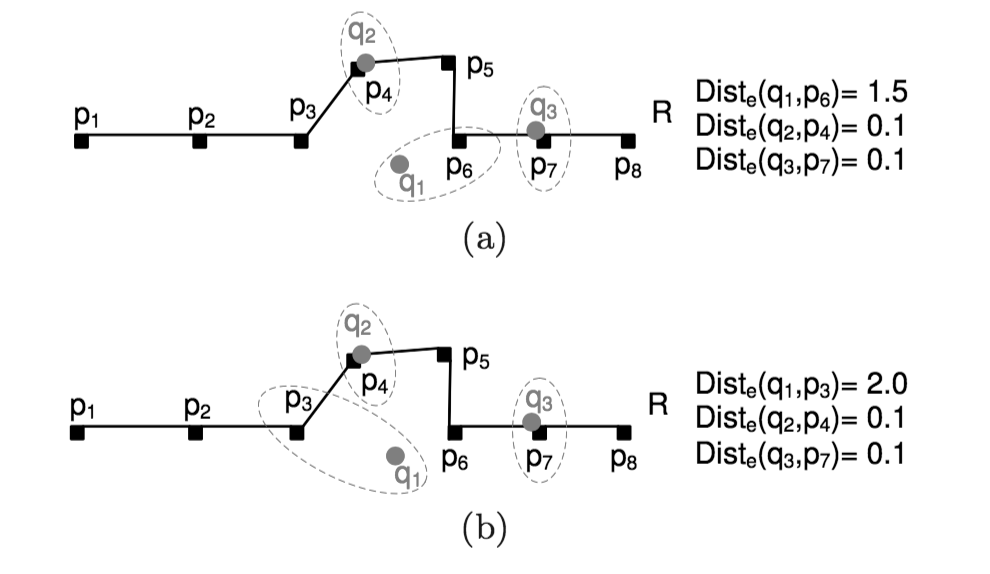
\includegraphics[width=0.7\textwidth]{chapter03/similarity.png}
  \bicaption[similarity]{查询点与轨迹点之间的匹配}{查询点与轨迹点之间的匹配}{Fig}{Match between query points and trajectory point}
\end{figure}

有序查询的相似性计算和无序查询也有区别。给定一组有序的查询点$Q_{o} = \{q_{o1},q_{o2},q_{o3},\cdots, q_{on}\}$和一条已有轨迹$R$,我们通过递归思想为有序查询重新定义相似度方程为$Sim_{o}(Q,R)$,式\ref{eq3-3}。其中$Head(x)$函数代表$x$中的第一个点,例如$Head(Q)$是查询点$q_{1}$;同时$Rest(x)$表示$x$去掉x第一个点之后剩余的部分,例如$Rest(Q)$代表\{$q_{2},q_{3},\cdots, q_{n}$\}。在式\ref{eq3-3}中,通过递归的想法,本文将对$Sim_{o}(Q,R)$的求最大值问题分为对两个子问题的求解,即分别计算$Sim_{o}(Rest(Q),R)$和$Sim_{o}(Q,Rest(R))$的最大值问题。当$Head(Q)$和$Head(R)$的两个轨迹点匹配的时候,我们可以将$e^{-D_{e}(Head(Q), Head(R))}$提前计算并加入当后面计算的$Sim_{o}(Rest(Q),R)$之中。在这种情况下,$Head(R)$需要为下一轮的比较计算继续保留,因为对于$Rest(Q)$中的查询点来说,$Head(R)$依旧有可能成为最佳匹配点。而当当$Head(Q)$和$Head(R)$不匹配的时候时我们则跳过$Head(R)$计算$Sim_{o}(Q,Rest(R))$。这种求解思路类似于动态规划的思路,这也为我们再后面优化过程中通过动态规划的来解决这一问题提供了参考。式\ref{eq3-3}结合了动态时间规整(DTW)利用重复点和最长公共子序列(LCSS)省略不匹配点的优点来计算相似度方程。

\begin{equation} 
\label{eq3-3} 
Sim_{o}(Q,R)= max \left\{  
	\begin{array}{lr}  
    e^{-D_{e}(Head(Q), Head(R))} + Sim_{o}(Rest(Q),R) & \\
    Sim_{o}(Q,Rest(R)) &  
    \end{array}  
\right.  
\end{equation}  

根据相似度方程,本文可以对k最佳连接查询有以下定义3.1.2.:

\theoremstyle{definition}
\begin{definition}
	给定一组轨迹集合 $T = {R_{1}, R_{2}, R_{3} \cdots, R_{n}}$、一组查询点$Q = {q_{1},q_{2},q_{3},\cdots, q_{n}}$和对应的相似度方程$Sim$,k最佳连接查询则可以从轨迹集合$T$中找到k条轨迹$T'$,满足式\ref{eq3-4}。其中$Sim$根据用户定义选择是否考虑有序性。:
	\begin{equation}
		\label{eq3-4}
		Sim(Q,R_{i})_{R_{i} \in T'} \geq Sim(Q,R_{j})_{R_{j} \in T-T'}
	\end{equation}
\end{definition}

在进行有序查询的过程中,之前的算法是基于递归进行实现的:通过去不断匹配轨迹和查询点来进行子递归,从而计算出轨迹和有序查询点集之间的相似度大小。但基于递归相似度计算会占用大量的时间。因此在本上,我们通过动态规划的思路来计算某一条轨迹$R$和查询点集$Q$的相似度,借此来优化算法在有序查询中的处理性能。

\begin{algorithm}
%\begin{algorithm}[htp] % 强制定位
\caption{有序相似度算法dp\_Similarity(Q,R)}
\label{algo:dp-sim}
\begin{algorithmic}[1] %每行显示行号
\Require 查询点集$Q={q_1,q_2,q_3,\cdots,q_m}$,轨迹$R={p_1,p_2,p_3,\cdots,p_n}$
\Ensure 查询点集$Q$和轨迹$R$之间的有序相似度$Sim_{order}(Q,R)$
\State Initialise 2-dimensional array $M[m+1][n+1]$;
\State $M[i][0] \gets 0$ $for$ $1\leq i\leq m$;
\State $M[0][j] \gets 0$ $for$ $1\leq j\leq m$;
\For{$1\leq i\leq m$} 
	\For{$1\leq j\leq n$}
		\If{$e^{-D_{e}(Head(Q),Head(R))} + M[i-1][j] > M[i][j-1]$}//$q_i$和$p_j$匹配
		\State $M[i][j] \gets e^{-D_{e}(Head(Q),Head(R))} + M[i-1][j]$; //重复$p_j$
		\Else 
		\State $M[i][j] \gets M[i][j-1]$; //略过$p_j$
		\EndIf
	\EndFor
	\State \textbf{return} M[m][n]$\setminus n$;
\EndFor
\end{algorithmic}
\end{algorithm}

假设$M[i][j]$是我们需要解决查询问题的子问题的有序相似度,即$Sim_{order}(\{q_1,q_2,q_3,\cdots,q_i\}$, $\{p_1,p_2,p_3,\cdots,p_j\})$。对于动态规划思路而言,当我们获取到$M[i-1][j]$和$M[i][j-1]$的值时,我们可以通过比较$e^{-D_{e}(Head(Q),Head(R))} + M[i-1][j]$和$M[i][j-1]$的值来决定$M[i][j]$的最大值。如果值$e^{-D_{e}(Head(Q),Head(R))} + M[i-1][j]$较大,我们可以得出目前的一对匹配点对为$<p_i, p_j>$,并令$M[i][j] = e^{-D_{e}(Head(Q),Head(R))} + M[i-1][j]$,反之,我们略过对$p_j$的目前和之后匹配,并令$M[i][j]=M[i][j-1]$。由于历史轨迹点的数目各不相同,对于重复使用的点,我们需要将相似度计算结果正则化以符合实际。

这一动态规划的思路自底向上的解决了$M[i][j]$的求值问题,其中$m$为查询点集的基数大小而$n$为轨迹点数目。在算法最后通过范围二维数组中的值来表示查询点集$Q$和轨迹$R$之前有序相似度。算法的复杂性为$O(mn)$,在具体应用中由于$m$的值相对于$n$来说普遍较小,所以我们可以将算法复杂性近似看成是线性的。

\section{相似轨迹查询处理过程}
\label{sec:query processing}

\subsection{算法变量符号定义及解释}
\label{subsec:algorithm-definition-explanation}
表\ref{tab-notations}提供了本文本章节之后所涉及的基本符号及其注释。

\begin{table}[!htpb]
  	\centering
		\begin{tabular}{ |p{1.5cm}||p{5.5cm}|p{1.5cm}||p{5.5cm}| }
		\hline
		符号标记 & 符号注释 & 符号标记 & 符号注释\\
		\hline
		$N$ & 一条轨迹的轨迹点总数目 & $m$ & 一组查询点总数目\\
		\hline
		$D_{e}(q_{i},p_{j})$ & 点$q_{i}$和点$p_{j}$之间的欧氏距离 & $C$ & 轨迹备选集 \\
		\hline
		$D_{e}(q_{i},p_{j})$ & 点$q_{i}$和点$p_{j}$之间的欧氏距离 & $\epsilon$ & 搜索范围阈值\\
		\hline
		$D_{q}(q_{i},R)$ & 点$q_{i}$和轨迹$R$之间的最短距离 & $\rho$ & 轨迹点密度 \\
		\hline
		$r$ & $\lambda$-NeareatNeighbor搜索半径 & $\xi$ & 查询点$q_{i}$对相似度上界贡献\\
		\hline
		$\mu,\upsilon$ & 优化搜索权值 & $UB_{ns}$ & 未在备选集中轨迹的相似度上界\\
		\hline
		$LB$ & 备选集中轨迹的相似度下界 & & \\
		\hline
		\end{tabular}
	\bicaption[tab-notations]{公式符号列表及其对应注释}{本文符号列表及其对应注释}{Table}{A list of notations and explanations}
\end{table}


\subsection{相似轨迹查询问题概述}
\label{sec:problem Forumation}
轨迹数据为一组有序点集,轨迹$R$可以被表示为$R={p_{1}, p_{2}, \cdots, p_{n}}$,其中$p_{i}$是轨迹$R$的在时间顺序上的第$i$个轨迹点。对于本文应用而言,查询点集$Q$被定义为一组点集$Q={q_{1}, q_{2}, \cdots, q_{m}}$,且根据具体情况定义是否有序。在根据上文设计的相似性距离和k最佳连接定义后,我们将我们相似轨迹查询任务等价转化为k最佳连接查询,并产生下面的定义:

%\theoremstyle{definition}
\begin{definition}
	给定已有的轨迹数据集$D$,和一条待查询轨迹$R_{q}$。我们通过轨迹简化算法\cite{visvalingam1990douglas,chen2009trajectory}将待查询轨迹$R_{q}$转换成一组查询点集$Q$。通过k最佳连接查询方法,从轨迹数据集$D$中获取k条轨迹,集合为$D' = {R_{1}, R_{2}, \cdots, R_{k}}$,满足式\ref{eq3-5}。其中$Sim$根据用户定义选择是否考虑有序性。:
	\begin{equation}
		\label{eq3-5}
		Sim(Q,R_{i})_{R_{i} \in D'} \geq Sim(Q,R_{j})_{R_{j} \in D-D'}
	\end{equation}
	我们称$D'$轨迹数据集合为对于轨迹$R_{q}$的k条最相似轨迹查询结果。
\end{definition}

\subsection{相似轨迹查询算法实现}
\label{subsec:algorithm implementation}

\begin{figure}[!htp]
  \centering
  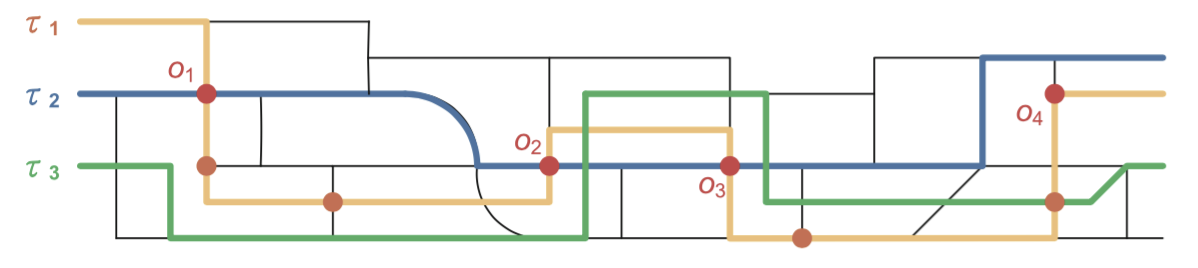
\includegraphics[width=0.8\textwidth]{chapter03/similar-search.png}
  \bicaption[fig:similar-search]{基于位置点的相似轨迹查询}{基于位置点的相似轨迹查询\cite{shang2014personalized}}{Fig}{Search similar trajectory by location points}
\end{figure}

如图\ref{fig:similar-search}\cite{shang2014personalized}所示,本文所实现的相似轨迹查询算法主要为针对地理位置点集的轨迹搜索算法\cite{qi2015efficient}。将轨迹数据按特定需求分类索引在R树数据结构上后,该相似轨迹查询算法在轨迹点k最近邻查询算法\cite{roussopoulos1995nearest}基础上,实现了增长型k最近邻查询算法\cite{chen2010searching},结合备选和筛选(candidate-refinement)的剪枝思路\cite{tang2011retrieving},通过轨迹相似度上界与下界对搜索空间进行优化处理,以满足空间搜索算法的高效性和准确性。

在这里,轨迹相似度上界与下界所满足的搜索剪枝关系用定理\ref{thm:similarity-bound}描述

\begin{thm}[相似度上下界]
	\label{thm:similarity-bound}
	假设对于相似轨迹插叙的k最佳连接算法没有有序性限制,我们可以在对查询点集进行一轮k最近邻查询(k=$\lambda$)之后的轨迹备选集C中,选取一个包含k条轨迹的一个轨迹子集$C'$。当$\min_{R_{x}\in C'}{LB(R_{x})}\geq UB_{us}$这一条件满足时,我们可以从轨迹备选集$C$中获得k条最佳连接轨迹,即k条与查询点集最相似的轨迹。
	\begin{proof}
	首先对于轨迹子集$C'$中的某一条轨迹$R_{a}$($R_{a} \in C'$)而言,轨迹$R_{a}$满足$Sim(Q,R_{a}) \geq LB(R_{a})$。与此同事,对于轨迹备选集$C$之外的轨迹$R_{b}$($R_{b} \notin C$),轨迹$R_{b}$满足$UB_{ns} \geq Sim(Q,R_{b})$。当上述定理成立时,即$\min_{R_{a}\in C'}{LB(R_{a})}\geq UB_{ns}$,我们可以推断出$\forall R_{a}\forall R_{b} \big( R_{a} \in C' \wedge R_{b} \notin C \big)$,$Sim(Q,R_{a}) \geq Sim(Q,R_{b})$成立。这也证明了对于查询点集$Q$得到的k最佳连接的结果轨迹在这个时候应该全部在轨迹备选集$C$中。
	\end{proof}
\end{thm}

%\begin{algorithm}
%\caption{相似轨迹查询算法}
%\label{algo:iknn}
%\begin{algorithmic}[1] %每行显示行号
%\Require 相似轨迹查询数目$k$, 查询点集$Q$ % 输入
%\Ensure k条最相似轨迹$k$-$Trajs$ % 输出
%\State Candidate Set $C$; //初始化轨迹备选集$C$
%\State Initialise $UB_{ns}$ $LB[]$, $k$-$LB[]$ ; //初始化轨迹相似度上界和相似度下界
%\State $\lambda \gets k$ //将k值初始赋值给$\lambda$
%\While {true}
%	\For{each $q_{i} \in Q$ that $1\leq i\leq m$}
%		\State $C_{i} \gets$ trajectories that contains the points in $\lambda$-$NN(q_{i})$;
%	\EndFor
%	\State $C \gets\bigcup_{i=1}^{m}C_{i}$; //合并轨迹备选子集以生成轨迹备选集C
%	\If {$|C| \geq k$}
%		\State compute $LB[]$ for all trajectories in $C$; //计算轨迹备选集C中的所有轨迹相似度下界
%		\State compute $UB_{ns}$; //计算相似度上界
%		\State $k$-$LB[]\gets$ $LB[]$.heapKtop(); //选取相似度下界k个最大值和其对应的轨迹
%		\If {$k$-$LB[].min\geq UB_{ns}$}
%			\State $k$-$Trajs\gets refine(C)$ //轨迹筛选方法
%			\State \textbf{return} $k$-$Trajs$ 
%		\EndIf 
%	\EndIf
%	\State $\lambda\gets\lambda+\Delta\lambda$;
%\EndWhile
%\end{algorithmic}
%\end{algorithm}


算法\ref{algo:iknn}{\cite{chen2010searching}}大致流程如图\ref{fig:iknn-flowchart}。通过函数主体首先定义初始化几个中间变量。$while$循环实现增长型k最邻近的每一轮查询。查询中,对查询点集$Q$中的每一个查询点进行k最近邻方法查询,对查询结果中的每一个轨迹点所在的轨迹都加入轨迹备选集$C$。判断轨迹备选集$C$的基数大小是否满足条件。如果满足条件,计算此时归集备选集中所有轨迹的相似度下界大小并用一个数组$LB[]$进行保存,同时计算未在轨迹备选集中的轨迹的相似度上界大小。运用堆排序或优先队列的思想将数组$LB[]$中选取$k$个最大相似度下界及相对应的轨迹。如果\ref{thm:similarity-bound}满足,即选出来$k$条轨迹中的最小轨迹相似度下界大于等于未在轨迹备选集中的轨迹相似度上界,则说明我们需要查询的$k$条最相似轨迹已经存在于轨迹备选集$C$中,并且其他未扫描到的轨迹可以忽略不予以计算与检查。

%\begin{figure}[!htp]
%  \centering
%  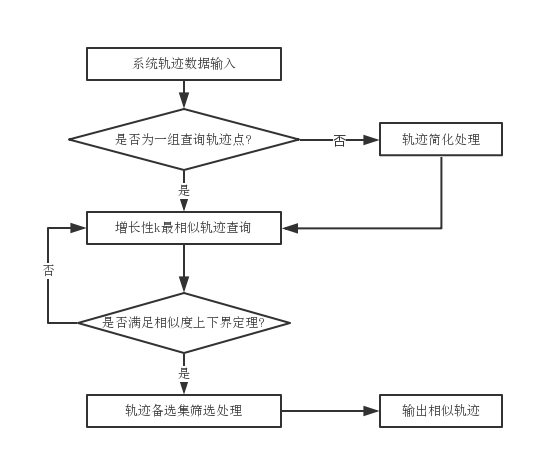
\includegraphics[width=0.8\textwidth]{chapter03/iknn-flowchart.png}
%  \bicaption[fig:iknn-flowchart]{相似轨迹查询算法流程图}{相似轨迹查询算法流程图}{Fig}{Searching algorithm flow chart}
%\end{figure}

\begin{figure}[!htp]
    \centering
    \resizebox{10cm}{!}{
\begin{tikzpicture}[node distance=2cm]

	\node (input) [startstop,font=\bf,fill=green!20] {输入轨迹数据类型判断};
	\node (input_judge) [decision, below of=input,yshift=-0.5cm,aspect=2.5,fill=red!20] {是否为用户指定一组轨迹点集?};
	\node (ts) [process, right of=input_judge,xshift=5cm] {轨迹简化};
	\node (iknn) [process, below of=input_judge,yshift=-0.5cm]{增长型k相似轨迹查询};
	\node (bound_judge) [decision, below of=iknn,yshift=-0.5cm,aspect=2.5,fill=red!20]{是否满足相似度上下界条件?};
	\node (refinement)[process, below of=bound_judge,yshift=-0.5cm]{备选轨迹集筛选};
	\node (output)[startstop, below of=refinement,font=\bf,fill=green!20]{k条最相似轨迹输入};
	

	\draw [arrow] (input) -- (input_judge);
	\draw [arrow] (input_judge) -- node[anchor=south]{否}(ts);
	\draw [arrow] (input_judge) -- node[anchor=west]{是}(iknn);
	\draw [arrow] (ts) |- (iknn);
	\draw [arrow] (iknn) -- (bound_judge);
	\draw [arrow] (bound_judge.west) |- node[anchor=south]{否}(iknn.west);
	\draw [arrow] (bound_judge.south) -- node[anchor=west]{是}(refinement.north);
	\draw [arrow] (refinement) -- (output);
\end{tikzpicture}

}
    \bicaption[fig:iknn-flowchart]{相似轨迹查询算法流程图}{相似轨迹查询算法流程图}{Fig}{Searching algorithm flow chart}
\end{figure}


%%%%%%%%%%


\section{分布式相似轨迹查询算法实现}
\label{sec:distributed algo}
在之前的工作描述中,我们对于相似轨迹查询的实现总会提及查询点集的数目相对较少这一前提。对于单机处理而言,如果将一整条轨迹的轨迹数据点作为输入或者查询点集过多,由于增长型k最近邻查询会对每一个查询点都进行$\lambda$-NN的搜索处理,因此整个相似轨迹的查询过程会显得相对缓慢。但有些时候,将一条轨迹作为相似轨迹查询的输入的确更简单且更人性化\cite{shang2014personalized}。在硬件设置对算法性能的约束下,借助基于地理位置点的轨迹简化方法,我们可以对前一章所涉及的相似轨迹查询方法通过加入\emph{Spark}分布式集群处理的手段,做到以一条轨迹(或数量更多的查询点)为输入的相似轨迹查询操作。具体实现思路在于,通过基于地理位置点的轨迹简化方法将一条轨迹简化为一组数量相对于单机查询要多的查询点集;然后将查询点通过分布式集群操作分配给各个子节点来进行相对于各集群节点的相似轨迹查询操作,各个子节点通过访问HDFS获取轨迹数据和轨迹R树索引;最后将结果以轨迹为关键字,以相似度为权值进行求和,选择相似度和最高的k条轨迹作为查询结果。


\subsection{Spark分布式相似轨迹查询}
\label{subsec:distributed similar}
\emph{Spark}集群环境使得我们可以将代码分发给各个工作节点使他们处理对数据集相同的操作,这为分布式搜索相似轨迹提供了实现的基础。单机实现相似轨迹搜索为保证运行性能,给定的输入集查询点需要保证数量在某一程度上相对较小。但对于分布式处理而言,这一约束可以通过集群集计算处理予以取消。给定一条原始轨迹$Traj$,我们可以先通过基于地理位置点的轨迹简化在保留轨迹形状和轨迹中的重要位置点的同时,一定程度上减少轨迹数目。事实上,如果集群设备性能较好,我们可以略去集群计算相似轨迹前对轨迹简化这一步骤。由于本文实验设备限制,通过在集群处理前的轨迹简化能在保证结果正确性的过程中,稳定处理性能。因此,我们将轨迹简化作为集群计算前的预处理过程。

\begin{figure}[!htp]
  \centering
  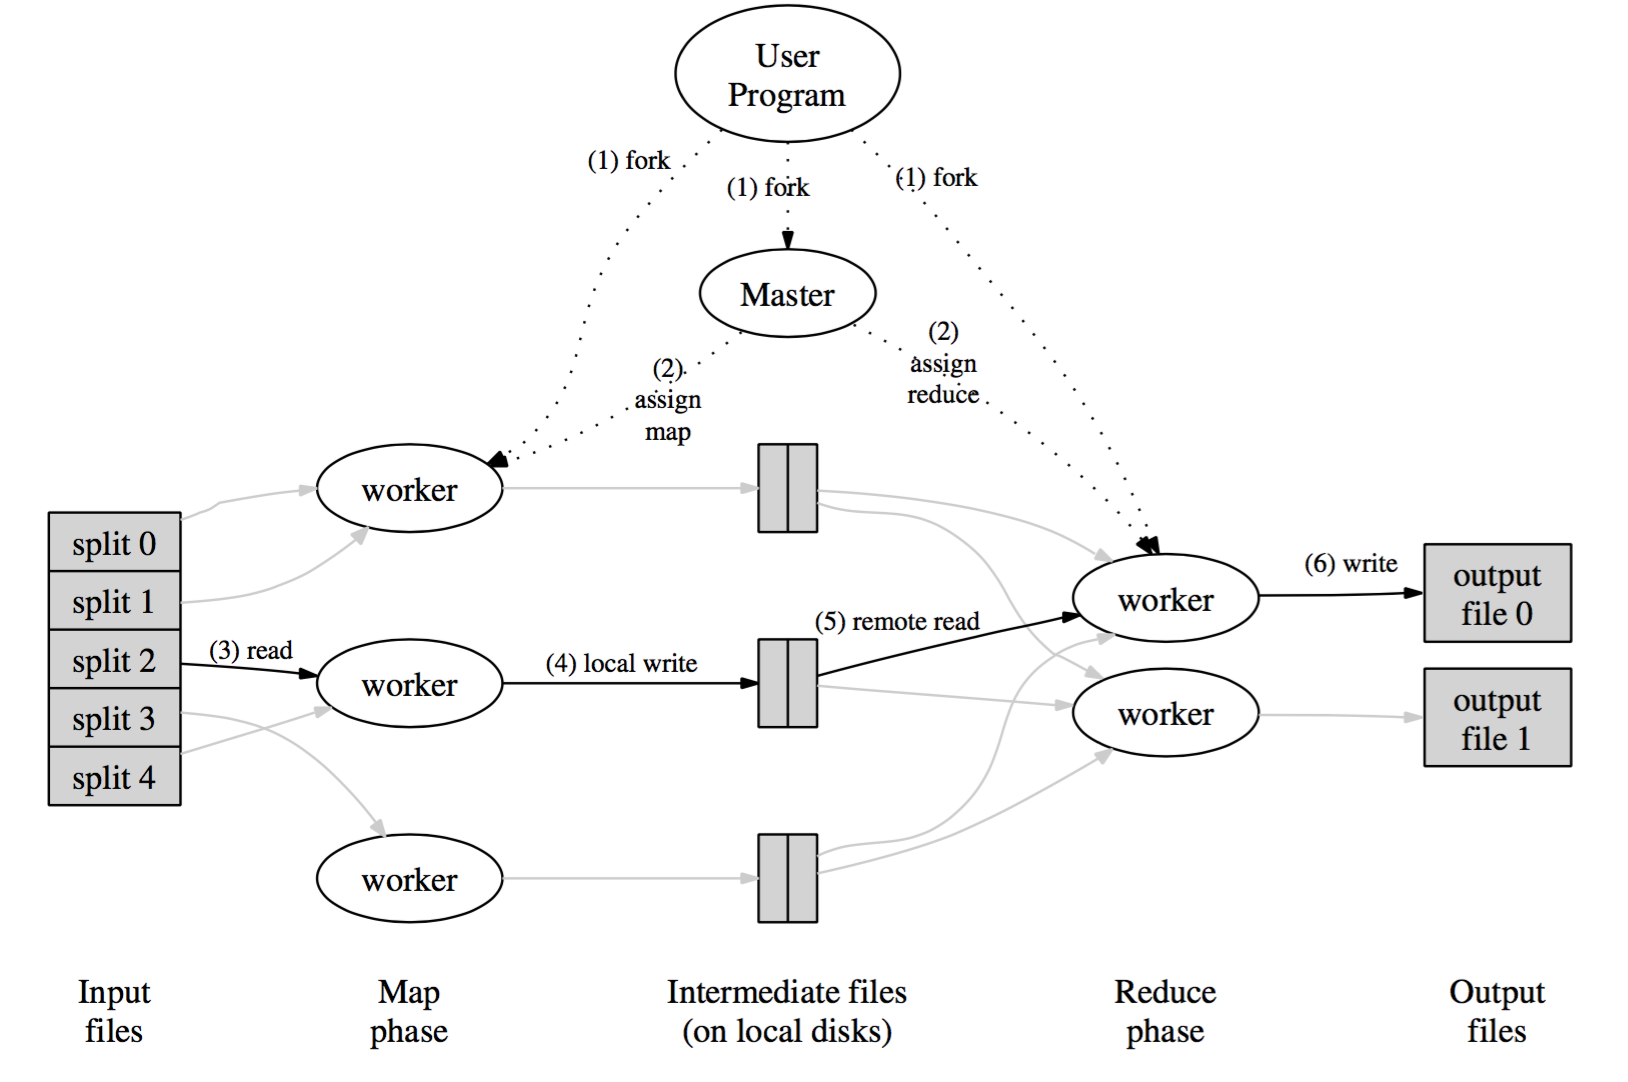
\includegraphics[width=0.8\textwidth]{chapter04/distributed.png}
  \bicaption[fig:distributed]{Spark分布式相似轨迹查询流程}{Spark分布式相似轨迹查询流程\cite{dean2008mapreduce}}{Fig}{The flow of Spark distributed search similar trajectories}
\end{figure}

图\ref{fig:distributed}\cite{dean2008mapreduce}为\emph{MapReduce}的大致处理框架,我们根据这一框架设计出分布式查询相似轨迹的大致算法。在算法中,假设我们已经完成对原始轨迹的简化得到已处理好的简化轨迹$Traj'$\cite{chen2009trajectory}。首先我们通过\emph{Spark}内的\emph{partition}函数将输入数据分割,并分发给每一个工作节点(\emph{Worker Node})。对于每一个工作节点而言,他们都有了输入数据的一部分轨迹点。对于每一个工作节点而言,他们都可以将自己所拥有的部分轨迹点作为相似轨迹查询的查询点集,由于工作节点通过设置可以直接访问\emph{HDFS}上已存储的轨迹数据,我们通过主节点(\emph{Master Node})将增长型k最近邻查询代码分发给每一个工作节点并予以上运行。每个工作节点将针对各自输入查询点集所得出的k条最相似轨迹及其对应的相似度大小作为输出。通过对轨迹作为关键字合并中间查询结果,对相似度求和按相似度大小降序排列轨迹,再从中选取k条轨迹作为最终的结果。

实现细节如算法\ref{algo:distributed sim}所示。其中在运行过程中初始化\emph{Spark}运行所需的上下文变量并设置主节点信息。在\emph{map}阶段对查询点集进行查询搜索,在\emph{reduce}阶段进行关键字合并。

\begin{algorithm}
% \begin{algorithm}[H] % 强制定位
\caption{分布式相似轨迹查询算法}
\label{algo:distributed sim}
\begin{algorithmic}[1] %每行显示行号
\Require 相似轨迹查询数目$k$,一条原始轨迹数据$Traj$% 输入
\Ensure $k$条最相似轨迹$k$-$Trajs$ % 输出
\State $Traj' \gets TS(Traj)$; $\qquad$//简化轨迹
\State Initialise \emph{Spark} Context $sc$ and set Master information;
\State $RDD \gets sc.parallelize(Traj', partitionNumber)$;
\State $k$-$Trajs$ $\gets RDD.map(iknn) $ $\qquad$//工作节点分布式进行查询处理
\State $\qquad\quad.flatMap(lambda\quad x$:$x)$ $\qquad$//查询结果平铺成为一维列表或数组
\State $\qquad\quad.reduceByKey(lambda\quad x,y$:$x+y)$$\qquad$//以轨迹为关键字做相似度求和
\State $\quad\qquad.sortBy(lambda\quad x$:$x[1], descending)$$\qquad$//降序排列
\State $\quad\qquad.collect()$;
\State \textbf{return} $k$-$Trajs$; 
\end{algorithmic}
\end{algorithm}

\subsection{多请求分布式相似轨迹查询}
\label{subsec:distributed multiple}
从工业应用角度,多用户同时进行相似轨迹处理时,可以针对对多请求的分布式相似轨迹查询处理。将请求数据集根据\emph{Spark}环境默认的分割方法或自定义的分割方法,将多请求分割成多个子集,然后分配个集群中的子节点,让他们各自处理处理一部分请求。在实际生活中,作为一个交付使用的应用,在某个时段可能有多个用户请求发送给服务器端,在配置有集群环境的情况下,可以实现对请求的分布式处理,具体思路类似于上文分布式相似轨迹查询,不予以赘述。


%%%%%%%%%%


%\section{算法优化}
%\label{sec:optimization}

%\subsection{$\lambda$动态增长优化}
%\label{subsec:lambda}

%在增长型k最近邻查询算法中,对于每一次的k最近邻查询$\lambda$-NN($q_{i}$)而言,搜索范围$\lambda$都是动态增加$\Delta\lambda$,即每一轮循环中,对于查询点集中的每一个查询点$q_{i}$,搜索范围在数目上是相等的。但值得提出的时,在针对地理位置点进行相似轨迹查询这一上下文中,查询点对于结果的重要性并不是完全一致的。主观而言,有些位置点相对于其他位置点来说具有更重要或更优先的查询级别;从算法角度讨论,每个查询点$q$的结果$\lambda$-NN($q$)对于构建轨迹备选集$C$、决定轨迹相似度上下界均有着不同的影响程度。举例来说,对于两个查询点$q_{i}$和$q_{j}$,在$\lambda$相同的情况下,如果$D_{e}(q_{i}, p_{i}^{\lambda}) > D_{e}(q_{j}, p_{j}^{\lambda})$,则对于查询点$q_{i}$所查找的范围更大,即$e^{-D_{e}(q_{i}, p_{i}^{\lambda})} < e^{D_{e}(q_{j}, p_{j}^{\lambda})}$。根据,$UB_{ns} = \sum_{i=1}^{m}e^{-D_{e}(q_{i}, p_{i}^{\lambda})}$,我们可以根据结果推出在降低未在备选集中的轨迹相似度上界的过程中,查询点$q_{i}$比查询点$q_{j}$效果更好,更有帮助。在定理3.1.2.中,未在备选集中的轨迹相似度上界越低,则定理条件越容易满足,即增长型k最近邻查询算法可以更快得出结果。我们需要分析$\lambda$对每个查询点搜索的影响来决定如何动态增加搜索范围。首先我们定义每个查询点$q_i$对于$UB_{ns}$的影响为$\xi (q_i)$

%\begin{displaymath}
%	\xi (q_i) = e^{-D_{e}(q_i,p_i^\lambda)}
%\end{displaymath}
%显然,当$\xi (q_i)$的值越小时,则相对应的$UB_{ns}$也将越小。接着我们定义$\rho$为某一范围内轨迹点的密度值,定义$r=D_{e}(q_i,p_i^\lambda)$为对查询点$q_i$进行k最近邻查询时的搜索半径。在k最近邻查询这一范围内,我们可以粗略计算出轨迹点的密度值$\rho$等于

%\begin{displaymath}
%	\rho = \frac{\lambda}{\pi r^{2}}
%\end{displaymath}
%根据轨迹点密度和搜索半径的关系,我们重写$\xi (q_i)$为

%\begin{displaymath}
%	\xi (q_i) = e^{-D_{e}(q_i,p_i^\lambda)} = e^{-r} = e^{-\sqrt{\frac{\lambda}{\pi\rho}}}
%\end{displaymath}
%在这一步,我们的首要目标是明确$\xi (q_i)$影响因子的下降速度与$\lambda$之间的关系,根据$\lambda$的变化所造成的影响赋予查询点$q_1$到$q_m$不同的$\Delta\lambda$变化值,即对于不同的查询点,除了初始第一轮查询之外,之后($\lambda+\Delta\lambda$)的值都是各自生成的。本文将$\xi (q_i)$为关于$\lambda$的微分值$\frac{d\xi}{d\lambda}$的绝对值定义为下降速率$Decay(q_i)$

%\begin{equation}
%\label{eq3-11}
%\frac{d\xi}{d\lambda} = \frac{d}{d\lambda}e^{-\sqrt{\frac{\lambda}{\pi\rho}}} = -\frac{1}{2}(\pi\rho\lambda)^{-\frac{1}{2}}*e^{-\sqrt{\frac{\lambda}{\pi\rho}}}
%\end{equation}
%根据式\ref{eq3-11},我们可以用$\lambda$和搜索半径$r$来计算轨迹点密度$\rho$,因此可以改写下降速率为

%\begin{equation}
%\label{eq3-12}
%Decay(q_i) = |\frac{d\xi}{d\lambda}| = \frac{r}{2\lambda}e^{-r} 
%\end{equation}

%根据式\ref{eq3-12},我们可以得知,对于一个固定的$\lambda$值来说,下降速率$Decay(q_i)$会随着搜索半径$r$的不断增长,先初步上升($r\in(0,1]$)后逐渐下降$r\in(1,\infty)$)。我们可以得知在对于查询结果较为稀疏的查询点(即搜索半径$r$较大)在一开始赋予较大的查询权重值。但随着搜过过程的进行,当搜索半径$r$不断增长达到某一个值得时候,一些相对密集的查询点结果会使得其对应的下降速率变大。这一结论使得我们在搜索和查询过程中重点关注查询点结果较为密集的查询点,这样也能使得我们能更快更有效地在每一轮查询之后降低未在轨迹备选集中轨迹的相似度上界值$UB_{ns}$。但随之产生的问题在于,当搜索半径$r$和$\lambda$都足够大的时候,我们下降$UB_{ns}$会因为$\frac{d\xi}{d\lambda}$趋近于0而变得不再有效。

%满足定理\ref{thm:similarity-bound}需要上下界两个变量对条件的同时满足。因此,在关注未在轨迹备选集中轨迹的相似度上界值$UB_{ns}$对增长型k最近邻查询的影响时,我们可以在加速增长型k最近邻查询算法的时候考虑相似度下界这一因素。当备选集中轨迹的相似度下界$LB$增长越快的时候,定理\ref{thm:similarity-bound}也就越容易成立。提高相似度下界$LB$所要面对的问题在于,一条轨迹的相似度下界有可能是源于多个查询点所产生查询结果,并且想要预测在搜索过程中什么时候$\lambda$-NN($q_i$)的结果中的某一点和轨迹上的某一点恰好是同一个点也是不太容易的。换言之,我们问题主要在于定量描述每一个查询点对于相似度下界增长的影响。借此,我们基于每一轮重新查找到的新轨迹数目来定义一个启发式搜索的取回速率$Ratio(q_i)$
%\begin{equation}
%\label{eq3-13}
%Ratio(q_i) = \frac{Number(q_i)}{\Delta\lambda}
%\end{equation}

%式\ref{eq3-13}中$\Delta\lambda$为当前循环轮次$\lambda$的值与上一轮循环中$\lambda'$值的差值($\lambda > \lambda'$),而$Number(q_i)$表示在当前循环轮次搜索中获取的轨迹数目多少。基本思想在于,轨迹备选集$C$的基数值范会随着搜索过程中新轨迹数目的增长而增长。在这样的归集备选集$C$中,轨迹相似度下界会曾铮的更快,再根据定\ref{thm:similarity-bound},我们也更有可能找到目标寻求的k条最相似轨迹。

%结合考虑上文所提及的下降速率$Decay(q_i)$和取回速率$Ratio(q_i)$,我们可以对每一个查询点指定对应的$\lambda$查询增长值$\Delta\lambda(q_i)$

%\begin{equation}
%\label{eq3-14}
%\Delta\lambda(q_i) = \gamma\big( \alpha\frac{Decay(q_i)}{\sum_{i=1}^{m}Decay(q_i)} + \beta\frac{Ratio(q_i)}{\sum_{i=1}^{m}Ratio(q_i)} \big)
%\end{equation}
%式\ref{eq3-14}中,$\alpha$和$\beta$是本文定义的权值,$\gamma$定义为$\gamma = mk2^{r}$ 其中$r$为算法增长型k最近邻查询的当前循环轮次数。这样,我们摈弃原先对每一个查询点都增长相同的$\lambda$值这一处理思路,选择通过式\ref{eq3-14}的方法应用于每一个查询点上以对每个查询的进行不同的$\lambda$增量处理。这样的预先处理会在挖掘出相对重要的轨迹查询点上花费一定时间,但也加速了整个增长型k最近邻查询算法的搜索过程。这样的预处理时间由于优化整个算法过程,因此是可接受的。注意到我们在每一轮$\lambda$增量的总值是

%\begin{displaymath}
%\sum_{i=1}^{m}\Delta\lambda(q_i)=\gamma\big( \alpha\frac{\sum_{i=1}^{m}Decay(q_i)}{\sum_{i=1}^{m}Decay(q_i)} + \beta\frac{\sum_{i=1}^{m}Ratio(q_i)}{\sum_{i=1}^{m}Ratio(q_i)} \big)=\gamma(\alpha+\beta)
%\end{displaymath}
%为了保证在每一轮增长型k最近邻查询过程中获取的结果轨迹点数据恒定,我们将$\alpha+\beta$设定为1,其中可以设定$\alpha=\beta=0.5$,这样每一轮我们获取的点的数据为$\gamma$

%\subsection{动态规划计算有序轨迹相似度}
%\label{subsec:dp-order-sim}
%在前文中我们提及查询的有序性和用户指定有关。在进行有序查询的过程中,之前的算法是基于递归进行实现的:通过去不断匹配轨迹和查询点来进行子递归,从而计算出轨迹和有序查询点集之间的相似度大小。但基于递归相似度计算会占用大量的时间。因此在本质上,我们通过动态规划的思路来计算某一条轨迹$R$和查询点集$Q$的相似度,借此来优化算法在有序查询中的处理性能。

%假设$M[i][j]$是我们需要解决查询问题的子问题的有序相似度,即$Sim_{order}(\{q_1,q_2,q_3,\cdots,q_i\}$, $\{p_1,p_2,p_3,\cdots,p_j\})$。对于动态规划思路而言,当我们获取到$M[i-1][j]$和$M[i][j-1]$的值时,我们可以通过比较$e^{-D_{e}(Head(Q),Head(R))} + M[i-1][j]$和$M[i][j-1]$的值来决定$M[i][j]$的最大值。如果值$e^{-D_{e}(Head(Q),Head(R))} + M[i-1][j]$较大,我们可以得出目前的一对匹配点对为$<p_i, p_j>$,并令$M[i][j] = e^{-D_{e}(Head(Q),Head(R))} + M[i-1][j]$,反之,我们略过对$p_j$的目前和之后匹配,并令$M[i][j]=M[i][j-1]$。这一动态规划的思路自底向上的解决了$M[i][j]$的求值问题,其中$m$为查询点集的基数大小而$n$为轨迹点数目。在算法最后通过范围二维数组中的值来表示查询点集$Q$和轨迹$R$之前有序相似度。算法的复杂性为$O(mn)$,在具体应用中由于$m$的值相对于$n$来说普遍较小,所以我们可以将算法复杂性近似看成是线性的。

%%%%%%%%%%

\section{本章小结}
\label{sec:implementation conclusion}
本章节在相关工作的基础上,定义了一些轨迹相关的符号变量,并基于这些符号变量和已有的相关工作,从问题的本质出发,设计了基于k最近邻查询的增长型k最近邻算法。通过将k最佳连接查询结果等价视作为k最相似轨迹查询结果,实现相似轨迹查询。在实现过程中,通过对搜索范围的剪枝优化、对搜索参数的动态设定和对查询有序性无序性的特殊处理,结合备选和筛选的处理思路,将相似轨迹搜索过程的处理性能实现在用户可接受范围内。

另一方面,随着如今GPS技术的发展和车载数据的激增,轨迹数据挖掘的数据规模通常较大,因此在处理轨迹数据过程中,单机本地操作或许无法满足轨迹挖掘的特定需求。因此,我们可以通过分布式集群处理的方法来完成大数据轨迹数据挖掘。分布式如今发展较为成熟,为我们提供了许多适应于不同应用的大数据分布式处理框架。根据\emph{MapReduce}的编程模型,我们自定义对输入、中间过程和输出的处理方法,借助分布式框架\emph{Spark}提供的接口方法能够较好的完成本文的相似轨迹查询在分布式上的实现。
%# -*- coding: utf-8-unix -*-
%%==================================================
%% software requirement specification
%%==================================================
%\bibliographystyle{sjtu2}%[此处用于每章都生产参考文献]


%\usetikzlibrary{trees}
\usetikzlibrary{arrows,shapes,positioning,shadows,trees}
\tikzstyle{every node}=[draw=black,thick,anchor=west]
\tikzstyle{selected}=[draw=red,fill=red!30]
\tikzstyle{optional}=[dashed,fill=gray!50]

\chapter{相似轨迹查询系统需求分析}
\label{chap:system requirement specification}

\section{本章序言}
\label{sec:requirement introduction}
本文中,相似轨迹查询系统需求分析需要明确:在该查询系统中,针对不同的用户类型提供的轨迹查询点集或者一条历史轨迹输入,在满足系统交互原则的基础上,准确高效通过可视化的方式输出系统所处理出的相似轨迹结果。

\section{需求分析背景概述}
\label{sec:requirement background}
目前相似轨迹查询这一领域的研究成果在学术方面有着丰富和较为系统的成果,不过目前这些学术成果移植到系统应用中的样例较为稀缺。在国内开发的地图应用或者提供以地图搜索为主体的公司在相似轨迹查询这一领域所投入的精力并不多,导致基于相似轨迹查询的系统软件发展投入在实际应用中的比例相对较少。

\subsection{系统应用定位分析}
\label{subsec:system orientation}
相似轨迹查询系统软件设计的初始主要目标为外出旅游对景点进行路径规划、外出前查询起始地点路径和进行日常拼车需求的轨迹数据使用用户。由于社会人员拥有私有交通工具的比例上升以及配置GPS轨迹设备的流行性,越来越多的用户需要借助可视化的轨迹数据管理方法来查询和管理自己的轨迹数据,其中相似轨迹查询便是其中需求之一。相似轨迹查询问题可以在上述的三种初始应用中,借助系统内部的地图可视化接口,满足用户需求。

\subsection{系统应用范围}
\label{subsec:scope}
相似轨迹查询系统是一个基于\emph{GPS}轨迹数据的服务器端应用系统。根据轨迹用户提供的输入轨迹或一组基于GPS数据的轨迹点集,系统帮助用户在地理语义上查询出与输入最相似的k条结果轨迹。系统可以免费从Github上下载并运行在可以运行Python程序的平台上。

本系统在应用中,需要连接互联网以调用基于Javascript的地图服务接口,实现地图显示和轨迹显示等等基础功能。所有系统所需要的轨迹数据以文件系统存储于服务器端。在系统运行过程中,用户可以通过浏览器登录页面进行系统访问,结合用户自身查询需求系统得出不同的查询结果。本系统也支持展示出所有地图上具体位置信息和查询具体地理位置的功能。

\subsection{系统可行性分析}
\label{subsec:system feasibility}
本文通过搭建Web框架实现相似轨迹查询系统,从如图\ref{fig:feasibility}几个方面阐述搭建相似轨迹查询系统在用户人群中使用的可行性:
\begin{itemize}
	\item 网络应用基础设施完善:现在在中国,互联网的发展使得人们可以通过PC终端和移动端访问各类网站。网络应用在企业公司和家庭用户中都有着广泛的普及,这为用户方便使用相似轨迹查询系统提供可能性。
	\item 地图数据处理数据优秀:在国内外诸如谷歌地图、百度地图和高德地图等等公司提供的基于各种开发平台的地图应用程序接口使得系统开发人员能够跨平台的开发出各种有关地图数据的应用。且各种接口功能丰富,性能优秀,可视化程度良好。
	\item 轨迹数据规模庞大:轨迹数据生成和处理技术的成熟发展使得系统所存储的轨迹数据规模在一定的用户使用规模上是具备大数据规模的,使得系统通过相似轨迹处理得到结果的准确性和实用性进一步得到保证。
	\item 网络应用技术普及:网络技术、Web技术、各种网络数据库技术的发展为本文开发基于Web框架的系统软件提供可能性,这些主流技术的系统发展是本文开发与设计系统的主要支持,为本文系统的实现提供保障。
\end{itemize}

\vspace{3mm}

\begin{figure}[!htp]
    \centering
    \resizebox{!}{!}{
\begin{tikzpicture}[%
  grow via three points={one child at (0.5,-0.7) and
  two children at (0.5,-0.7) and (0.5,-1.4)},
  edge from parent path={(\tikzparentnode.south) |- (\tikzchildnode.west)}]
  \node {系统可行性依赖}
    child { node {网络应用基础设施完善}}		
    child { node {地图数据处理数据优秀}}
    child { node {轨迹数据规模庞大}}
    child { node {网络应用技术普及}};
\end{tikzpicture}}
    \bicaption[fig:feasibility]{相似轨迹查询系统可行性}{相似轨迹查询系统可行性}{Fig}{Feasibility of searching similar trajectories system}
\end{figure}

\section{系统需求综述}
\label{sec:overall description}
在开展相似轨迹查询系统设计之前,我们首先对要设计的系统所涉及的实际需求进行描述。在定义好该系统所需要解决的应用问题和需要满足的用户需求之后,在因地制宜设计系统框架。

\subsection{系统需求背景}
\label{subsec:general requirements}
随着GPS技术不断发展和私家车数量的激增,生活中每天都会产生海量数据规模的轨迹数据。用户想要根据特定需求查询轨迹(例如本文所要解决的查询相似轨迹),通过传统的软件系统难以高效查询出所期望的结果。我们通过基于目前主流的算法实现,设计出快速、准确的相似轨迹查询系统,借助网页地图接口将查询结果清晰了然展示在用户界面上。系统在实现相似轨迹查询的基础上,可以为用户提供轨迹路径规划和轨迹推荐等基于相似轨迹查询的应用服务。

\subsection{系统需求说明目的}
\label{subsec:propose}
在完成对相关工作的研究和系统市场的前景分析后,本文提出相似轨迹查询系统设计需求说明。相似轨迹查询查询系统设计需求说明的目的在于对于本系统进行具体描述,明确索要开发的系统应该具备的功能与界面,为系统分析及移植开发提供清晰的基础需求描述,并以此为基础进一步满足后续设计与开发。本文所设计开发的相似轨迹查询系统目标是为用户提供高效、准确的查询服务平台。系统针对目前轨迹信息管理的实际情景,较为全面地满足用户的查询需求,初步实现系统所制定的设计初衷。需求说明从字面上作为软件系统发展的指导和完备部分,解释说明了系统中的限制条件、应用交互接口以及具体功能。

\subsection{系统设计分析}
\label{subsec:system build requirement}
将相似轨迹查询系统以Web框架搭建,其最大的好处是给予用户在查询上最大程度的便利。这种便捷主要体现在用户只要连接上互联网,就可以直接通过浏览器访问系统,在线进行相似轨迹的查询。这种网络操作不需要用户在下载系统到终端或者移动端便可以进行实时的相似轨迹查询功能。所以在设计相似轨迹查询这一系统时,主要功能实现均为用户查询而服务,即最重要的一点是完成用户功能部分。


%%%%%%%%%%%%%%%%%%%%


\section{功能需求}
\label{sec:function requirements}

\subsection{用户功能需求}
\label{subsec:user class functional requirements}
\begin{enumerate}
   \item 一般查询用户:
   \begin{itemize}
   		\item 基于轨迹点集的相似轨迹查询功能:一般查询用户在地图界面上点击地理位置或根据查询输入窗口输入查询地点,同时可以增加或删除查询点。查询轨迹点集会以小图标的形式显示上地图上。结合查询日期条件,搜索出相似轨迹。
   \end{itemize}
   \item 登录用户:
   \begin{itemize}
		\item 登录功能:登录用户ID和密码登录到用户界面,显示用户的历史轨迹。
		\item 显示历史轨迹数据功能:登录用户可以选择一条历史轨迹数据,展示与地图上
		\item 基于历史轨迹的相似轨迹查询功能:在选择一条历史轨迹时候,登录用户在设定好查询时间参数后可以进行相似轨迹查询功能。
		\item 基于轨迹点集的相似轨迹查询功能:一般查询用户在地图界面上点击地理位置或根据查询输入窗口输入查询地点,同时可以增加或删除查询点。查询轨迹点集会以小图标的形式显示上地图上。结合查询日期条件,搜索出相似轨迹。
   \end{itemize}
\end{enumerate}

\vspace{3mm}


\begin{figure}[!htp]
    \centering
    \resizebox{!}{!}{
%\begin{tikzpicture}[node distance=2cm]
%	\node (user) [startstop] {用户};
%	\node (n1) [process, left of=user, xshift=-2cm]{历史轨迹查询};
%	\node (n2) [process, above of=user]{注册和登录};
%	\node (n3) [process, right of=user, xshift=2cm]{相似轨迹查询};
%	\node (n4) [process, below of=user]{地理位置查找};
%	
%	\draw [arrow] (user.west) -- (n1.east);
%	\draw [arrow] (user.east) -- (n3.west);
%	\draw [arrow] (user.north) -- (n2.south);
%	\draw [arrow] (user.south) -- (n4.north);
%\end{tikzpicture}

\begin{tikzpicture}[%
  grow via three points={one child at (0.5,-0.7) and
  two children at (0.5,-0.7) and (0.5,-1.4)},
  edge from parent path={(\tikzparentnode.south) |- (\tikzchildnode.west)}]
  \node {用户功能需求}
    child { node {注册和登录}}		
    child { node {相似轨迹查询}}
    child { node {历史轨迹查询}}
    child { node {地理位置查找}};
\end{tikzpicture}

}
    \bicaption[fig:user-func]{相似轨迹查询系统用户功能需求}{相似轨迹查询系统用户功能需求}{Fig}{User function requirement in the system}
\end{figure}

\subsection{用户界面需求}
\label{subsec:external interface Requirements}
\begin{itemize}
	\item 用户登录界面:实现用户账户与密码登录。
	\item 功能选择界面:进入相似轨迹查询系统后选择用户所需要的功能。
	\item 地图显示界面:在一般用户和登录用户模式中都可以显示城市地图信息,通过高德地图\cite{AutoNavi}接口实现附属界面功能。
	\item 地理位置点输入界面:在输入界面中输入地址位置名称,显示对应的地理经纬度坐标并在地图上显示具体位置。
	\item 查询条件设定界面:相似轨迹查询窗口,结合用户自定义条件作为相似轨迹查询的附属输入参数。
	\item 历史轨迹显示界面:显示登录用户的历史轨迹数据条目。
\end{itemize}

%\begin{figure}[!htp]
%    \centering
%    \resizebox{!}{!}{\begin{tikzpicture}[%
  grow via three points={one child at (0.5,-0.7) and
  two children at (0.5,-0.7) and (0.5,-1.4)},
  edge from parent path={(\tikzparentnode.south) |- (\tikzchildnode.west)}]
  \node {用户界面需求}
    child { node {用户登录界面}}		
    child { node {功能选择界面}}
    child { node {地图显示界面}}
    child { node {查询条件设定界面}}
    child { node {历史轨迹显示界面}}
    child { node {地理位置点输入界面}};
\end{tikzpicture}}
%    \bicaption[fig:interface-func]{相似轨迹查询用户界面需求}{相似轨迹查询用户界面需求}{Fig}{User interface requirement in the system}
%\end{figure}

\vspace{3mm}

\begin{figure}[!htp]
    \centering
    \resizebox{!}{!}{\begin{tikzpicture}[%
  grow via three points={one child at (0.5,-0.7) and
  two children at (0.5,-0.7) and (0.5,-1.4)},
  edge from parent path={(\tikzparentnode.south) |- (\tikzchildnode.west)}]
  \node {用户界面需求}
    child { node {用户登录界面}}		
    child { node {功能选择界面}}
    child { node {地图显示界面}}
    child { node {查询条件设定界面}}
    child { node {历史轨迹显示界面}}
    child { node {地理位置点输入界面}};
\end{tikzpicture}}
    \bicaption[fig:interface-func]{相似轨迹查询用户界面需求}{相似轨迹查询用户界面需求}{Fig}{User interface requirement in the system}
\end{figure}

\section{性能需求}
\label{sec:performance requirements}

\subsection{系统查询准确率}
\label{subsec:performance accuracy}
相似轨迹查询应保证查询结果与输入轨迹数据相似度较高。在地理语义上,相似轨迹查询结果应该尽可能地靠近查询输入点集或是输入轨迹。以图\ref{fig:accuracy}为例,其中$T1$,$T2$和$T3$是历史轨迹,轨迹查询点集为圆圈表示,从图中我们可以看出$T1$相对于$T2$和$T3$,是更相似于输入的历史轨迹,因此在系统查询中,若以上述查询点集作为输入,首先应输出$T1$以保证查询准备率。

\begin{figure}[!htp]
  \centering
  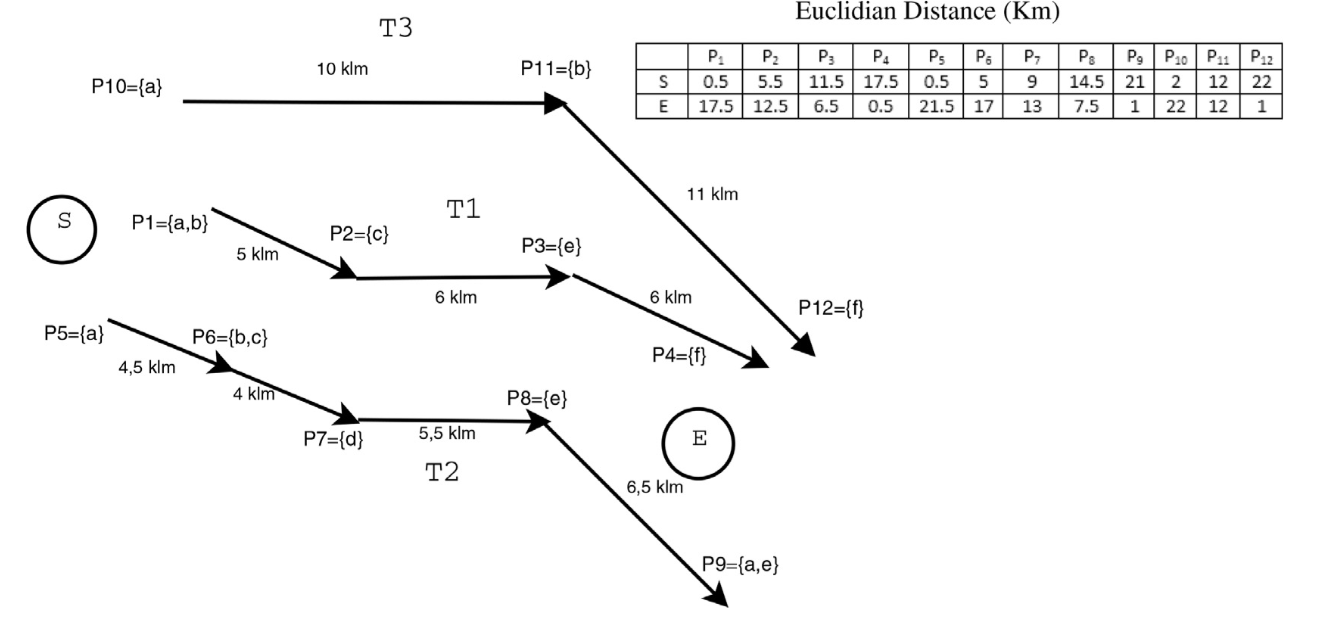
\includegraphics[width=0.75\textwidth]{requirement/query-accuracy.png}
  \bicaption[fig:accuracy]{系统查询结果准确性}{系统查询结果准确性}{Fig}{Accuracy of searching}
\end{figure}

\subsection{系统查询时间特性}
\label{subsec:performance time}
在相似轨迹查询系统中,单机查询点集操作普遍在一秒内完成;若输入点过多或者以一条轨迹作为查询输入,所需的查询时间会到两秒。在交互型系统中,这样这时间操作在可接受范围之内。

\subsection{系统适应性}
\label{subsec:performance flexibility}
相似轨迹查询系统可以根据用户特定的查询需求满足有序或无序、有关轨迹日期、查询数目限制等类型。在满足运行条件的情况可正常运行于各种场景。

\section{本章小结}
\label{sec:requirement conclusion}
系统软件需求分时是在对系统如何开发的概要描述。本章节主要针对相似轨迹查询系统在目前研究环境中,要解决的主要问题进行相似的需求分析,明确系统的问题要求,了解输入与输出,并从用户的角度描述了系统应该具备哪些实际的功能,达到什么的性能标准。与此同时,本章节内容也分析了相似轨迹查询系统在功能性与非功能性中的大致组成框架,为从事相关领域的软件工程师确定用户的基本使用需求。在明确这些需求之后,本文才开始对相似轨迹查询系统进行针对性的设计与构思,为下一章节相似轨迹查询系统的设计与实现提供基础。

%# -*- coding: utf-8-unix -*-
%%==================================================
%% chapter03.tex for SJTU Master Thesis
%% software requirement specification
%%==================================================
%\bibliographystyle{sjtu2}%[此处用于每章都生产参考文献]

\chapter{相似轨迹查询系统设计与实现}
\label{chap:system requirement specification}

\section{本章序言}
\label{sec:introduction}
随着相似轨迹查询这以在科研领域和工业应用中的不断发展,开发相似轨迹查询系统为用户在搜索相似轨迹中提供更方便更可视化的结果。为了明确关于相似轨迹查询系统的设计需求、应用领域与系统功能,在本章节中,本文首先对相似轨迹查询系统的设计与实现作细节说明和具体描述。我们对本章节的目的以及之后说明中会涉及到的名词概念进行解释,以便于之后章节的拓展。该系统是主要以Python进行后端数据处理,系统运行于以Python为基础的Flask Web内部依赖Werkzeurg的工作集服务器。用户只需要通过进行简单操作便可以实现个性化的相似轨迹查询操作,并了解本系统软件的基本工作原理。

\subsection{系统设计编写背景}
\label{subsec:target}
待开发的系统为相似轨迹查询系统。本章节设计概要可作为系统设计人员、系统测试人员、系统使用用户的参考资料与文档。设计实现服务对象为需要进行相似轨迹查询的互联网用户。

\subsection{系统设计编写原则}
\label{subsec:principle}
\begin{itemize}
	\item 准确性:本章节所描述的针对系统的需求,设计系统的功能与行为与目标软件系统产品实现期望相符。
	\item 完整性:包括全部有实际应用意义的系统需求,在功能、性能和设计方面均满足所需的需求。依照<系统软件设计规范说明书>\cite{tuw2002software}的要求,将描述系统需求所需的流程图和名词定义给出完整描述。
	\item 易读性:本章节内容通过简要文字,辅以插图和图标,让读者对象能够清楚了解系统设计中的需求内容。
	\item 可验证性:对于本章节中所编写的系统需求分析与设计内容,读者可通过实际系统进行功能、性能和设计方面上的检查以校对是否与编写内容一致。
\end{itemize}

\subsection{系统名词定义}
\label{subsec:definitions}
表\ref{tab-system definitions}所示。
\begin{table}[!htpb]
  	\centering
		\begin{tabular}{ |p{3cm}||p{9cm}|  }
		\hline
		符号标记 & 符号注释 \\
		\hline
		用户 & 使用相似轨迹查询系统进行轨迹查询人员 \\
		\hline
		管理员 & 相似轨迹查询系统管理员,负责运行权限和控制系统 \\
		\hline
		轨迹数据 & 移动物体上空间上按时间顺序的移动数据记录 \\
		\hline
		GPS & 全球定位系统 \\
		%\hline
		%DESC & 描述 \\
		%\hline
		%DEP & 依赖 \\
		\hline
		\end{tabular}
	\bicaption[tab-system definitions]{相似轨迹查询系统涉及名词定义}{相似轨迹查询系统涉及名词定义}{Table}{A list of definitions and explanations in the system of searching similar trajectories}
\end{table}

\subsection{用户类与特点}
\label{subsec:user characteristics}
相似轨迹查询系统的使用者主要分为轨迹查询用户和管理用户。

对于轨迹查询用户而言,我们通过是否具有在系统中存储这历史轨迹数据分为登录用户和一般用户。一般用户是系统的流动用户,在系统轨迹数据库中不具备历史轨迹。一般用户只能通过向系统输入一组轨迹查询点集以完成相似轨迹查询功能。登录用户可以根据账户信息和密码登录相似轨迹查询系统,使用已有的历史轨迹数据或是自定义的一组轨迹点集实现相似轨迹查询功能。

相似轨迹查询系统中的管理员主要负责登录用户的权限管理和对历史数据的修改处理操作。管理员对于相似轨迹查询系统中违反查询和使用规范的用户可以修改其登录权限以阻止其进一步违规操作。管理员还可以对历史轨迹进行增加、修改和删除操作,以保证系统数据库的实时性和准确性。

\subsection{系统运行环境}
\label{subsec:system environment}

表\ref{tab-system environments}对本系统运行环境进行了描述。
\begin{table}[!htpb]
  	\centering
		\begin{tabular}{ |p{1cm}|p{3.5cm}|p{8.5cm}| }
		\hline
		序号 & 环境需求 & 环境参数 \\
		\hline
		01 & 系统操作系统 & Mac OS 10.11.6  \\
		\hline
		02 & 分布式操作系统 & Ubuntu14.04.1 amd64  \\
		\hline
		03 & 单机PC设备参数 & 处理器 2.6 GHz Intel Core i5且内存大于等于4G\\
		\hline
		04 & 分布式PC设备参数 & 处理器 2.6 GHz Intel Core i5且内存大于等于1G\\
		\hline
		05 & 服务器平台 & Flask0.12/Python2.7.6 \\
		\hline
		\end{tabular}
	\bicaption[tab-system environments]{相似轨迹查询系统运行环境}{相似轨迹查询系统运行环境}{Table}{A list of environment parameters in the system of searching similar trajectories}
\end{table}


\section{系统设计}
\label{sec:overall description}
本文设计的相似轨迹查询系统运行运行于基于Python语言的Flask Web框架,运行过程中需要连接互联网以使用地图接口,系统内部数据为上海私家车数据。系统针对的用户为一般用户和登录用户。一般用户可以目的轨迹点集进行相似轨迹查询,实现路径规划等具体应用,用户在运用过程中需要在地图上点击位置以实现轨迹点击输入;登录用户在一般用户具有功能基础上,用户的历史轨迹在轨迹数据库中有存储,可以实现以一条轨迹为输入的相似轨迹查询,实现拼车或轨迹推荐等具体应用。本系统目前已有依赖于Flask框架和地图接口提供。

\subsection{系统设计分析}
\label{subsec:system build requirement}
将相似轨迹查询系统以Web框架搭建,其最大的好处是给予用户在查询上最大程度的便利。这种便捷主要体现在用户只要连接上互联网,就可以直接通过浏览器访问系统,在线进行相似轨迹的查询。这种网络操作不需要用户在下载系统到终端或者移动端便可以进行实时的相似轨迹查询功能。所以在设计相似轨迹查询这一系统时,主要功能实现均为用户查询而服务,即最重要的一点是完成用户功能部分。

\subsection{系统功能描述}
\label{subsec:product functions}
在相似轨迹查询系统中,一般用户和登录用户都可以使用相似轨迹查询功能。查询结果与用户定义的输入轨迹数据类型(为轨迹点集或一条历史轨迹)、查询的日期、相似轨迹数目阈值和查询是否有序性有关。

在完成登录功能或跳选到直接查询后,用户可以在系统界面中完成查询功任务。相似轨迹查询的主要是通过在地图上以不同颜色和不同粗细的折线端进行表示。在查询结果中,根据与查询输入相似度的相关性,越相似的查询结果轨迹将以越显著的参数表示出来,用户可以一目了然在地图上得出最符合查询的结果的一条或多条轨迹。登录用户可以在地图上点击历史轨迹数据显示系统数据库中存储的某一条与自己相关的历史轨迹。

\subsection{系统设计框架}
\label{subsec:product perspective}
如图\ref{fig:system-architecture}所示相似轨迹查询系统主要由前后端两部分组成。后端部分主要以轨迹预处理、相似轨迹查询和查询请求分析处理为主;前端以部分地图轨迹可视化、查询结果输出、地理位置搜索等部分组成。

\begin{figure}[!htp]
  \centering
  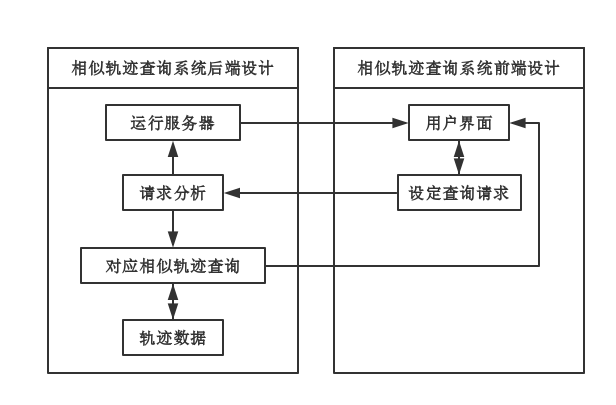
\includegraphics[width=0.8\textwidth]{design/system-architecture.png}
  \bicaption[fig:system-architecture]{相似轨迹查询系统设计框架}{相似轨迹查询系统设计框架}{Fig}{System design architecture}
\end{figure}

针对相似轨迹查询系统的后端处理流程思路主要为,在后台运行服务器代码,接收来自浏览器前端的请求。将请求分析与提前预先设定的资源定位符函数结合,对于数据类型选择是否进行轨迹数据预处理。针对同一的输入轨迹数据点集,进行相似轨迹数据查询功能服务。然后将结果作为请求返回返回给用户。实现一次相似轨迹查询请求过程。与此同时,系统前端主要以实现数据可视化为主,以一个窗口形式将地图数据显示。对于用户感兴趣的地理位置坐标点和历史轨迹数据,可以通过点击地图或历史轨迹数据项目将数据在地图窗口上得以可视化展示。

\subsection{系统处理流程}
图\ref{fig:system-flowchart}展示了相似轨迹查询系统的主要流程。进入相似界面之后,用户可以直接使用系统(即不需要登录)使用系统进行相似轨迹查询,在获取满意的查询结果之后退出系统。同时,如果需要运用登录功能,系统会在登录界面中提醒用户是选择轨迹历史用户登录还是管理员模式登录。对于轨迹历史用户,可以实现相对应的轨迹查询类型并和一般用户一样在得到满意的查询结果之后退出系统。对于管理员而言,他们主要负责对用户权限和轨迹数据处理这一部分工作,在完成管理员工作之后他们也可以按流程退出系统。

\label{subsec:system flow}
\begin{figure}[!htp]
    \centering
    \resizebox{14cm}{!}{
\begin{tikzpicture}[node distance=2cm]

	%\node (input) [startstop] {输入轨迹数据类型判断};
	%\node (input_judge) [decision, below of=input,yshift=-0.5cm,aspect=2.5] {是否为用户指定一组轨迹点集?};
	%\node (ts) [process, right of=input_judge,xshift=5cm] {轨迹简化};
	%\node (iknn) [process, below of=input_judge,yshift=-0.5cm]{增长型k相似轨迹查询};
	%\node (bound_judge) [decision, below of=iknn,yshift=-0.5cm,aspect=2.5]{是否满足相似度上下界条件?};
	%\node (refinement)[process, below of=bound_judge,yshift=-0.5cm]{备选轨迹集筛选};
	%\node (output)[startstop, below of=refinement]{k条最相似轨迹输入};
	

%	\draw [arrow] (input) -- (input_judge);
%	\draw [arrow] (input_judge) -- node[anchor=south]{否}(ts);
%	\draw [arrow] (input_judge) -- node[anchor=west]{是}(iknn);
%	\draw [arrow] (ts) |- (iknn);
%	\draw [arrow] (iknn) -- (bound_judge);
%	\draw [arrow] (bound_judge.west) |- node[anchor=south]{否}(iknn.west);
%	\draw [arrow] (bound_judge.south) -- node[anchor=west]{是}(refinement.north);
%	\draw [arrow] (refinement) -- (output);

	\node (begin) [startstop,font=\bf,fill=green!20] {进入系统界面};
	\node (login_judge) [decision, below of=begin, yshift=-0.5cm, aspect=2.5]{是否需要登录};
	\node (general) [process, right of=login_judge, xshift=3cm]{一般用户};
	\node (login_type_judge) [decision, below of=login_judge, yshift=-0.5cm, aspect=2.5]{是否为管理员};
	\node (history) [process, right of=login_type_judge, xshift=3cm]{登录用户};
	\node (admin) [process, below of=login_type_judge]{管理员操作};
	\node (search) [process, right of=history, xshift=3cm]{相似轨迹查询};
	\node (is_search_good) [decision, below of=search, aspect=2.5]{是否满意查询结果};
	\node (does_admin_finish) [decision, below of=admin, aspect=2.5]{管理员操作是否完成};
	\node (finish) [process, below of=history]{系统处理完成};
	\node (stop) [startstop, below of=finish,font=\bf,fill=green!20]{退出系统界面};
	
	
	
	\draw [arrow](begin.south) -- (login_judge.north);
	\draw [arrow](begin.east) -| node[anchor=south]{直接查询模式}(general.north);
	\draw [arrow](login_judge.east) -- node[anchor=north]{否}(general.west);
	\draw [arrow](login_judge.south) -- node[anchor=west]{是}(login_type_judge.north);
	\draw [arrow](login_type_judge.east) -- node[anchor=north]{否}(history.west);
	\draw [arrow](login_type_judge.south) -- node[anchor=west]{是}(admin.north);
	\draw [arrow](general.east) -| (search.north);
	\draw [arrow](history.east) -- (search.west);
	
	\draw [arrow](search.south) -- (is_search_good.north);
	\draw [arrow](is_search_good.east) |- node[anchor=west]{否}(search.east);
	\draw [arrow](is_search_good.west) -- node[anchor=north]{是}(finish.east);
	
	\draw [arrow](admin.south) -- (does_admin_finish.north);
	\draw [arrow](does_admin_finish.west) |- node[anchor=east]{否}(admin.west);
	\draw [arrow](does_admin_finish.east) |- node[anchor=east]{是}(finish.west);
	
	\draw [arrow](finish.south) -- (stop.north);

\end{tikzpicture}

}
    \bicaption[fig:system-flowchart]{相似轨迹查询系统处理流程图}{相相似轨迹查询系统处理流程图}{Fig}{A flow chart of searching similar trajectory system}
\end{figure}

%%%%%%%%%%%

\section{接口设计}
\label{sec:interface design}

\subsection{外部接口}
\label{subsec:external interface}
由于相似轨迹查询系统没有直接的硬件系统设计,该系统中没有直接的外部硬件接口。存储于系统中的GPS轨迹数据由系统内部文件系统或数据库来管理,其中的服务器或数据的连接操作由设备内部的操作系统负责。运行环境中对系统所需要运行的硬件设备和操作系统环境在表\ref{tab-system environments}予以表述。

\subsection{内部接口}
\label{subsec:internal interface}
相似轨迹查询系统内部数据传递主要由三层结构实现
\begin{itemize}
	\item 系统表达层
	\item 系统逻辑层
	\item 系统数据层
\end{itemize}
系统表达层使用flask提供的Jinja2\cite{flasklibrary}模板实现系统的可视化界面和网页交互界面,采用基于Bootstrap的设计框架进行直接表达;逻辑层采用Python中的修饰符和flask中的将请求与数据处理结合;数据层通过直接对分布式文件系统读写或sqlite3数据库连接进行数据处理。

\begin{figure}[!htp]
    \centering
    \resizebox{!}{!}{
\begin{tikzpicture}[node distance=2cm]

	\node (top) [process] {系统表示层};
	\node (mid) [process, below of=top] {系统逻辑层};
	\node (bottom) [process, below of=mid] {系统数据层};
	
	\draw [arrow] (top.south) -- (mid.north);
	\draw [arrow] (mid.north) -- (top.south);
	\draw [arrow] (mid.south) -- (bottom.north);
	\draw [arrow] (bottom.north) -- (mid.south);
\end{tikzpicture}

}
    \bicaption[fig:systemlevel]{相似轨迹查询系统数据层次}{相似轨迹查询系统数据层次}{Fig}{Data passing level in the system}
\end{figure}

为了满足上述三层结构的正常实现,我们设计的内部接口主要为以下几种。表达层与逻辑层本文实现系统采用值传递的接口方式。表达层获取逻辑层传递的值进行界面刷新处理,同时逻辑层接收表达层的请求值以进行后续处理。逻辑层与数据层之间使用文件系统或数据库已有的命令操作,逻辑层借用底层提供的接口实现对数据的处理操作,数据层对逻辑层提供数据查询支持。

\subsection{用户接口}
\label{ubsection:user interface}
用户必须具有支持地图加载功能浏览器,本文测试系统所使用的浏览器为\emph{Safari9.2.1}。相似轨迹查询系统主要通过用户Web页面界面进行实时的信息交互与查询处理,达到信息传递和查询结果可视化的目的。该系统主要提供以下几种用户接口:
\begin{itemize}
	\item 用户登录与注销接口
	\item 功能选择接口
	\item 地理位置点查询接口
	\item 相似轨迹查询接口
	\item 历史轨迹展示接口
\end{itemize}

%%%%%%%%%%%

\section{系统总体结构}
\label{sec:system analysis}
根据系统处理流程:
\begin{itemize}
	\item 系统初始时,进入系统主界面。可以完成一般操作或选择登录实现历史轨迹操作。
	\item 如果用户登录成功,则会显示用户信息和对应的历史轨迹以完成用户需求工作。
	\item 当用户完成查询工作,可以选择注销退出用户界面或直接选择关闭浏览器以退出系统。
\end{itemize}

我们大致按照下述章节来对系统进行总体结构设计。

\subsection{系统组成模块}
\label{subsec:component analysis}
\begin{figure}[!htp]
    \centering
    \resizebox{!}{!}{\begin{tikzpicture}[
      every node/.style = {draw, rounded corners=3pt, semithick},
            ROOT/.style = {inner sep=3mm, fill=red!20, font=\bfseries},
              L1/.style = {fill=blue!30},
              L2/.style = {fill=green!20},
              L3/.style = {fill=green!1, grow=down, xshift=1em, anchor=west, 
      edge from parent path={(\tikzparentnode.south) |- (\tikzchildnode.west)}},
edge from parent/.style = {draw, thick},
              LD/.style = {level distance=#1ex},
             LD1/.style = {level distance=6ex},
             LD2/.style = {level distance=12ex},
             LD3/.style = {level distance=18ex},
         level 1/.style = {sibling distance=50mm}
                        ]
    % Parents
\node[ROOT] {相似轨迹查询系统}
    [edge from parent fork down]
    child{node[L2] {用户模块}
      child[L3,LD1]   {node[L3]   {用户登录模块}}
      child[L3,LD2]   {node[L3]   {轨迹查询模块}}
      child[L3,LD3]   {node[L3]   {地理查询模块}}
      }
    child{node[L2] {管理员模块}
      child[L3,LD1]  {node[L3]   {用户管理模块}}
      child[L3,LD2]  {node[L3]   {轨迹管理模块}}
      };
\end{tikzpicture}}
    %\begin{tikzpicture}[
      every node/.style = {draw, rounded corners=3pt, semithick},
            ROOT/.style = {inner sep=3mm, fill=red!20, font=\bfseries},
              L1/.style = {fill=blue!30},
              L2/.style = {fill=green!20},
              L3/.style = {fill=green!1, grow=down, xshift=1em, anchor=west, 
      edge from parent path={(\tikzparentnode.south) |- (\tikzchildnode.west)}},
edge from parent/.style = {draw, thick},
              LD/.style = {level distance=#1ex},
             LD1/.style = {level distance=6ex},
             LD2/.style = {level distance=12ex},
             LD3/.style = {level distance=18ex},
         level 1/.style = {sibling distance=50mm}
                        ]
    % Parents
\node[ROOT] {相似轨迹查询系统}
    [edge from parent fork down]
    child{node[L2] {用户模块}
      child[L3,LD1]   {node[L3]   {用户登录模块}}
      child[L3,LD2]   {node[L3]   {轨迹查询模块}}
      child[L3,LD3]   {node[L3]   {地理查询模块}}
      }
    child{node[L2] {管理员模块}
      child[L3,LD1]  {node[L3]   {用户管理模块}}
      child[L3,LD2]  {node[L3]   {轨迹管理模块}}
      };
\end{tikzpicture}
    \bicaption[fig:module]{相似轨迹查询系统模块组成}{相似轨迹查询系统模块组成}{Fig}{Modules of Searching similar trajectories system}
\end{figure}

如图\ref{fig:module}所示,本文相似轨迹查询模块主要由以下两个部分组成:
\begin{enumerate}
	\item 用户模块
	\begin{itemize}
		\item 用户登录模块:完成用户登录功能,用户通过在轨迹数据中的id号码和密码进行密钥登录
		\item 轨迹查询模块:完成用户相似轨迹查询功能,可以将相似轨迹查询结果展示在地图上。
		\item 地理查询模块:完成用户对地理位置点的查询,用户在不知道地理点具体位置时候可以通过这一查询功能完成对地理位置在地图上的定位。
	\end{itemize}
	\item 管理员模块
	\begin{itemize}
		\item 用户管理模块:完成管理员对登录用户的权限管理和信息管理。
		\item 轨迹管理模块:完成管理员对系统内部轨迹数据的增删改除功能。
	\end{itemize}
\end{enumerate}

\subsection{系统功能模块详细设计}
\label{subsec:system module details description}

\begin{enumerate}
	\item \textbf{用户登录模块}
	\begin{itemize}
		\item 模块编号:M1
		\item 模块名称:用户登录模块
		\item 模块输入:用户名信息与对应密码
		\item 模块处理:决定用户信息与对应密码是否匹配
		\item 模块输出:若匹配则跳转到功能页面,否则重新输入
	\end{itemize}
	
	\item \textbf{轨迹查询模块}
	\begin{itemize}
		\item 模块编号:M2
		\item 模块名称:轨迹查询模块
		\item 模块输入:查询轨迹点集或历史轨迹
		\item 模块处理:根据输入进行相似轨迹查询
		\item 模块输出:在地图上输出k条最相似轨迹查询结果
	\end{itemize}
	
	\item \textbf{地理查询模块}
	\begin{itemize}
		\item 模块编号:M3
		\item 模块名称:地理查询模块
		\item 模块输入:查询地理点名称信息
		\item 模块处理:调用地图查询接口寻找对应定理信息的坐标
		\item 模块输出:在地图上显示具体位置并在界面中显示地理点坐标
	\end{itemize}
	
	\item \textbf{用户管理模块}
	\begin{itemize}
		\item 模块编号:M4
		\item 模块名称:用户管理模块
		\item 模块输入:用户信息和对应操作
		\item 模块处理:管理员对相应用户进行权限限制操作
		\item 模块输出:被限制用户暂时无法使用系统
	\end{itemize}
	
	\item \textbf{轨迹管理模块}
	\begin{itemize}
		\item 模块编号:M5
		\item 模块名称:轨迹管理模块
		\item 模块输入:轨迹信息
		\item 模块处理:管理员根据输入的轨迹信息对轨迹数据库进行更新操作
		\item 模块输出:更新后的系统轨迹数据库
	\end{itemize}
\end{enumerate}

%\begin{figure}[!htp]
%  \centering
%  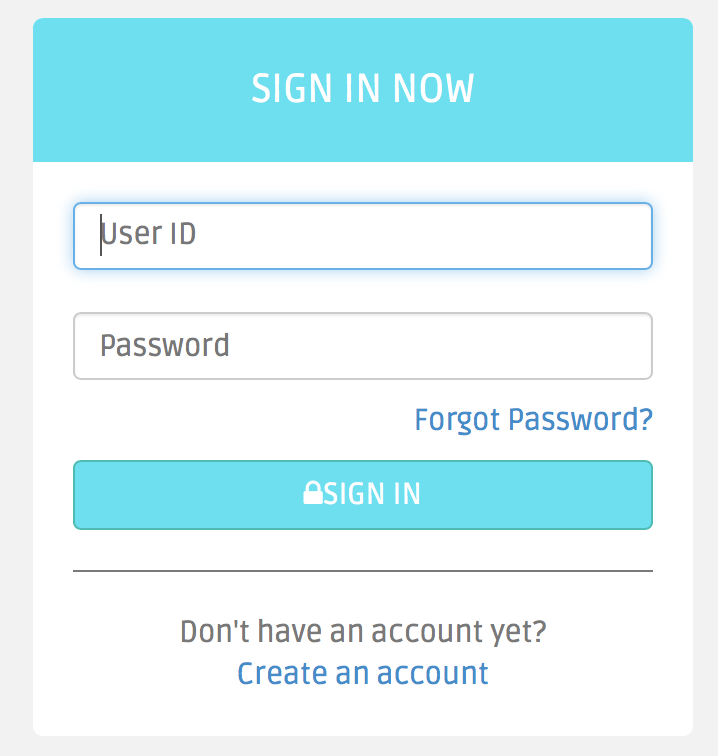
\includegraphics[width=0.4\textwidth]{design/login.png}
  %\hspace{0.5cm}
  %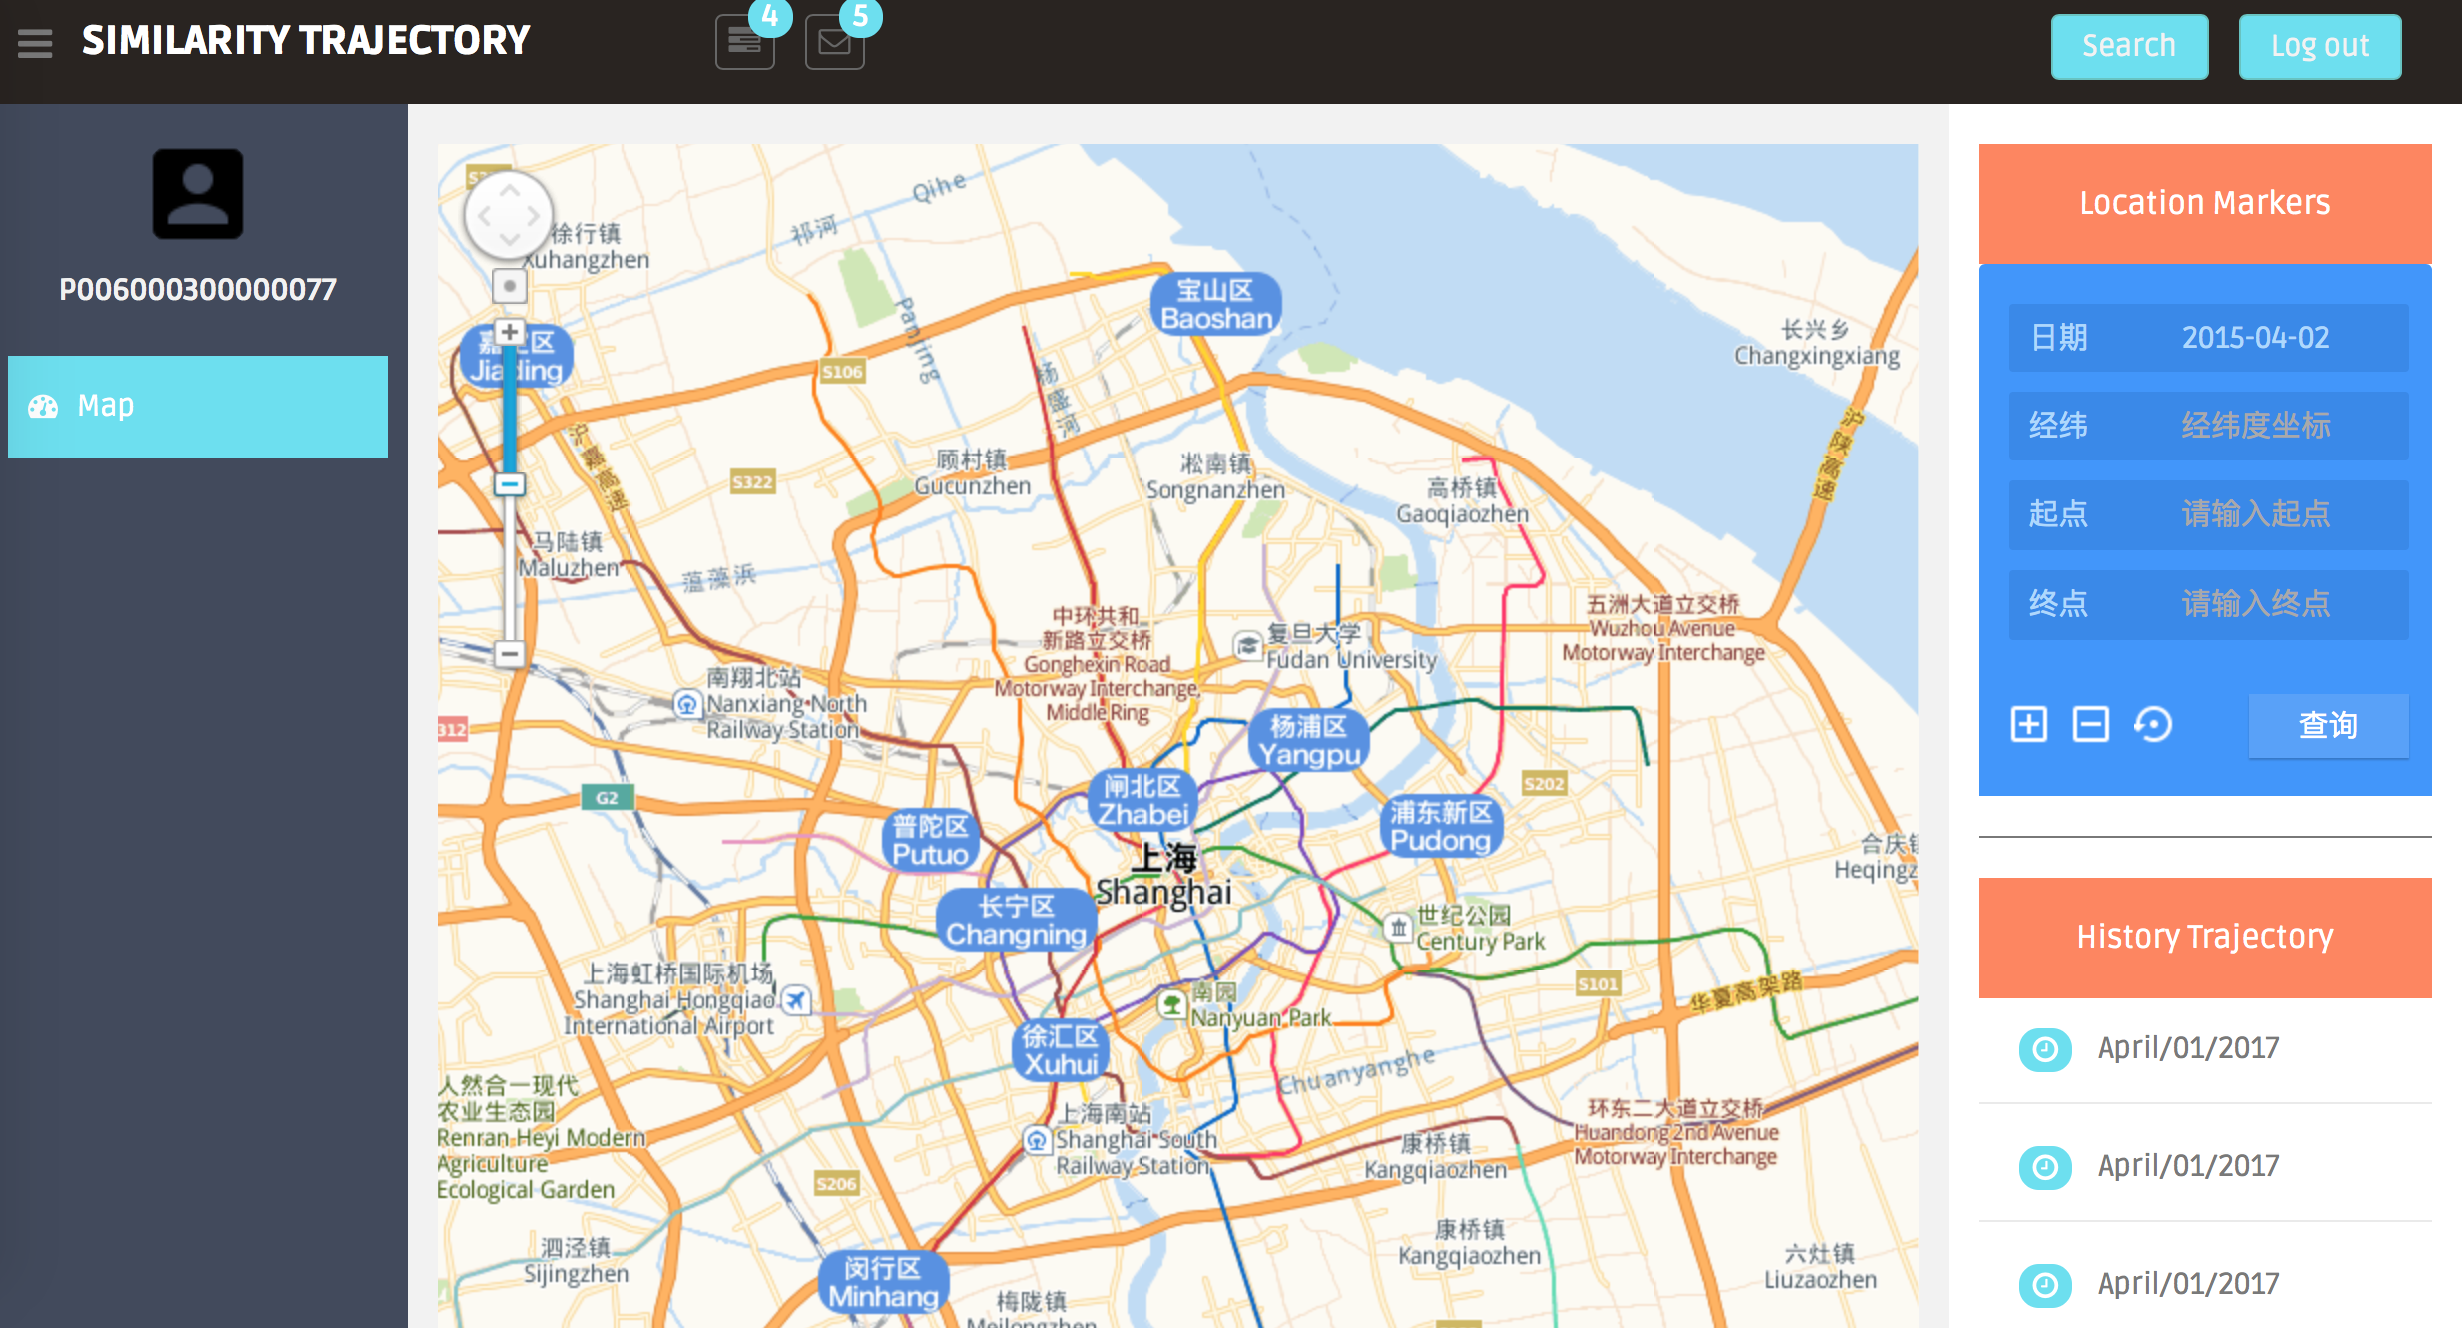
\includegraphics[width=0.6\textwidth]{design/interface.png}
%  \bicaption[fig:login-interface]{用户登录界面}{用户登录界面}{Fig}{User login interface design}
%\end{figure}


\section{系统用户界面设计}
\label{sec:window interface}

图\ref{fig:user-interface}和图\ref{fig:map-interface}分别为用户使用功能的窗口和用户使用系统功能的主要界面设计实现截图。

\begin{figure}[!htp]
	\centering
	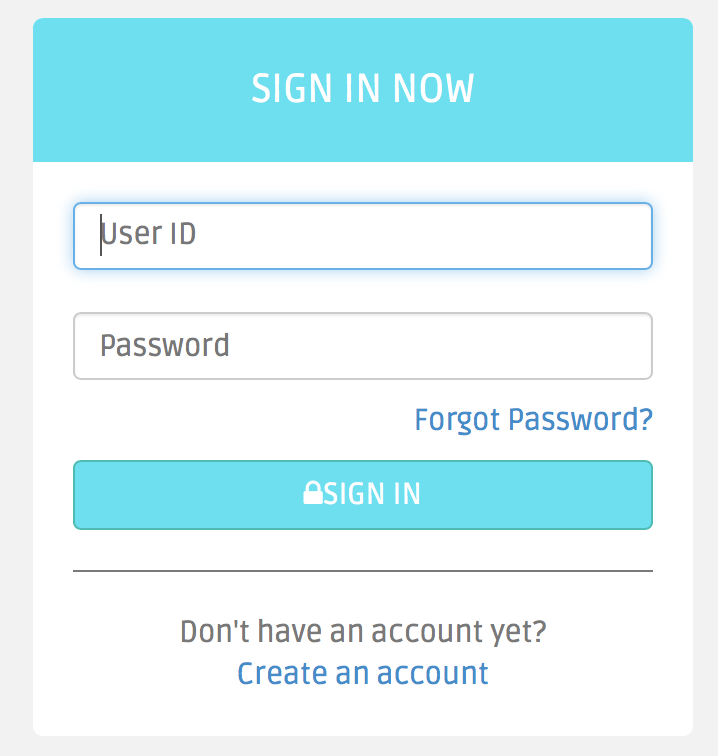
\includegraphics[width=0.3\textwidth]{design/login.png}
	\hspace{0.3cm}
	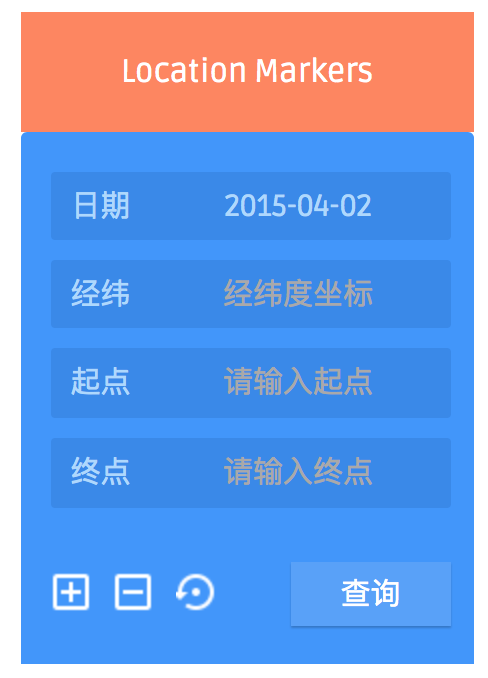
\includegraphics[width=0.3\textwidth]{design/search.png}
   	\hspace{0.3cm}
   	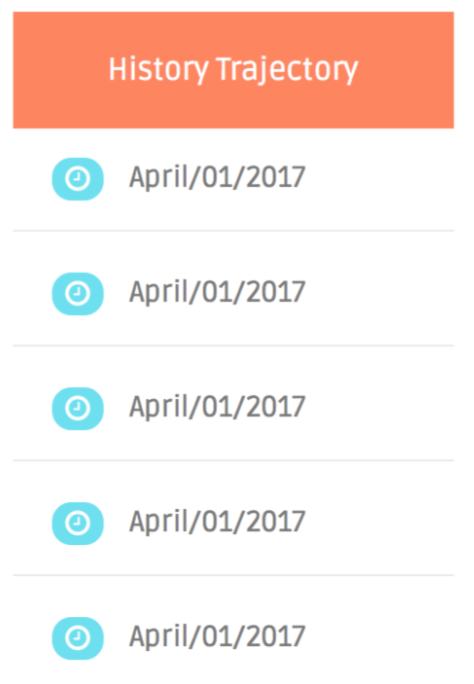
\includegraphics[width=0.3\textwidth]{design/history-trajectory.png}
   	\bicaption[fig:user-interface]{用户功能窗口}{用户功能窗口}{Fig}{User function window interface}
\end{figure}

\begin{figure}[!htp]
  \centering
  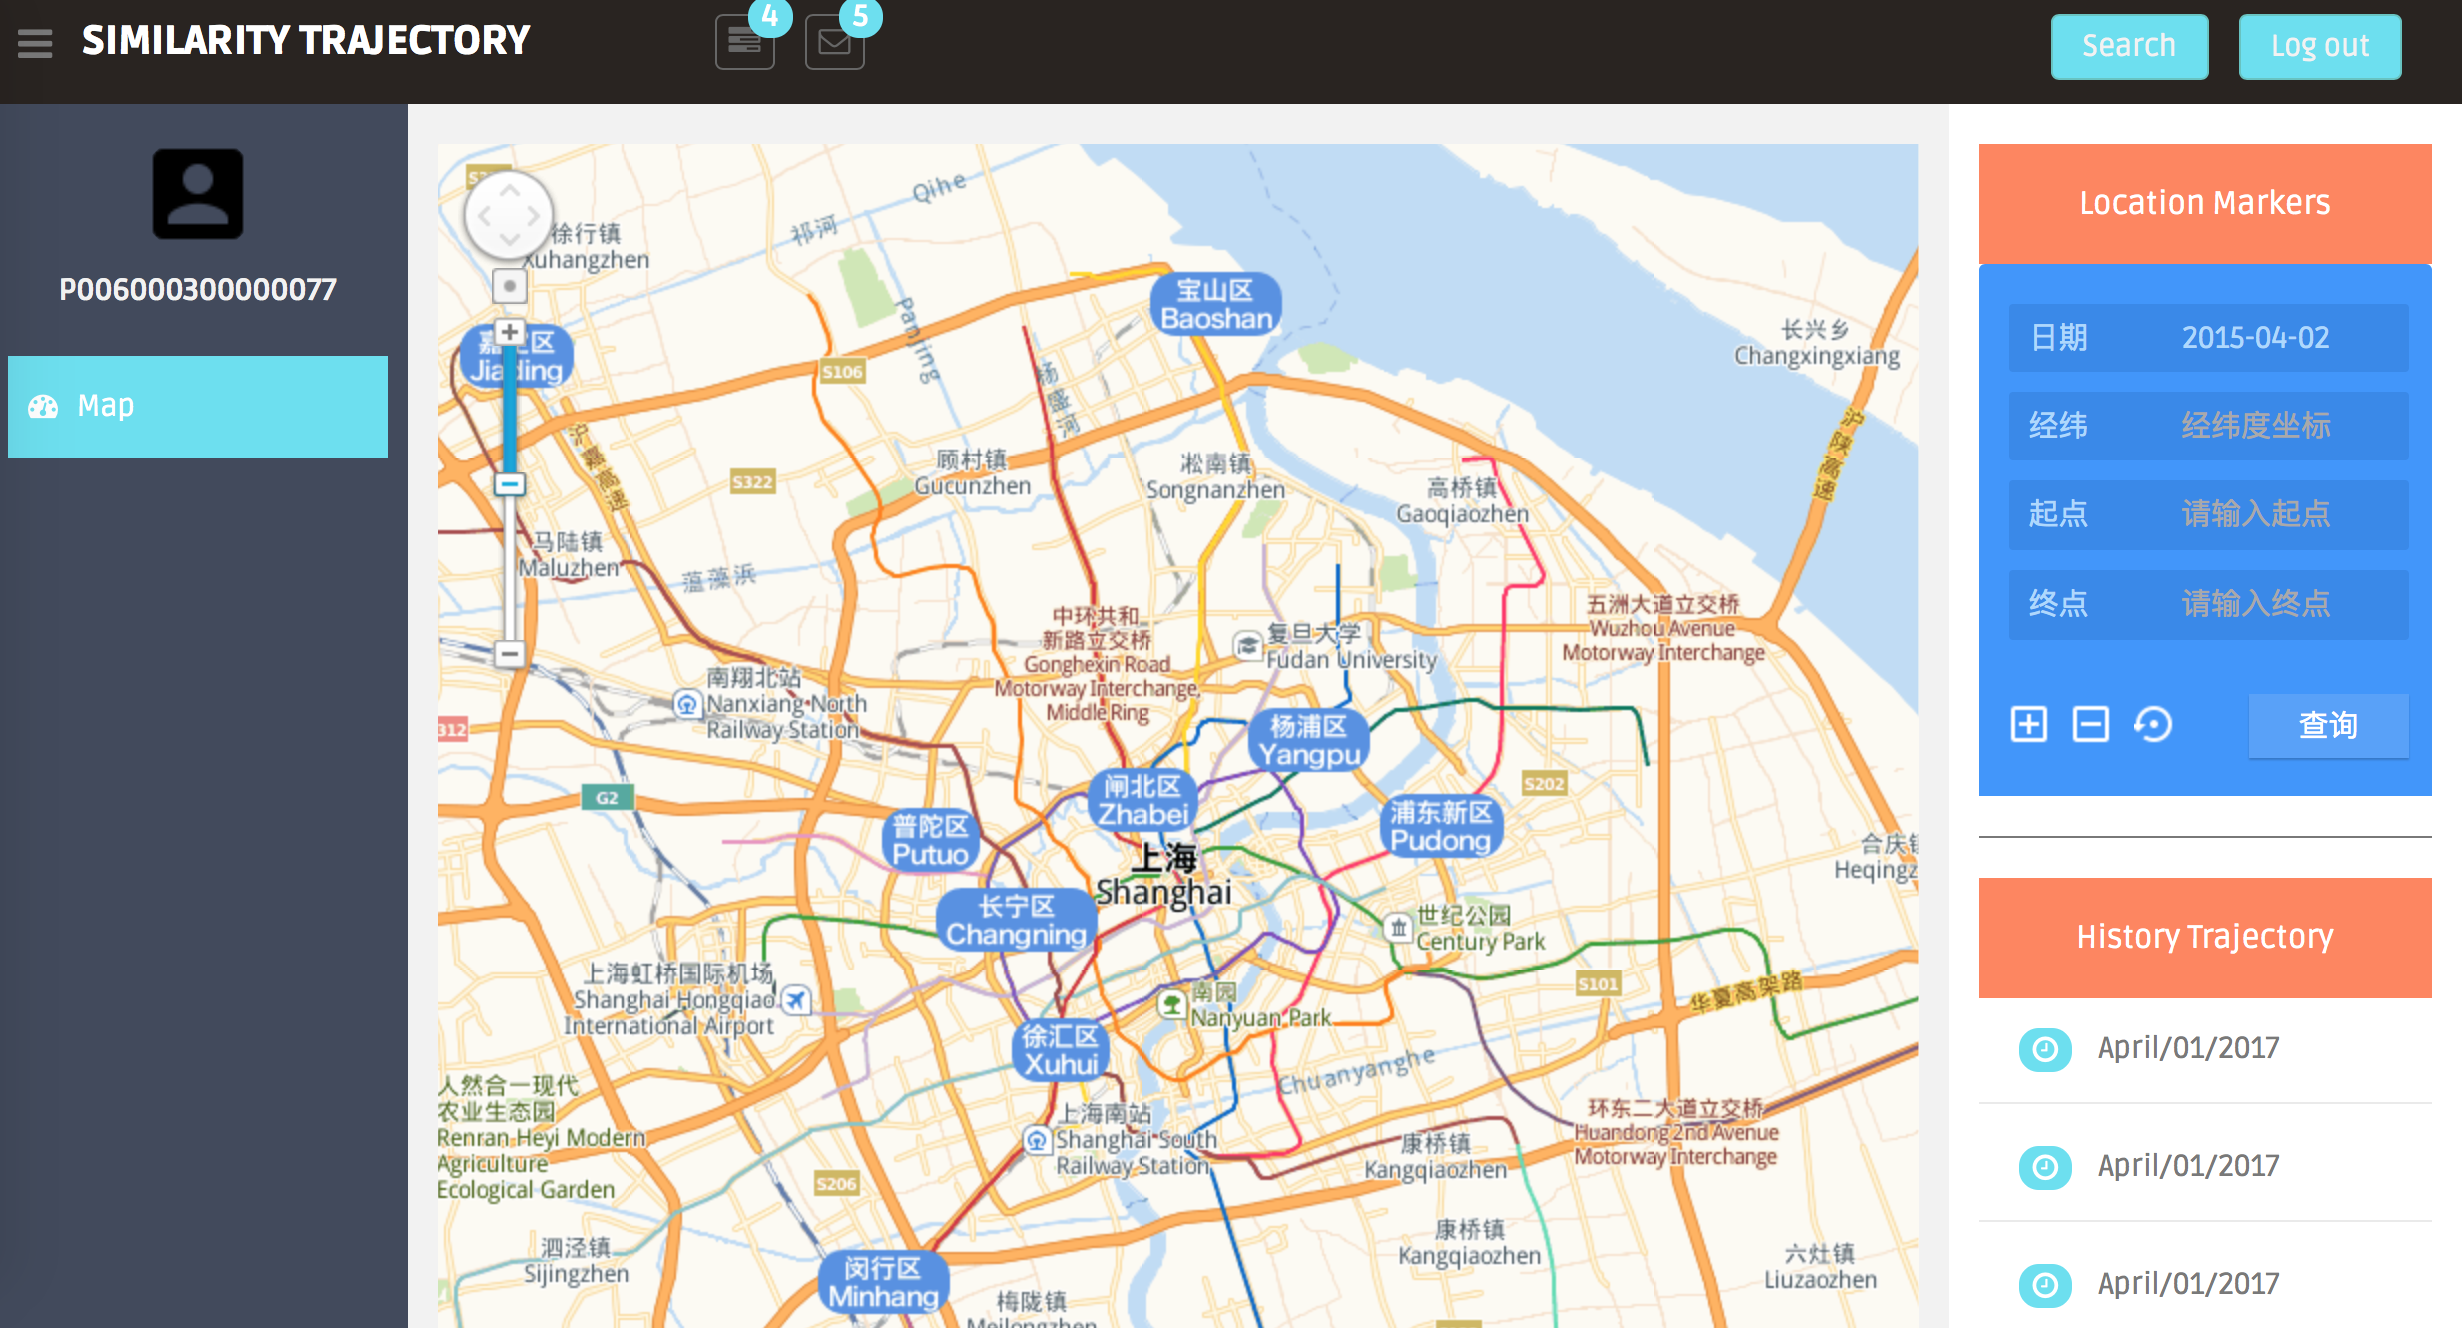
\includegraphics[width=0.7\textwidth]{design/interface.png}
  \bicaption[fig:map-interface]{用户地图界面设计}{用户地图界面设计}{Fig}{User interface design}
\end{figure}

%\begin{figure}[!htp]
%  \centering
%  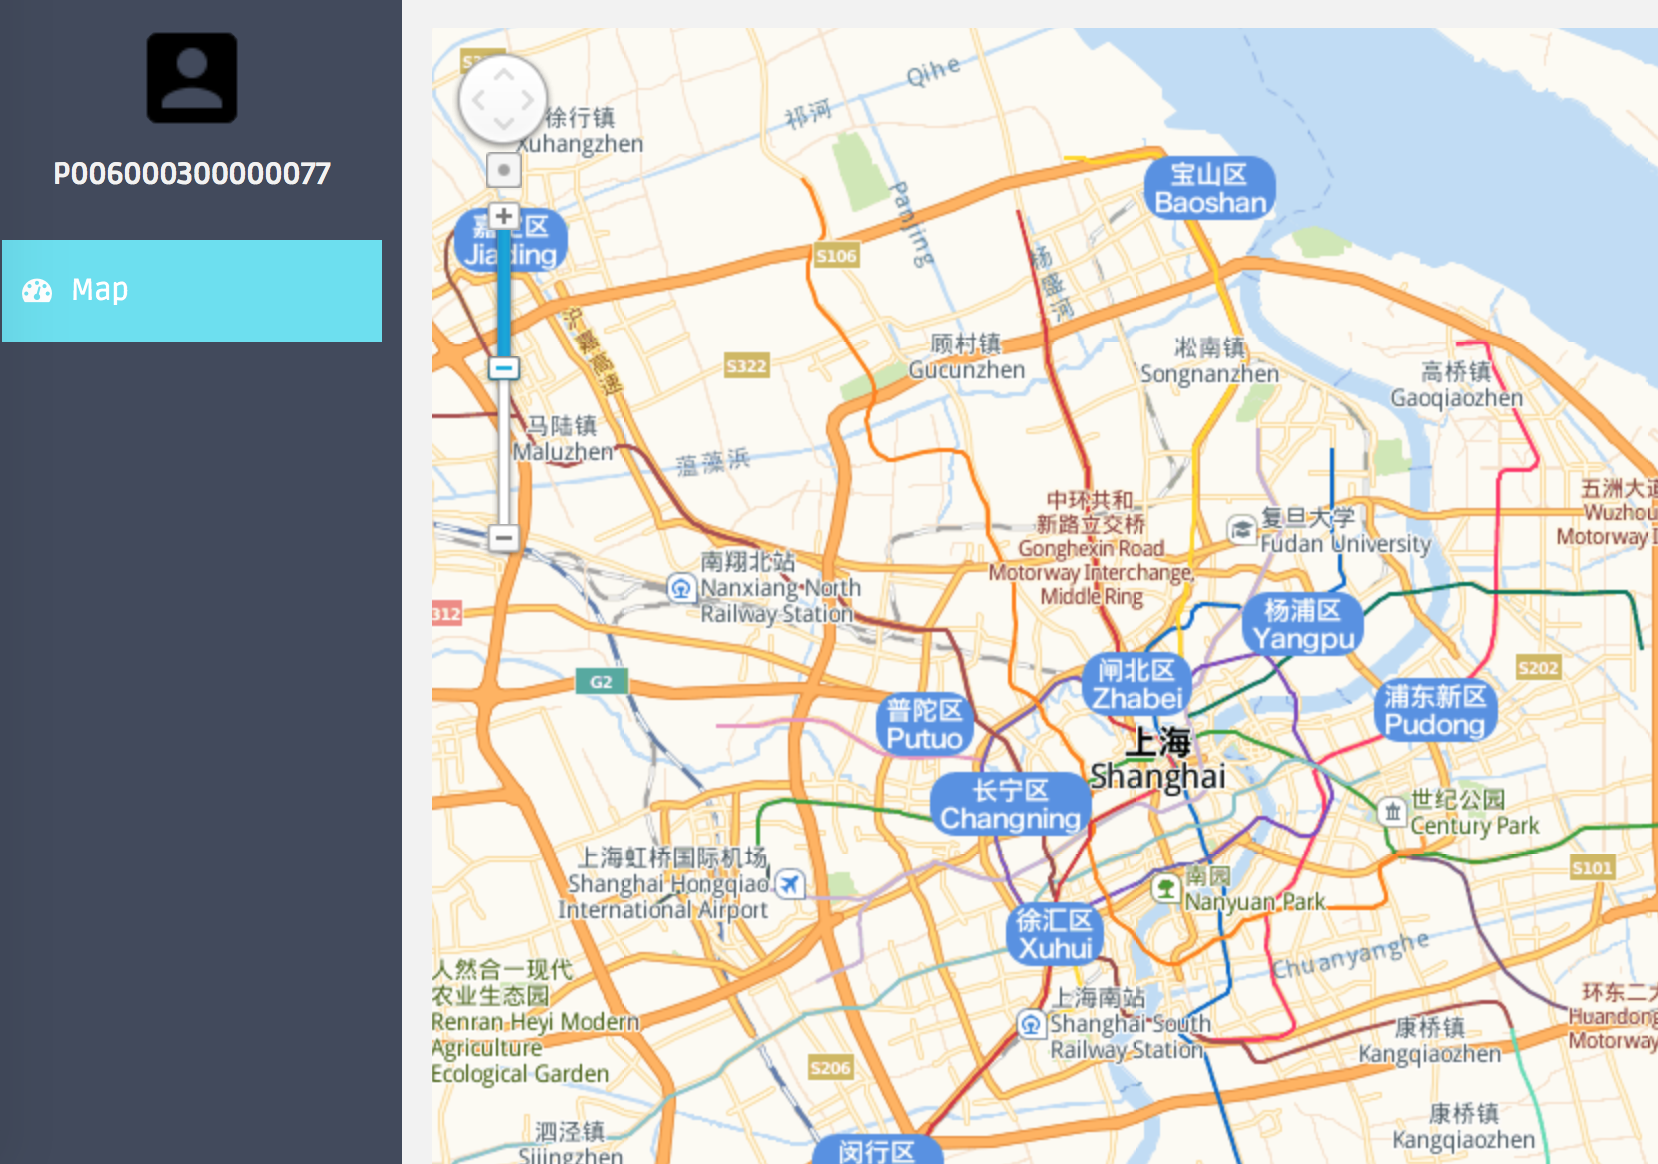
\includegraphics[width=0.4\textwidth]{design/map.png}
%  \bicaption[fig:function-interface]{用户地图界面设计}{用户地图界面设计}{Fig}{User map function interface design}
%\end{figure}


%\subsection{系统性能分析}
%\label{subsec:performance analysis}
%(系统运行截图和系统性能表格)

\section{本章小结}
\label{sec:design conclusion}
本章基于系统需求分析,将上一章节中对系统的需求描述展转换成具体接口设计结构与对应模块设计结构:将一个复杂的相似轨迹查询系统以小模块子系统的结构进行分解,并建立模块之间的数据传递和功能调用关系,确定对应接口对应的数据传递层。在这里,对相似轨迹查询系统进行设计阐述的主要目的是将需求逻辑转化为功能模块实现,以便开发人员在开发这一系统时能清晰明了明确自己负责的模块开发部分,也便于用于理解系统的运行逻辑情况。

%# -*- coding: utf-8-unix -*-
%%==================================================
%% test and evaluation
%%==================================================

%\bibliographystyle{sjtu2}%[此处用于每章都生产参考文献]

\chapter{系统测试与评价}
\label{chap:evaluation}
在系统软件开发中,系统测试与评价是本文关注的重点:系统的开发是否具备完整的基础功能、系统查询过程中能稳定在什么层次的性能水平,以及系统是否有足够的缺陷应对措施都是我们所需要关注的问题。

本章节主要给出系统测试文档。依据前面章节所提出的系统需求分析和系统设计实现文档,对现阶段开发的系统进行功能与性能在综合测试与评价。在测试过程中我们是主要依赖于测试原理和测试手段:测试原理主要根据系统测试理论指导,测试手段是运行系统进行实际应用查询以获取测试数据。另一方面,我们在测试过程中尽可能地模拟实际应用过程,以从用户的角度去测试系统是否具备实用性,因此系统运行环境中我们使用的数据集以实际轨迹数据为主。

\section{引言}
\label{sec:evaluation introduction}

\subsection{编写目的}
\label{subsec:purpose}
编写本章节测试与评价文档主要有以下几个目的:
\begin{itemize}
	\item 验证系统内部算法实现的正确性与可行性。
	\item 对系统产品的质量进行评价。通过对系统测试结果的数据分析以评估所设计实现的系统是否符合预期使用价值。
	\item 分析测试过程中使用的数据和信息,为之后的产品拓展提供参考资料。
	\item 分析系统产品目前阶段所存在的性能不足和使用缺陷,为下一阶段工作的提高做准备。
\end{itemize}

\subsection{针对用户}
\label{subsec:people}
\begin{itemize}
	\item 相似轨迹查询系统开发人员
	\item 相似轨迹查询系统管理人员
	\item 相似轨迹查询系统使用用户
\end{itemize}

\subsection{缺陷定义}
\label{subsec:software flaw definition}
\begin{itemize}
	\item 软件系统未实现需求分析和系统设计中的功能
	\item 软件系统未满足用户或客户的期望与需求
	\item 软件系统未满足在需求分析中预计的功能准确性与完备性。
	\item 软件测试人员难以理解系统设计而无法测试
	\item 用户个体对系统使用过程后认为系统体验不佳、系统查询效果不良。
\end{itemize}

\subsection{测试环境数据}
\label{subsec:environment}

\subsubsection{测试数据集}
\label{subsubsec:dataset}
上海私家车OBD轨迹数据集\cite{NRL}。其中有三种数据格式的数据。在系统测试中,我们选择数据定义为GPS\_routine\_3的第三种数据类型私家车轨迹数据,如表\ref{tab-gpsroutine3}所示:
	\begin{table}[!htpb]
  	\centering
		\begin{tabular}{ |p{2cm}|p{3.5cm}|p{2cm}|p{4.5cm}| }
		\hline
		字段名称 & 含义 & 类型 & 备注\\
		\hline
		id & 记录号 & & 自增id \\
		\hline
		obd\_id & obd设备号 & String & \\
		\hline
		经纬度 & 地理坐标 &  & \\
		\hline
		obd端时间 & & 时间 & yyyy-mm-dd 时分秒\\
		\hline
		车辆状态 & 速度、发动机转速 & & \\
		\hline 
		\end{tabular}
		\bicaption[tab-gpsroutine3]{系统测试选取轨迹数据格式}{系统测试选取轨迹数据格式}{Table}{A list of data fields of private trajectory data}
	\end{table}
	
	本文选择其中时间范围为2015年4月份的轨迹数据。原始轨迹数据的一条数据包含表\ref{tab-gpsroutine3}的中所有的字段值,其中数据项目以时间顺序依次存储。系统处理过程中,假设在第三种数据结构下,如果一个obd用户的两个坐标点时间间隔超过半个小时,则两个坐标点属于不同的两天轨迹数据。基于这一假设,系统在预处理阶段轨将每个用户的轨迹点划分到对应的轨迹数据中,生成用户的轨迹历史数据。
	
\begin{figure}[!htp]
  \centering
  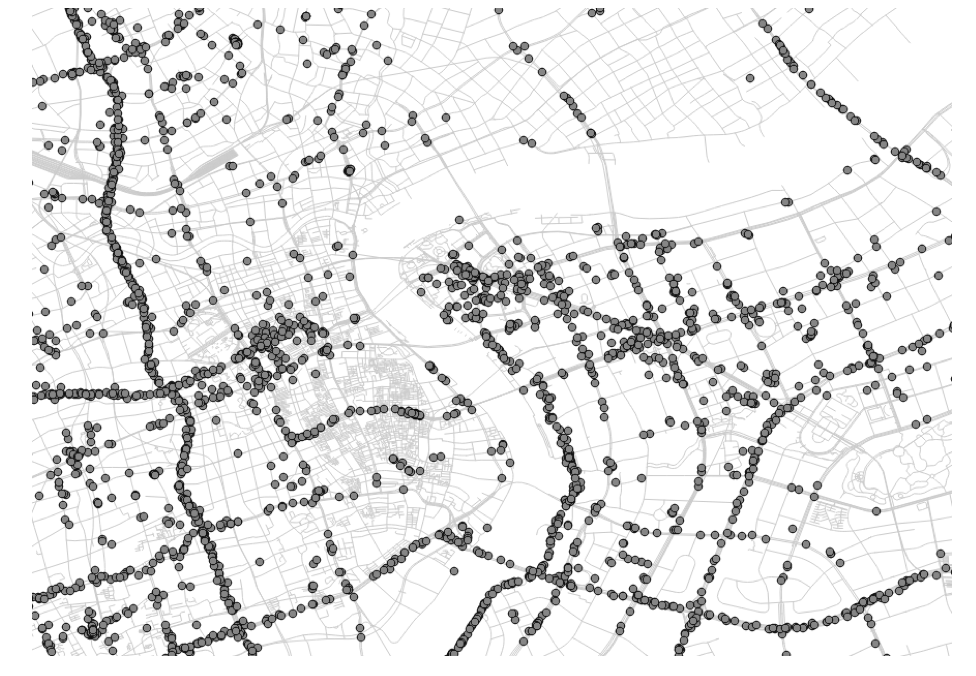
\includegraphics[width=0.5\textwidth]{evaluation/obd.png}
  \bicaption[fig:obd data]{上海市私家车轨迹数据样例}{上海市私家车轨迹数据样例\cite{NRL}}{Fig}{An example of Shanghai OBD private trajectories data}
\end{figure}


\subsubsection{测试设备环境}
\label{subsubsec:device}
\begin{enumerate}
	\item 单机测试环境
	\begin{itemize}
		\item Mac OS X EI Caption操作系统
		\item 2.6 GHz Intel Core i5处理器
		\item 8GB 1600 MHz DDR3内存
	\end{itemize}
	\item 分布式集群处理环境
	\begin{itemize}
		\item Ubuntu14.04 amd64操作系统
		\item 2.6 GHz Intel Core i5处理器
		\item 1GB DDR3内存
	\end{itemize}
\end{enumerate}

\section{系统测试概要}
\label{sec:general description}
本章节大体从系统的功能和性能两个方面入手对本文所设计并实现的相似轨迹查询系统进行测试。在功能测试方面,测试主要的目的在于考察系统实现是否完成需求分析与系统设计中的预期功能,保证用户在使用系统过程中能够正常使用任一一个系统的子功能从而保证用户使用系统的流畅性与完整性;在性能测试方面,测试主要的目的在于分析系统实现是否能够高效并准确地为用户提供查询结果或是其他交互方面为用户提供良好的使用体验,在网页系统中,良好的交互性与结果的准确性是一个系统在用户群中不断使用的根本保证。

\section{系统测试描述}
\label{sec:function test}

\subsection{功能测试描述}
\label{subsec:function test description}
本文所设计的功能测试中的各类操作主要针对组成相似轨迹查询系统的的单一功能模块,每个操作步骤对应的就是一个功能点,即功能模块。由于本文所设计的相似轨迹查询系统由用户模块和管理员模块两个大部分组成,因此我们需要再分别对两个主要模块内部的功能模块进行系统使用测试。

\subsection{性能测试描述}
\label{subsec:performance test description}
在单机测试环境中,本文所设计的性能测试主要是位了获取系统在各种应用或者不同输入参数的情况下对查询效率和查询准确的反应情况。由于该系统的主要针对群里是用户对象,因此性能是本次测试中的重点考虑因素,一个良好的系统应该能够给予用户较好的交互体验。由于系统设计与实现并不一定合理,本文尽可能的考虑系统在查询过程中的上限性能,找出在现阶段中系统可能仍然存在的不足或亟待改善的部分,为今后系统的拓展和升级提供参考思路。

对于分布式性能的测试,由于系统设备限制问题,本文在本次测试中仅给出在分布式环境在系统完成任务时所需要的查询时间。我们在测试中证明对于分布式,在对于目前查询性能影响较大的时间因子在于读取HDFS文件系统中。也将相似轨迹查询在分布式集群处理环境下的性能提高目标放在今后系统能够运行在更优秀的集群环境中。

\section{系统测评结果}
\label{sec:test result}

\subsection{功能测试结果}
\label{subsec:function test result}

\subsection{性能测试结果}
\label{subsec:performance test result}

在性能测试方面,对于单机测试本文设定一下测试条件
\begin{itemize}
	\item 测试变量:相似轨迹查询数目和查询位置点数目。
	\item 测试指标:相似轨迹查询时间和查询准确度。
	\item 测试类型:相似轨迹无序查询和有序查询。
\end{itemize}

\begin{figure}[!htp]
  \centering
  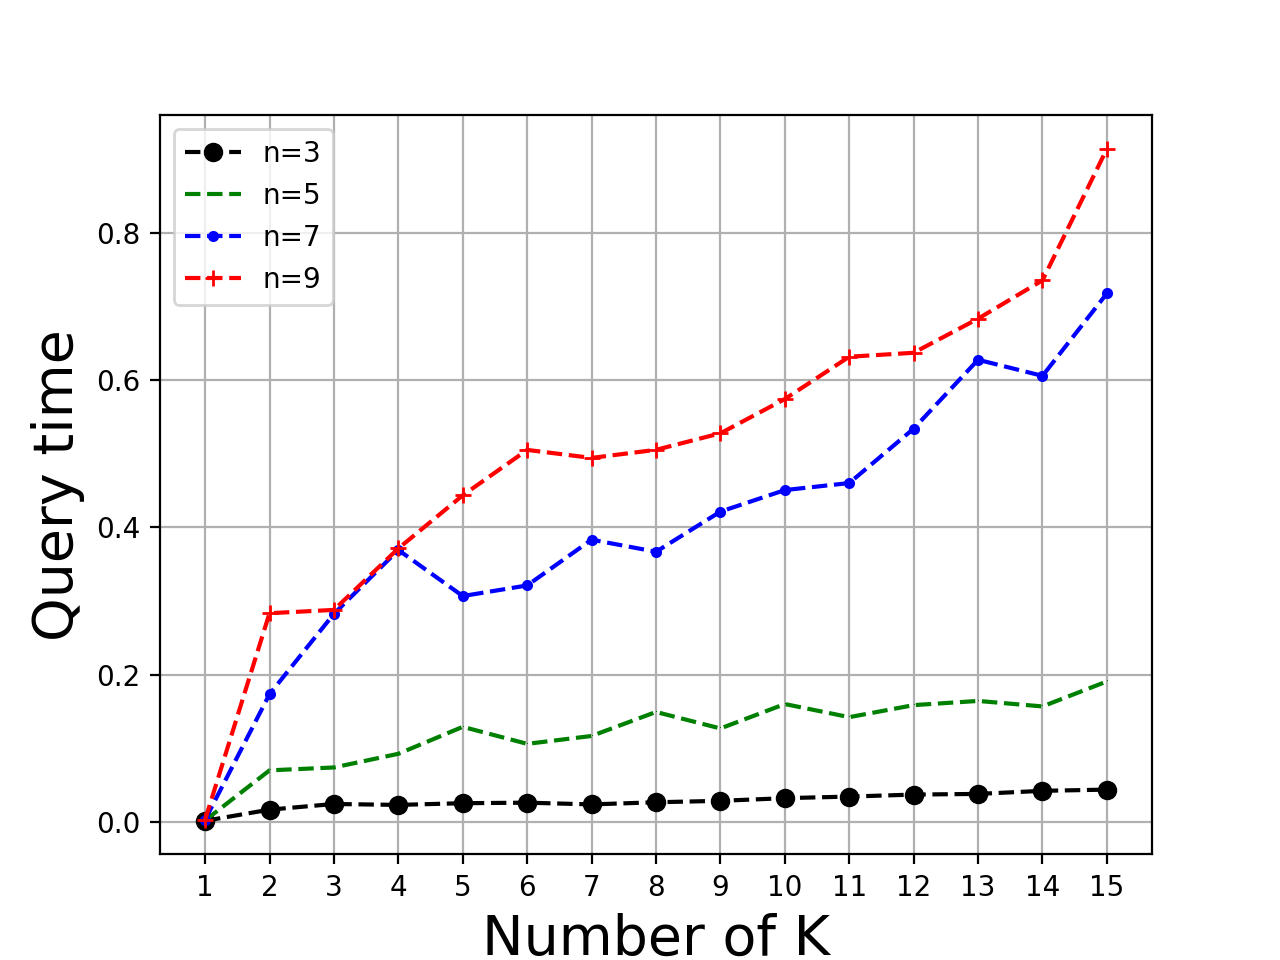
\includegraphics[width=0.45\textwidth]{evaluation/figure1.png}
  \hspace{0.5cm}
  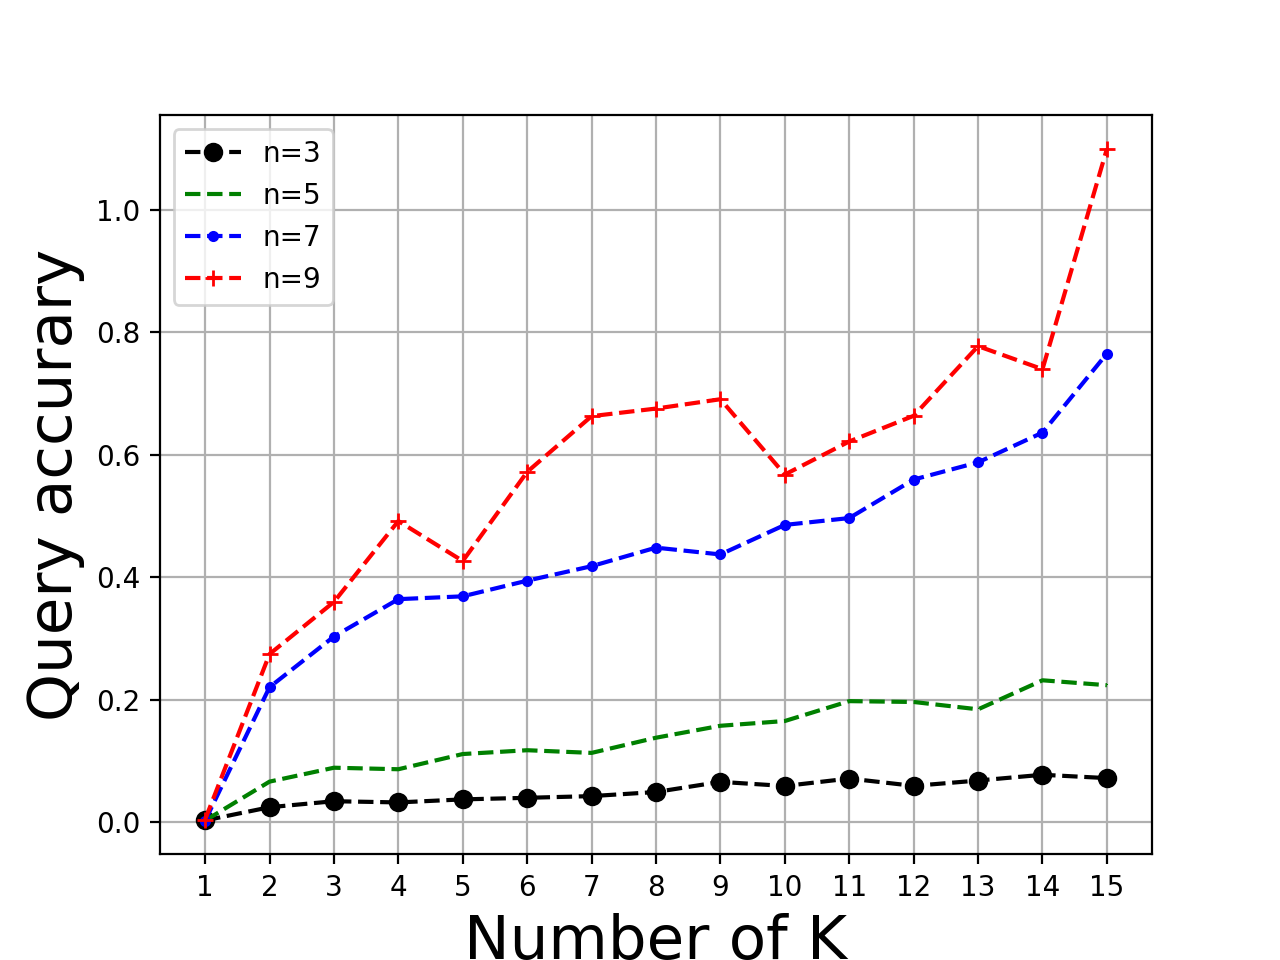
\includegraphics[width=0.45\textwidth]{evaluation/figure2.png}
  \bicaption[fig:number k-time]{相似轨迹查询数目k和查询时间的关系}{相似轨迹查询数目k和查询时间的关系(左图无序查询,有图有序查询)}{Fig}{Query time for the number of k trajectories}
\end{figure}

\begin{figure}[!htp]
  \centering
  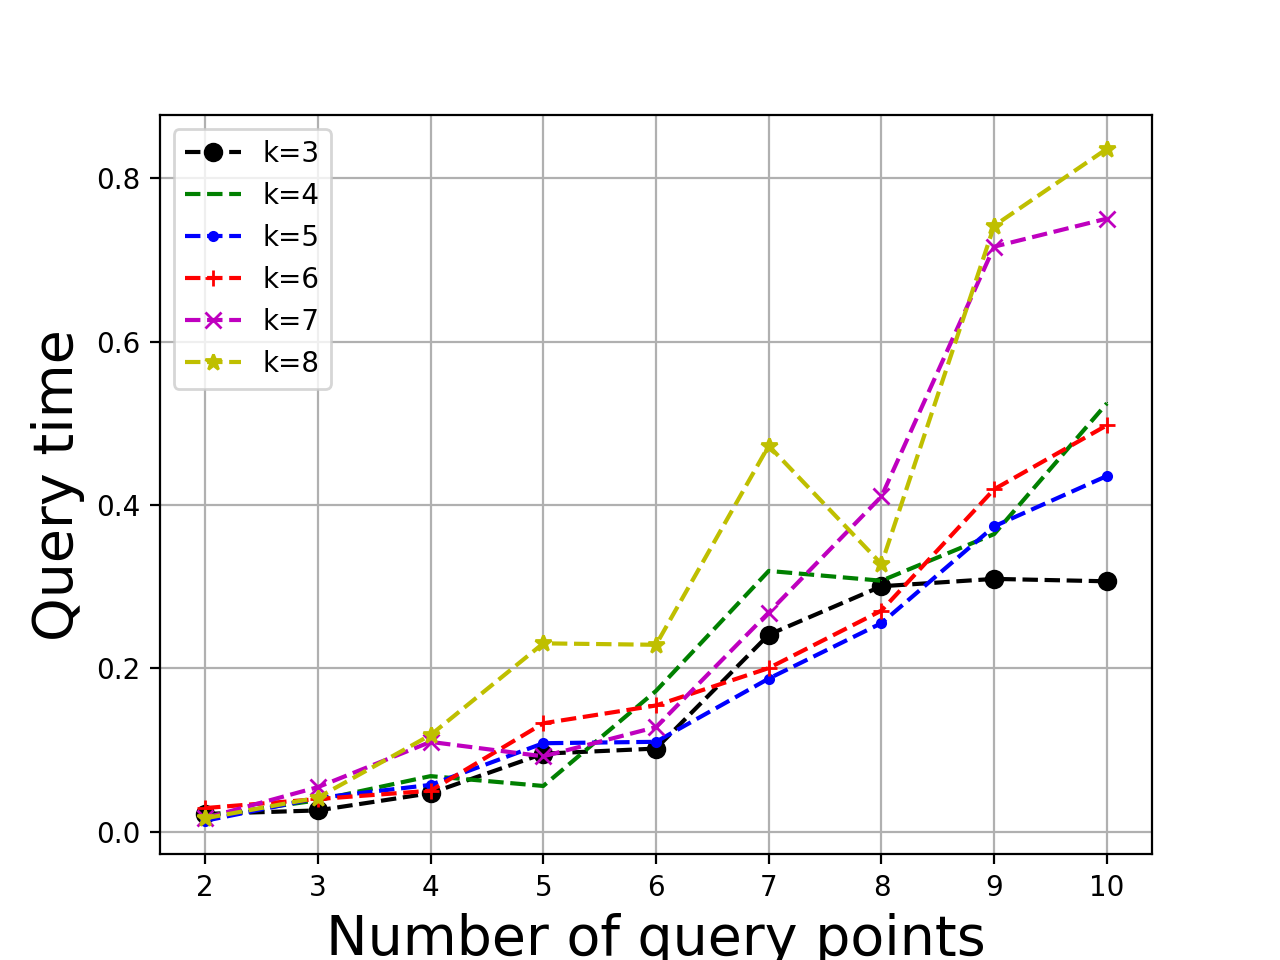
\includegraphics[width=0.45\textwidth]{evaluation/figure3.png}
  \hspace{0.5cm}
  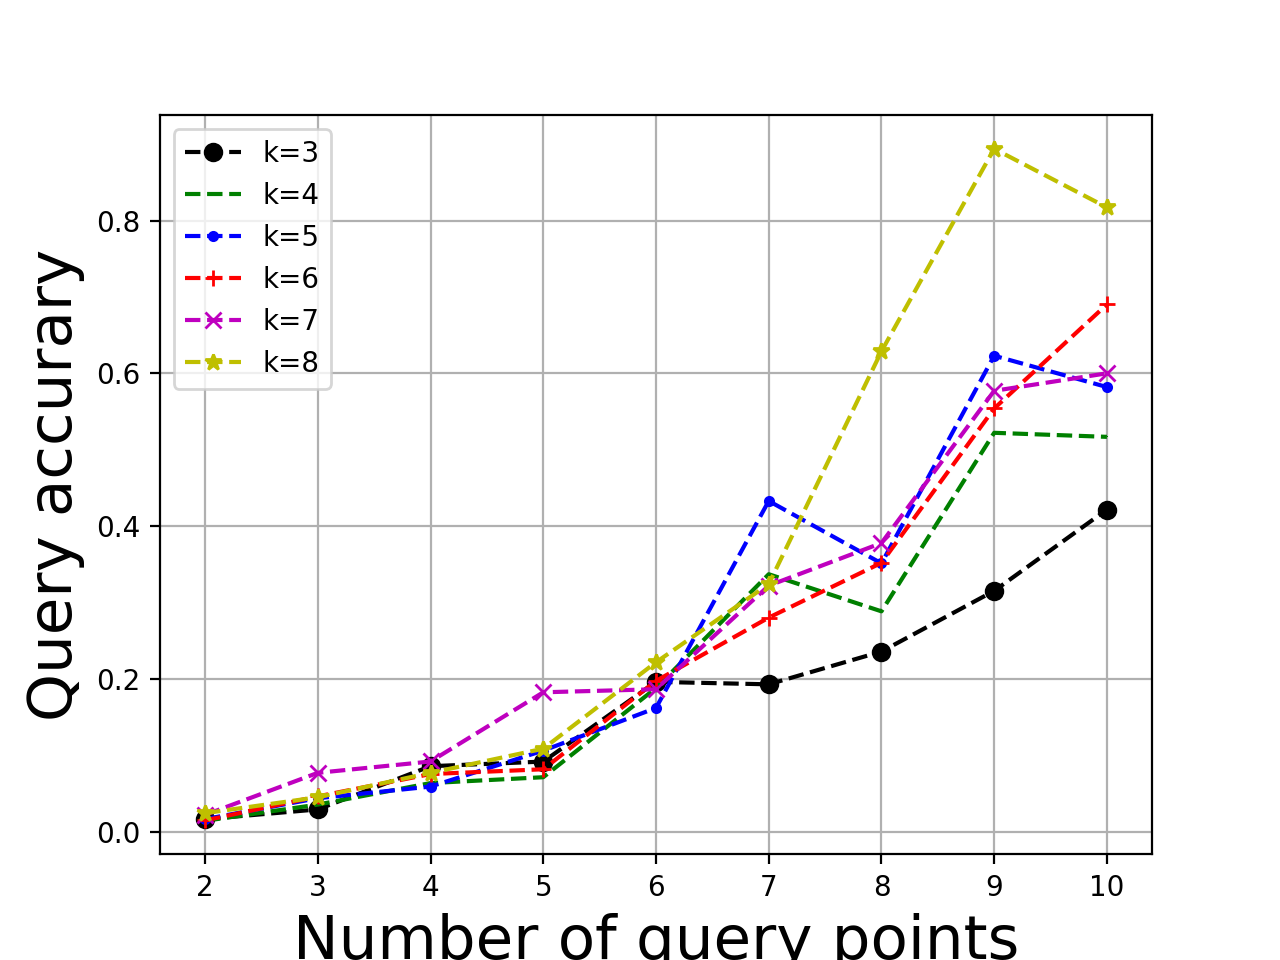
\includegraphics[width=0.45\textwidth]{evaluation/figure4.png}
  \bicaption[fig:number of querypoint-time]{相似轨迹查询点数目和查询时间的关系}{相似轨迹查询点数目和查询时间的关系(左图无序查询,有图有序查询)}{Fig}{Query time for the number of query points}
\end{figure}

\begin{figure}[!htp]
  \centering
  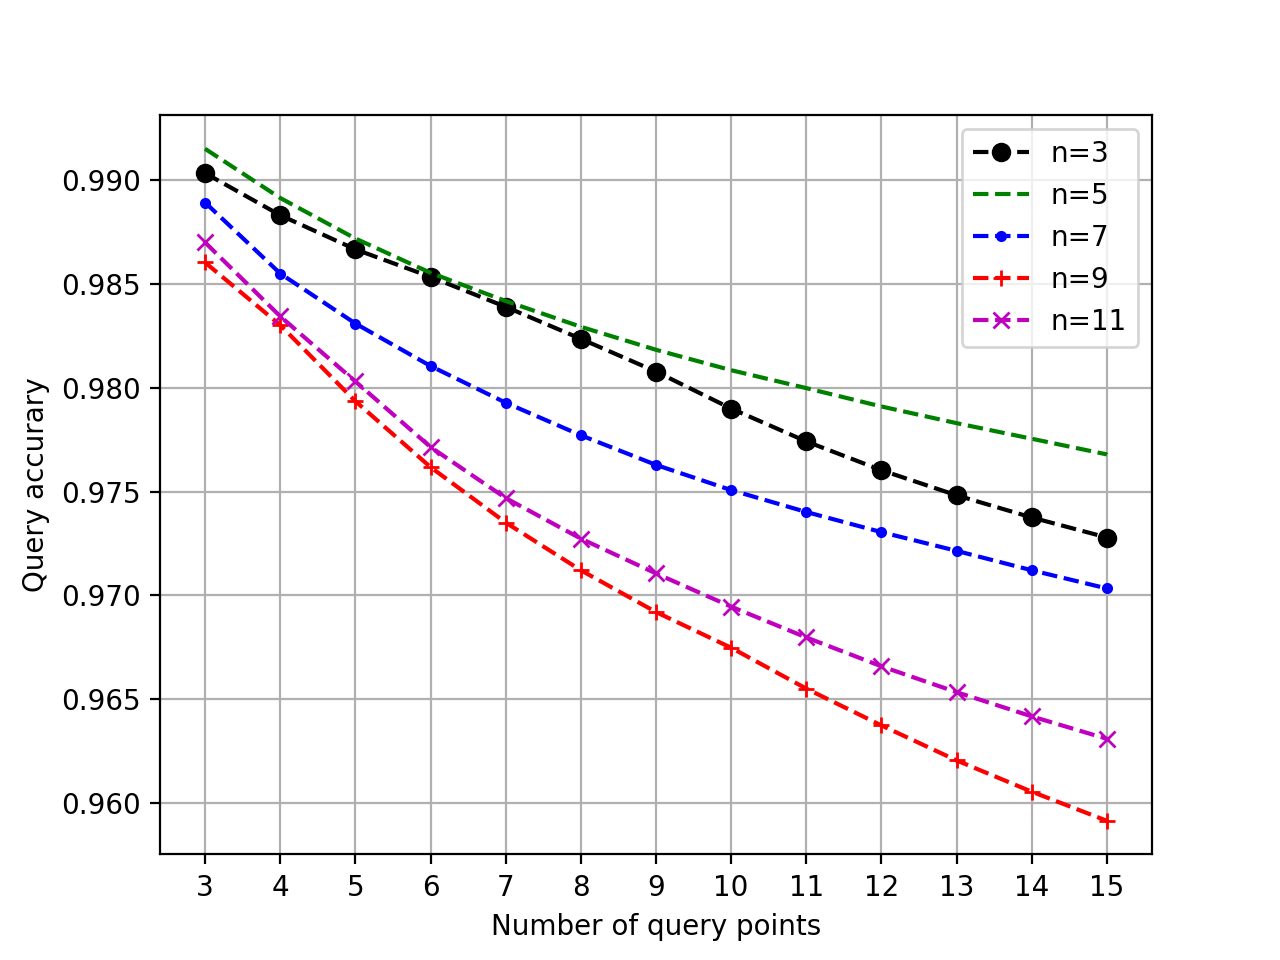
\includegraphics[width=0.45\textwidth]{evaluation/figure5.png}
  \hspace{0.5cm}
  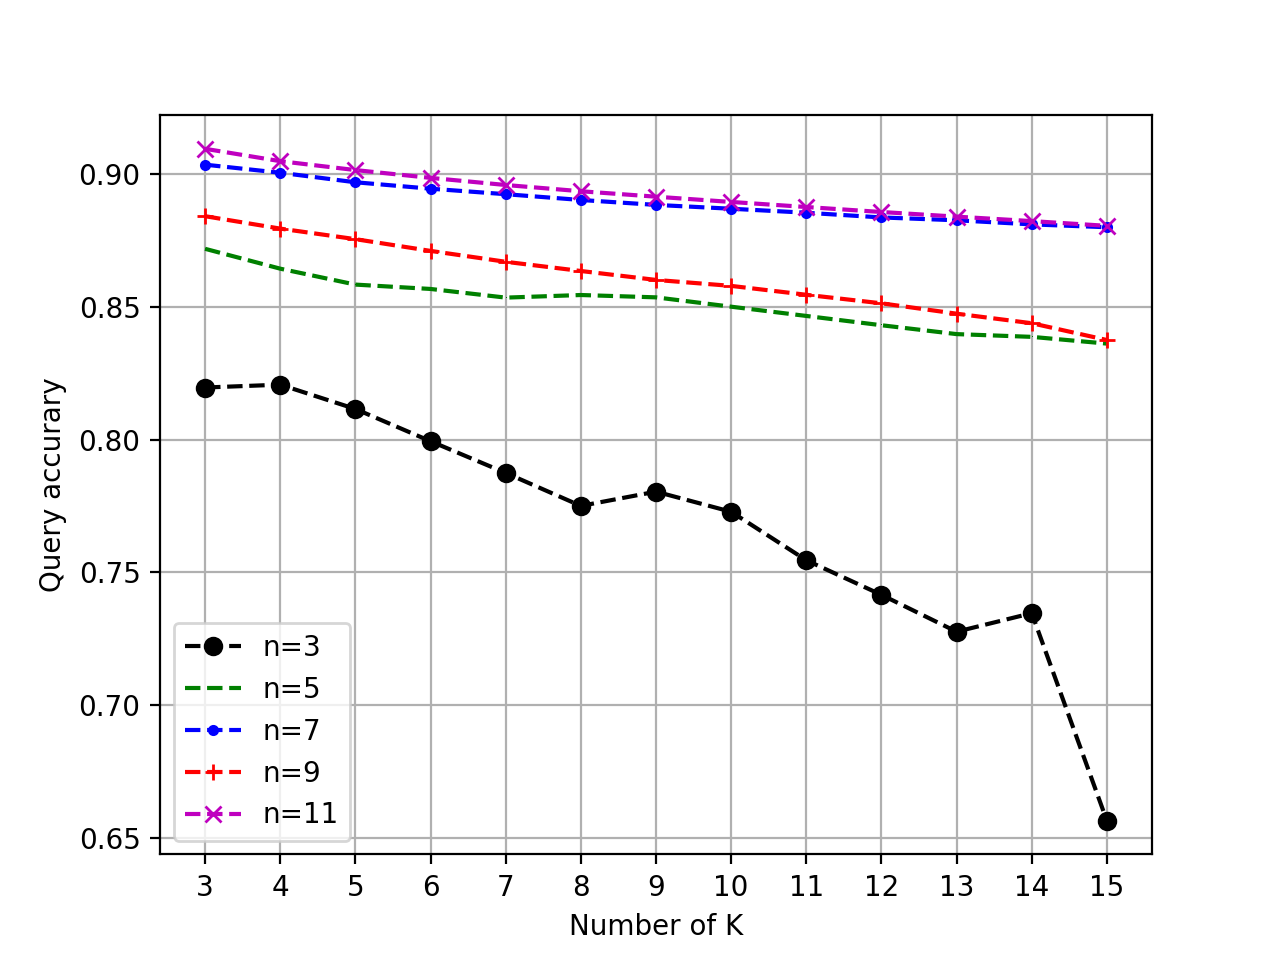
\includegraphics[width=0.45\textwidth]{evaluation/figure6.png}
  \bicaption[fig:number k-accuracy]{相似轨迹查询数目k和查询准确度的关系}{相似轨迹查询数目k和查询准确度的关系(左图无序查询,有图有序查询)}{Fig}{Query accuracy for the number of k trajectories}
\end{figure}

\begin{figure}[!htp]
  \centering
  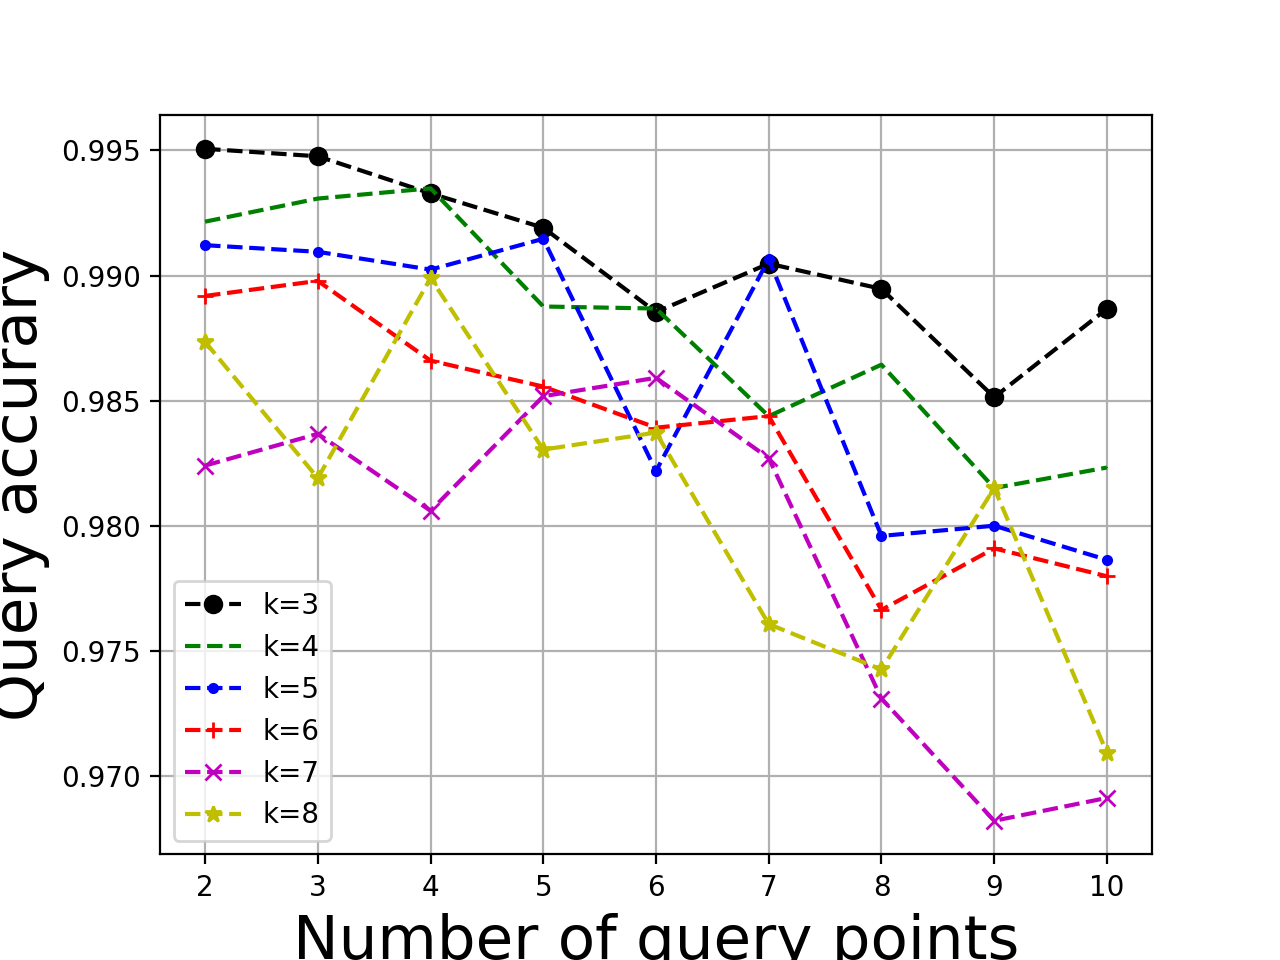
\includegraphics[width=0.45\textwidth]{evaluation/figure7.png}
  \hspace{0.5cm}
  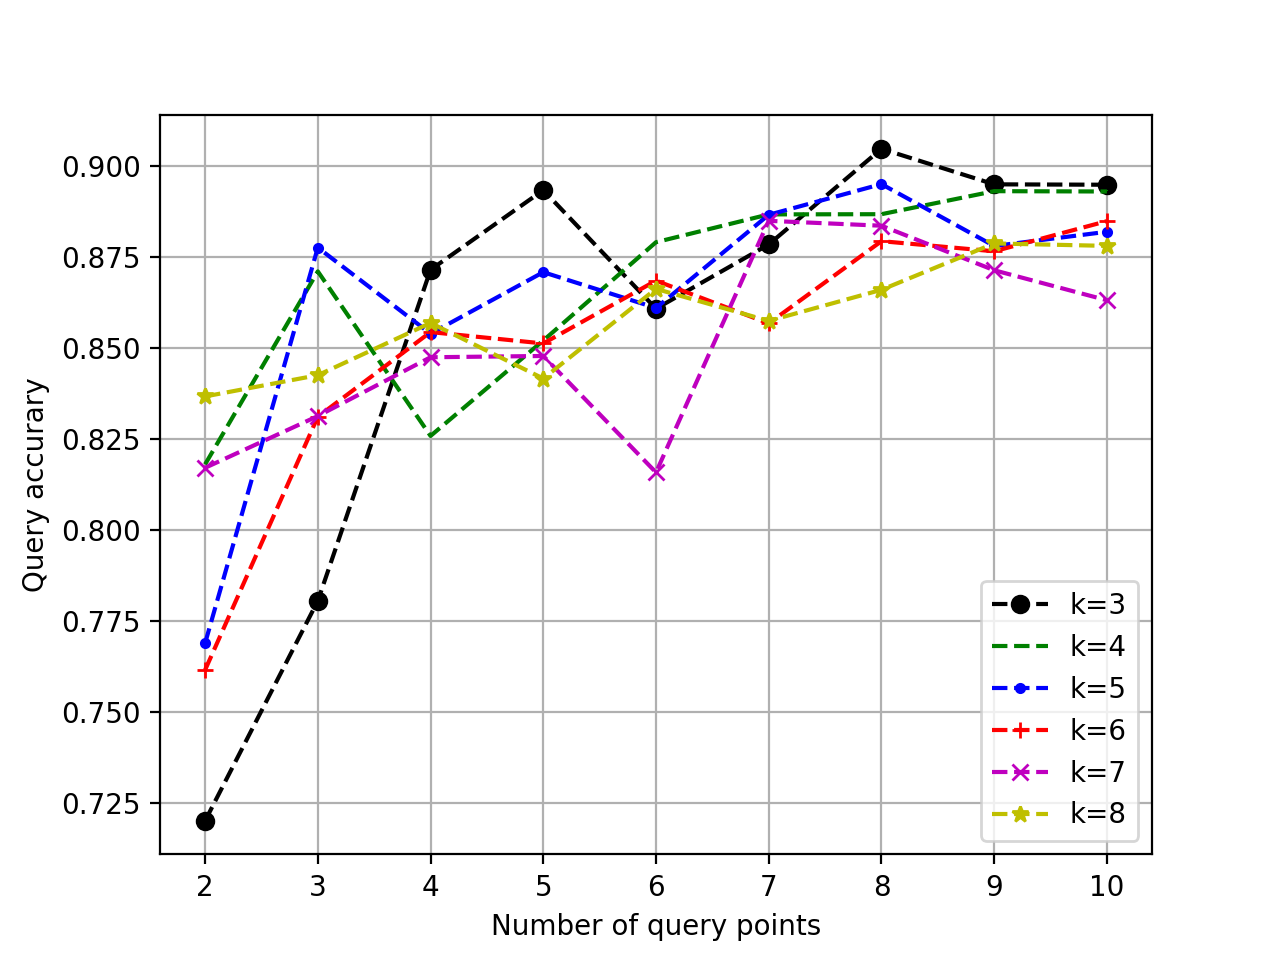
\includegraphics[width=0.45\textwidth]{evaluation/figure8.png}
  \bicaption[fig:number k-accuracy]{相似轨迹查询点数目和查询准确度的关系}{相似轨迹查询点数目和查询准确度的关系(左图无序查询,有图有序查询)}{Fig}{Query accuracy for the number of query points}
\end{figure}

\section{系统测试评价}
\label{sec:system evaluation}
根据上述的测试结果,本文从测试结果所对应的功能和性能两个方面对相似轨迹查询系统做出客观评价。
\begin{itemize}
	\item 从系统功能方面,相似轨迹查询系统完成了以用户为主体对象的用户模块和一部分管理模块功能,初步完成了一个面向用户群里的相似轨迹查询,在必要功能组成上具备完整性。不过功能组成相对简单,在之后基于现阶段的系统设计与实现任务中,应该更多地结合实际应用以丰富完整系统的功能组成。
	\item 从系统性能方面,从测试结果提供的查询时间折线图可以观察得出结论:系统较好地实现了内部的算法部分,单机环境查询结果具有高效性和准确性,能够在大部分实际应用中给予用户良好的查询体验。
	\item 测试过程中也发现了一些不足之处:功能组成相对简单,在之后基于现阶段的系统设计与实现任务中,应该更多地结合实际应用以丰富完整系统的功能组成;性能测试阶段也反应出在测试过程中存在一些误差点,这些误差产生的主要原因主要是由于数据集轨迹较大导致其中中一些噪音点没有预先除去,在之后的测试中应当予以注意。
\end{itemize}

\section{本章小结}
\label{sec:evaluation conclusion}
本章节主要对本文根据相似轨迹查询算法所设计并实现的相似轨迹查询系统进行测试和评价。在测试过程中,参考了目前对软件系统测试的基本方法和理论指导,从功能和性能两个主要方面入手对系统展开测试并得出基本结果。基于这一结果,本文再对系统本文进行评价操作,以符合实际情况。


%# -*- coding: utf-8-unix -*-
%%==================================================
%% chapter05.tex for SJTU Master Thesis
%% based on CASthesis

%%==================================================
\chapter{结论}
\label{chap:conclusion}

\section{待续} %not finished


\appendix	% 使用英文字母对附录编号,重新定义附录中的公式、图图表编号样式
\renewcommand\theequation{\Alph{chapter}--\arabic{equation}}	
\renewcommand\thefigure{\Alph{chapter}--\arabic{figure}}
\renewcommand\thetable{\Alph{chapter}--\arabic{table}}
\renewcommand\thealgorithm{\Alph{chapter}--\arabic{algorithm}}

%% 附录内容,本科学位论文可以用翻译的文献替代。
%\include{tex/app_setup}
%\include{tex/app_eq}
%\include{tex/app_cjk}
%\include{tex/app_log}

\backmatter	% 文后无编号部分 

%% 参考资料
\printbibliography[heading=bibintoc]

%% 致谢、发表论文、申请专利、参与项目、简历
%% 用于盲审的论文需隐去致谢、发表论文、申请专利、参与的项目
\makeatletter

%%
% "研究生学位论文送盲审印刷格式的统一要求"
% http://www.gs.sjtu.edu.cn/inform/3/2015/20151120_123928_738.htm

% 盲审删去删去致谢页
\ifsjtu@review\relax\else
  %# -*- coding: utf-8-unix -*-
\begin{thanks}

  感谢所有测试和使用交大学位论文 \LaTeX 模板的同学!

  感谢那位最先制作出博士学位论文 \LaTeX 模板的交大物理系同学!

  感谢William Wang同学对模板移植做出的巨大贡献!

\end{thanks}
 	  %% 致谢
\fi

\ifsjtu@bachelor
  % 学士学位论文要求在最后有一个英文大摘要,单独编页码
  \pagestyle{biglast}
  %# -*- coding: utf-8-unix -*-
\begin{bigabstract}
Trajectories are the traveling history of moving objects such as a person, a vehicle or an animal. The ever-evolving development in location acquisition and the real-time GPS technology have generated massive spatial trajectory data and can be used for complex analysis across diverse study fields. In this context, a lot of techniques involving mining trajectory data have been fostering a extensive range of applications. The utility of trajectory data depends largely on the efficient and effective trajectory query and search processing in trajectory databases. In fact, trajectory search is aimed to evaluate the spatiotemporal relationships among spatial data objects. Among them, similar trajectory search has long been an attractive and hot topic which helps in various applications in spatial trajectory databases. 

In essence, We design a new type of searching similar trajectory, differing from the conventional ones that finds similar trajectories to a specified one, in which context the query input is only a small number of location points with or without the restraint of order. The target of our searching is substantially to find the k best connected trajectory to the query points, and we consider these result trajectory similar to the query points in the shape geographically. We lay the emphasis more on how well a trajectory connects these query points for the reason that user may focus more on some specific locations when looking for similar trajectory. The basic idea of designing the algorithm is candidate and refinement, which gathers all the potentially similar trajectory as a candidate trajectory set and then preserves k the most similar trajectory as the result to be expected. his novel search type is helpful in many trajectory-related applications such as route planning and trajectory recommendation.

In this paper, we study and fulfil this type of search by the help of k best connected trajectory query. In order to search for the similar trajectory from a large-scale trajectory databases, we are supposed to first define the appropriate similarity function to score how well a trajectory connects the query points. The Eulerian distance function serves well in time of measuring the contribution of each matched points to the similarity. Using the exponential function assists us assign a larger contribute to a closer matched pair of points while lower the dedication of a unmatched or dissimilar ones.

Next, to answer the k best connected query for search similar trajectories. We should first make the full use of the practical observation that the number of query locations tends to be relatively small in general, because users' focuses are impossibly shared to each one of the trajectory points. In this way, we decide to search the k closest trajectories for each query points one by one with the help of existing spatial trajectory indexing and retrieval techniques, and then merge the intermediate query results of each points to generate the final k most similar trajectories. The cost of this method is theoretically considered as the cost of search over the trajectory indexing structure multiplying the number of query points. The latter one can be relatively small upon the above observation. So the cost greatly depends on the indexing structure we adopt. Here, referring some related word, we utilise the commonly used R-tree index while searching the matched points from similar trajectories. After we index the points of all the trajectories from the database by a single R-tree, we can acquire the closest trajectory with regard to a specific query points. This is because if we get the nearest points to a query point, the trajectory that contains this nearest point must be the potential target trajectory to the query points.

Indexing the points in a single R-tree helps us efficiently find the closest trajectory points with regard to a query location. The searching method we adopt is k-NearestNeighbor algorithm. However, this method only cannot handle the searching task because of the incompleteness of single search and process. Therefore, we extend the k-NearestNeighbor to the one with incremental search range, named incremental k-NearestNeighbor, which search the R-tree index continually until the expected similar trajectory are found. The crucial problem in this method is how to prune the unqualified candidate trajectory, refine the possible set of temporary found trajectory and speed up the process of incremental k-NearestNeighbor. In order to handle this key point, we follow to define the lower bound of similarity of the potential trajectories and the upper bound of similarity of unqualified trajectories. By comparing these two similarity, we are able to decide whether the k expected similar trajectories have been contained in the candidate during the searching process, which obviously could tell us when and where to terminate the costly search procedure. 

By using lower bound and upper bound, we have a chance to establish a reasonable pruning strategy for the similar trajectory searching to avoid searching the whole trajectory databases. At this time, one critical question is what search range we should select in the process of searching to promise that the expected k most similar trajectory are found in the candidate set. The dilemma of how to set the search range is that, on one hand, if we set a large value to the search range, it could probably acquire the complete candidate trajectory set at the cost of a huge search space for each query points; on the other hand, the small search range may give rise to the incompleteness of the candidate set that not all the potential trajectories are included in the set and then results in the false dismissal. Given the two bounds mentioned above, we determine to dynamically adjust the search range for the query points respectively, rather than choose the fixed increment for every search loop. With this thought, we initially choose a positive search range for all the query points. However, for each point, if the generated candidate trajectory set cannot satisfy the theorem that determines whether the process is supposed to be stopped, we increase the search region given the search point's weight among the set of query points respectively. Furthermore, taking the decay rate and retrieval ratio as supplemental factors of the query point, we can formulate the proper way to regulate the search range for each point.

The input of search similar trajectory so far is a set of query points. Considering the users' demand, a single trajectory as the input tends to provide a better interactive experience between users and applications. Thus, we combines the current design with trajectory simplification and distributed computing technologies to fulfil the searching of similar trajectory given a specific trajectory in the real world. The input format of a trajectory does not change that the essence of query is the set of query points. But we should choose some points among trajectory points to weigh enough to represent the whole trajectory first. The trajectory simplification based on the locations can handle this concern smoothly by segmenting a trajectory, computing the weight of each point and then choose the number of points important enough to represent a complete trajectory. The simplified result could be relatively large compared to the incremental k-NearestNeighbor algorithm. Now, this paper adopt the distributed computing architecture in the design and implementation. We partition the simplified result to each worker node in the cluster environment and extend the MapReduce programming method. Each worker node can access the trajectory data by Hadoop Distributed File System and then do the search job individually in the map stage as if working in a single machine. The individual results are seen as intermediate and then we merge these results in the reduce stage to select the k most similar trajectory as the final result. The trajectory simplification technique and distributed computing help us extend our method in searching the similar trajectory not only by a set of query points, but also a specific trajectory. Besides, the distributed computing idea can contribute to the multiple requests from many users at the same time, as it can partition the request set and send each of them to one of the worker node.

\end{bigabstract}
\else
  % 盲审论文中,发表学术论文及参与科研情况等仅以第几作者注明即可,不要出现作者或他人姓名
  \ifsjtu@review\relax
    %\include{tex/pubreview}
    %\include{tex/projectsreview}  
  \else
    %\include{tex/pub}	      · %% 发表论文
    %\include{tex/projects}  %% 参与的项目
  \fi
\fi

% \include{tex/patents}	  %% 申请专利
% \include{tex/resume}	  %% 个人简历

\makeatother

\end{document}